\documentclass[10pt,a4paper]{article}

% =============================================================================
% SPRINGER NATURE / JOURNAL OF BIG DATA (FRAMEWORK PAPER SUBMISSION FORMAT)
% =============================================================================
\usepackage[utf8]{inputenc}
\usepackage[T1]{fontenc}
\usepackage{mathptmx}
\usepackage[scaled=0.90]{helvet}
\usepackage{courier}
\usepackage[a4paper,top=24mm,bottom=24mm,left=22mm,right=22mm]{geometry}
\usepackage{amsmath,amsfonts,amssymb}
% Fix mathptmx calligraphic font rendering (\mathcal{M}, \mathcal{B}, \mathcal{R}, \mathcal{E})
\DeclareMathAlphabet{\mathcal}{OMS}{cmsy}{m}{n}
\usepackage{graphicx}
\usepackage{booktabs}
\usepackage{multirow}
\usepackage{array}
\usepackage{xcolor}
\usepackage{fancyhdr}
\usepackage{lastpage}
\usepackage{titlesec}
\usepackage{enumitem}
\usepackage[labelfont={bf,sf,small},textfont={sf,small},labelsep=period]{caption}
\usepackage{xurl}
\usepackage[colorlinks=true,linkcolor=blue!70!black,citecolor=blue!70!black,urlcolor=blue!70!black]{hyperref}

\definecolor{springerblue}{RGB}{0, 102, 153}

% Clean submission running header without placeholder tokens
\pagestyle{fancy}
\fancyhf{}
\fancyhead[L]{\footnotesize\sffamily Noiumkar \quad \textit{Journal of Big Data} --- Research Article Submission}
\fancyhead[R]{\footnotesize\sffamily Page \thepage\ of \pageref*{LastPage}}
\renewcommand{\headrulewidth}{0.4pt}

\titleformat{\section}{\large\sffamily\bfseries\color{springerblue}}{\thesection}{0.6em}{}
\titleformat{\subsection}{\normalsize\sffamily\bfseries}{\thesubsection}{0.6em}{}
\setlength{\parindent}{0pt}
\setlength{\parskip}{0.55em}

\begin{document}

% =============================================================================
% SPRINGEROPEN / JOURNAL OF BIG DATA FRONTMATTER (FRAMEWORK PAPER FRAMING)
% =============================================================================
{\footnotesize\sffamily\color{springerblue}\textbf{RESEARCH ARTICLE} \hfill \textbf{Journal of Big Data (SpringerOpen)}}\\[0.8em]

{\LARGE\sffamily\bfseries AST-Route: An AST-Aware Multi-Objective Query Routing and Cost-Prediction Framework Across Serverless Cloud, Vectorized CPU (C++/Rust), and GPU-Accelerated OLAP Engines}\\[0.9em]

{\normalsize\sffamily\textbf{Preecha Noiumkar}\textsuperscript{1*}}\\[0.4em]
{\footnotesize\sffamily
\textsuperscript{1}Department of Information Technology, Faculty of Informatics, Mahasarakham University, Kham Riang, Kantharawichai, Maha Sarakham 44150, Thailand.\\
\textsuperscript{*}Correspondence: Preecha Noiumkar (\href{mailto:preecha.n@msu.ac.th}{preecha.n@msu.ac.th})
}\\[0.8em]

\noindent\rule{\textwidth}{0.8pt}
\begin{quote}
\small\sffamily
\textbf{\color{springerblue}Abstract}\\[0.3em]
\textbf{Background:} Modern analytical data infrastructures span heterogeneous execution paradigms, including serverless cloud data warehouses, in-process C++ and Rust Apache Arrow vectorized CPU engines, and SIMT GPU-accelerated relational engines. However, no single engine dominates across all query topologies and data scales: low-complexity scans suffer from PCIe host-to-device transfer penalties on GPUs and scheduling overheads on serverless clouds, complex window sorting and lateral array unnesting overwhelm single-node CPU pipelines, and datasets exceeding device VRAM or host DRAM ($\text{SF}=10, 30, \text{and } 100\text{ GB}$) trigger out-of-core disk spilling and chunked PCIe streaming bottlenecks. Existing systems lack a unified, pre-execution routing framework capable of predicting multi-engine execution latency, hardware energy footprint, memory spilling, and cloud financial cost directly from static query structure and predicate selectivity.\\[0.25em]
\textbf{Methodology:} We propose \textbf{AST-Route}, a four-layer AST-Aware Multi-Objective Query Routing and Cost-Prediction Framework. Layer 1 parses input SQL queries into a 9-dimensional feature vector ($\mathbf{x}_q \in \mathbb{R}^9$) combining static Abstract Syntax Tree (AST) structural operators---tree depth, total AST nodes, multi-way join fan-out, nested CTEs/subqueries, window frames, conditional branches, array unnesting (\texttt{UNNEST}), and a construct-validated Composite Structural Complexity Index (CSCI, mean $29.66$, 10,000-trial Monte Carlo rank stability $\bar{\rho}=0.9880$ at $\pm 20\%$ weight perturbation and $\rho=0.9812$ against equal weights)---with lightweight zone-map predicate selectivity ($\sigma(q)$). Layer 2 formulates cross-paradigm analytical models governing the PCIe bottleneck crossover ($\Phi_{\text{PCIe}}$), effective scan throughput ($\Theta_{\text{eff}}$), slot-to-wall concurrency proxy ($\mathcal{M}_{\text{slot}}$), FinOps savings ($\Delta C_{\text{1M}}$), and Green OLAP energy efficiency ($\eta_{\text{watt}}$). Layer 3 employs a Multi-Output Gradient Boosting Regressor ($\mathcal{R}_{\text{GBR-9D}}$) to simultaneously predict execution latency, energy consumption, and memory footprint across candidate engines, while Layer 4 dispatches queries via a configurable latency--energy Pareto objective ($\alpha \in [0,1]$). Following the official TPC-H discrete scale factor specification ($\text{SF} \in \{1, 10, 30, 100\text{ GB}\}$), we validate the framework under a strict zero-estimation, 100\% real execution and GPU/CPU fairness protocol (64-bit IEEE 754 \texttt{FP64} precision symmetry and unrestricted multi-core SIMD threading) across: (i) a 75-query TPC-H-derived AST-stratified factorial workload (25 canonical seeds $\times$ 3 selectivity horizons, L1--L5), (ii) the 22 official standard TPC-H benchmark queries (Q1--Q22), (iii) four standard scale factors spanning $\text{SF}=1\text{ GB}$ ($6.0\text{M}$ \texttt{lineitem} rows / $8.7\text{M}$ total rows), $\text{SF}=10\text{ GB}$ ($60.0\text{M}$ / $86.6\text{M}$ rows), $\text{SF}=30\text{ GB}$ ($180.0\text{M}$ / $259.8\text{M}$ rows), and $\text{SF}=100\text{ GB}$ ($600.1\text{M}$ / $866.1\text{M}$ rows), and (iv) three cross-platform hardware profiles (2-core/4GB container, 4-core/8GB node, and 8-core/16GB workstation with an NVIDIA GeForce RTX 2050 $4.0\text{ GB}$ VRAM GPU) across six engines: Google BigQuery, DuckDB, Polars, Apache DataFusion, SQLite 3, and a PyTorch CUDA Tensor Engine.\\[0.25em]
\textbf{Results:} At $\text{SF}=1\text{ GB}$, ground-truth telemetry confirms highly significant cross-engine stratification ($\chi^2_F(5) = 321.50, p = 2.382 \times 10^{-67}$, Kendall's $W = 0.8573$, $100.0\%$ \texttt{FP64} equivalence $\text{EX}=1$). Vectorized CPU engines---Polars ($82.47\text{ ms}$, 95\% CI: $[67.93, 98.65]\text{ ms}$), DataFusion ($96.30\text{ ms}$), and DuckDB ($183.74\text{ ms}$)---outperform the row-store baseline ($8417.33\text{ ms}$; Cliff's $\delta = +1.000, p = 5.28 \times 10^{-14}$) by $45.8\times\text{--}102.1\times$ while reducing per-query energy from $126.26\text{ J}$ to $3.17\text{--}6.40\text{ J}$. BigQuery clustering reduces server latency from $1412.6\text{ ms}$ to $745.39\text{ ms}$ (Cliff's $\delta = +0.471$) and prunes V1 I/O by $78.4\%$ ($\$1.47\text{--}\$147.00\text{ USD/1M}$ savings across $\text{SF}=1\text{--}100\text{ GB}$), while RTX 2050 GPU execution ($1.30\text{ GB}$ VRAM) achieves $56.96\text{ ms}$ cold ($0.65\text{ J}$) and $22.26\text{ ms}$ warm latency ($0.25\text{ J}$, $1942.8\text{ MB/J}$). Evaluated via 25-seed LOSO-CV, \textbf{AST-Route} ($\mathcal{R}_{\text{GBR-9D}}$) predicts multi-engine costs with low multiplicative Q-Error (Median P50 Q-Error: $1.007\text{--}1.172$; $R^2 = 0.815\text{--}0.875$) in $497.2\text{ }\mu\text{s}$ ($4.145\text{ ms}$ total parsing and routing overhead), achieving $57.33\%$ Top-1 accuracy ($65.33\%$ near-optimal hits), $54.92\text{ ms}$ mean latency ($0.00\%$ median regret, $34.98\%$ mean regret), and $1.381\text{ J}$ energy---outperforming Always DuckDB ($3.35\times, p=1.83\times 10^{-6}$), Always Polars ($1.50\times, p=1.47\times 10^{-6}$), Always GPU, Always BigQuery, and Rule-Based Routing ($p = 0.0187$, $2.83\times$ faster in L5). Furthermore, \textbf{AST-Route} achieves $73.33\%$ Top-1 accuracy ($47.01\text{ ms}$) on 5 locked unseen holdout seeds, $40.91\%\text{--}72.73\%$ Top-1 accuracy ($15.84\text{--}27.33\text{ ms}$ mean latency) on the 22 official TPC-H queries (Q1--Q22), and $4.63\times\text{--}7.63\times$ speedups across $\text{SF}=1, 10, 30, \text{and } 100\text{ GB}$ ($9.18\times$ cross-platform speedup on 8-core+GPU workstations vs. CPU baselines), capturing the progressive memory-wall transition as host RAM caps at $9.00\text{ GB}$ ($0 \rightarrow 125 \rightarrow 864 \rightarrow 3302\text{ MB}$ disk spill) and GPU PCIe streaming scales across $1\times, 4\times, 12\times, \text{and } 40\times$ chunks ($1.30 \rightarrow 3.45 \rightarrow 3.68 \rightarrow 3.85\text{ GB}$ VRAM).\\[0.25em]
\textbf{Conclusion:} \textbf{AST-Route} provides a lightweight, leak-free, and scale-aware query routing framework that generalizes across unseen SQL templates, standard TPC-H Q1--Q22 workloads, and $\text{SF}=1, 10, 30, \text{and } 100\text{ GB}$ data scales. All code, workloads, and SHA-256 telemetry logs are publicly available at \url{https://github.com/preecha-msu/bigquery-olap-benchmark}.\\[0.45em]
\textbf{\color{springerblue}Keywords:} Abstract syntax tree (AST), Apache Arrow, Apache DataFusion, Automated query routing framework, Columnar storage, CUDA GPU acceleration, DuckDB, Energy efficiency, Google BigQuery, Polars, TPC-H benchmark.
\end{quote}
\noindent\rule{\textwidth}{0.8pt}

% =============================================================================
% 1. INTRODUCTION
% =============================================================================
\section{Introduction}
Modern enterprise analytics increasingly operate over heterogeneous, polyglot data infrastructures spanning four distinct computing paradigms: elastic serverless cloud data warehouses such as Google BigQuery \cite{melnik2010dremel,melnik2020dremel,lounissi2025funda}, in-process C++ vectorized analytical database systems such as DuckDB \cite{raasveldt2019duckdb,kuiper2024duckdb_ooc}, Rust-based Apache Arrow streaming query engines such as Polars and Apache DataFusion \cite{lamb2024datafusion}, and SIMT GPU-accelerated relational engines \cite{chrysogelos2019hetexchange,shanbhag2020crystal}, alongside distributed multi-node systems like ClickHouse \cite{schulze2024clickhouse} and Trino \cite{sethi2019presto}. While cloud-native disaggregated storage-compute architectures provide massive horizontal slot concurrency for petabyte-scale workloads \cite{shojaee2024serverless,abdalla2022bigdata}, they introduce non-trivial stateless scheduling and distributed shuffle overheads on moderate-scale datasets \cite{begoli2018calcite,garcia2008database,lounissi2025funda}. Concurrently, modern local hardware presents an intricate architectural trade-off between CPU SIMD vectorization over Apache Arrow memory buffers and discrete GPU offloading across the PCIe interconnect \cite{milicevic2024dlquery,root2019mapd,kim2022blazingsql}.

Because each execution paradigm exhibits fundamentally different algorithmic strengths and memory-hierarchy bottlenecks across the discrete scale factors defined by the Transaction Processing Performance Council ($\text{SF} \in \{1, 10, 30, 100\text{ GB}\}$ in the TPC-H specification \cite{tpc2022tpch,boncz2014tpch,dreseler2020quantifying}), committing an entire analytical workload to any single static engine results in severe performance regret, excessive energy consumption, out-of-core spilling penalties, or unnecessary cloud FinOps expenditure. Designing an automated, pre-execution query routing framework capable of dynamically dispatching SQL queries to their optimal execution backend requires overcoming three critical research gaps in the existing literature \cite{ahmed2020hibench,oneil2009ssb,leis2015job}:
\begin{itemize}[leftmargin=1.5em,itemsep=2pt]
    \item \textbf{Research Gap 1 (Lack of Pre-Execution Cross-Paradigm Query Routing Frameworks):} Existing learned query optimizers such as Neo \cite{marcus2019neo} and Bao \cite{marcus2021bao} steer physical operator plans \emph{within} a single database engine, while cloud workload routers \cite{tan2023stage} assign jobs across homogeneous cloud clusters. There is currently no unified, lightweight routing framework that extracts static Abstract Syntax Tree (AST) features and zone-map selectivity prior to execution to route queries across heterogeneous C++ DBMS, Rust Arrow, CUDA GPU, and serverless cloud engines.
    \item \textbf{Research Gap 2 (Unmodeled PCIe Crossover Thresholds, Memory Walls, and Green OLAP Energy Costs):} Prior GPU database studies \cite{shanbhag2020crystal,root2019mapd,kim2022blazingsql} predominantly report warm in-VRAM kernel speedups at fixed small scale factors ($\text{SF}=1\text{ GB}$) while omitting cold-start PCIe Host-to-Device (H2D) transfer overheads, chunked PCIe streaming when datasets exceed device VRAM ($\text{SF}=10, 30, \text{and } 100\text{ GB}$), out-of-core host RAM disk spilling \cite{kuiper2024duckdb_ooc}, and hardware energy efficiency ($\text{Joules}$ and $\text{MB/J}$).
    \item \textbf{Research Gap 3 (Confounded Complexity, Data Leakage, and Lack of Cross-Workload Transfer):} Traditional OLAP evaluations \cite{ahmed2020hibench,abdalla2022bigdata} rely on unstratified query sets where structural operator depth, storage layout (row-store vs. Parquet vs. Arrow), and predicate selectivity are confounded, and where random train-test splits across variations of the same query template induce severe data leakage without testing generalization to unseen seeds or standard TPC-H Q1--Q22 choke-point workloads \cite{boncz2014tpch,dreseler2020quantifying}.
\end{itemize}

To address these gaps under a strict \emph{zero-estimation, 100\% real execution} protocol, we propose \textbf{AST-Route}, an AST-Aware Multi-Objective Query Routing and Cost-Prediction Framework. This study makes five primary contributions:
\begin{enumerate}[leftmargin=1.5em,itemsep=2pt]
    \item \textbf{The AST-Route Four-Layer Framework and Construct-Validated CSCI:} We design a four-layer routing architecture (Fig.~\ref{fig:proposed_ast_framework}) that parses arbitrary SQL queries into a 9-dimensional structural and selectivity vector ($\mathbf{x}_q \in \mathbb{R}^9$). We formulate and empirically validate the Composite Structural Complexity Index ($\text{CSCI}$) across a 75-query TPC-H-derived factorial workload (25 canonical seeds $\times$ 3 selectivity horizons, L1--L5) and the 22 official TPC-H queries (Q1--Q22) \cite{tpc2022tpch}, demonstrating significant rank correlation with GPU kernel speedup (Spearman's $\rho=0.4935, p=6.84\times 10^{-6}$) and high invariance under 10,000-trial Monte Carlo weight perturbation ($\bar{\rho}=0.9880$ at $\pm 20\%$ and $\bar{\rho}=0.9555$ at $\pm 50\%$).
    \item \textbf{Unified Analytical Crossover, FinOps, and Green Energy Formulation:} Within the framework's cost layer, we establish formal mathematical models for the GPU PCIe bottleneck fraction ($\Phi_{\text{PCIe}}$) and break-even condition, effective scan throughput ($\Theta_{\text{eff}}$), slot-to-wall concurrency proxy ($\mathcal{M}_{\text{slot}}$), FinOps cost savings ($\Delta C_{\text{1M}}$), and Green OLAP performance per watt ($\eta_{\text{watt}}$).
    \item \textbf{Six-Engine Ground-Truth Telemetry Testbed with GPU/CPU Fairness and Seed-Clustered 95\% CIs:} We construct a full-scale multi-paradigm testbed spanning six canonical software engines---SQLite 3, Google BigQuery, DuckDB, Polars, Apache DataFusion, and a hardware-timed CUDA Tensor Engine on an NVIDIA GeForce RTX 2050 GPU---enforcing strict \texttt{FP64} numerical parity ($\epsilon < 10^{-9}$), unrestricted multi-core CPU SIMD threading, and 10,000-iteration bootstrap 95\% CIs with Cliff's delta ($\delta$) effect sizes.
    \item \textbf{Multi-Output Q-Error Cost Prediction, Leak-Free LOSO-CV, and Unseen Seed Generalization:} We validate \textbf{AST-Route} ($\mathcal{R}_{\text{GBR-9D}}$) via 25-seed LOSO-CV and a strict unseen holdout split (training on 20 development seeds \texttt{S1}--\texttt{S4} and testing on 5 locked unseen seeds \texttt{L1\_S5}--\texttt{L5\_S5}), achieving median Q-Errors of $1.007\text{--}1.172$, $54.92\text{ ms}$ LOSO-CV latency ($0.00\%$ median regret), and $73.33\%$ Top-1 accuracy ($47.01\text{ ms}$ mean latency) on completely unseen query seeds.
    \item \textbf{Four-Scale Big Data Evaluation ($\text{SF}=1, 10, 30, \text{and } 100\text{ GB}$), Official TPC-H Q1--Q22, and Cross-Platform Validation:} Adhering to the official TPC-H benchmark scale tiers \cite{tpc2022tpch,dreseler2020quantifying}, we scale execution across four standard scale factors from $6.0\text{M}$ to $600.1\text{M}$ \texttt{lineitem} rows ($8.7\text{M}$ to $866.1\text{M}$ total rows), profiling out-of-core host RAM spilling ($0 \rightarrow 125 \rightarrow 864 \rightarrow 3302\text{ MB}$), chunked GPU PCIe streaming ($1\times \rightarrow 4\times \rightarrow 12\times \rightarrow 40\times$ chunks across the $4.0\text{ GB}$ VRAM wall), cross-platform hardware scaling (2, 4, and 8 cores across all four scale factors), and official TPC-H Q1--Q22 routing ($15.84\text{--}27.33\text{ ms}$ mean latency).
\end{enumerate}

% =============================================================================
% 2. RELATED WORK
% =============================================================================
\section{Related Work and Architectural Representativeness}
\subsection{Cloud MPP Warehouses, Distributed Query Engines, and Vectorized CPU Systems}
Disaggregated cloud data warehouses pioneered by Google Dremel/BigQuery \cite{melnik2010dremel,melnik2020dremel} and distributed MPP query engines such as Presto/Trino \cite{sethi2019presto}, ClickHouse \cite{schulze2024clickhouse}, and Apache Spark \cite{ahmed2020hibench} decouple compute workers from durable storage. Recent studies in serverless data pipelines \cite{shojaee2024serverless} and in-situ serverless query processing such as FunDa \cite{lounissi2025funda} highlight the fundamental tension between cold-start scheduling overhead and horizontal slot elasticity. Specifically, while Trino \cite{sethi2019presto} excels at federated cross-source query execution over distributed object stores and ClickHouse \cite{schulze2024clickhouse} achieves high throughput via shared-nothing merge-tree storage and SIMD vectorization across cluster nodes, both introduce network serialization and coordinator scheduling overheads when deployed on single-node or moderate-scale datasets. Conversely, embeddable C++ vectorized engines such as DuckDB \cite{raasveldt2019duckdb,kuiper2024duckdb_ooc} process columnar Row Groups in-process using morsel-driven parallelism and out-of-core external memory management, whereas next-generation Rust engines (Polars and Apache DataFusion \cite{lamb2024datafusion}) execute zero-copy SIMD and streaming pipelines directly over standardized Apache Arrow memory buffers.

\subsection{GPU-Accelerated Databases, Learned Query Optimizers, and OLAP Benchmarks}
In the domain of GPU-accelerated relational analytics, systems such as HeavyDB (formerly OmniSci/MapD) \cite{root2019mapd}, BlazingSQL over RAPIDS cuDF \cite{kim2022blazingsql}, Crystal \cite{shanbhag2020crystal}, and HetExchange \cite{chrysogelos2019hetexchange} leverage massive SIMT parallelism and high-bandwidth device memory (VRAM) to accelerate relational joins and group-by aggregations. However, as demonstrated by Chrysogelos et al. \cite{chrysogelos2019hetexchange} and Shanbhag et al. \cite{shanbhag2020crystal}, discrete GPU execution is fundamentally constrained by the PCIe interconnect when data resides in host DRAM or exceeds device VRAM capacity, necessitating rigorous separation of PCIe transfer latency from kernel compute time. Concurrently, recent surveys on deep learning in query execution \cite{milicevic2024dlquery} and learned optimizers---including Neo \cite{marcus2019neo}, Bao \cite{marcus2021bao}, Zero-Shot Cost Models \cite{hilprecht2022zeroshot}, and stage-level cloud routers \cite{tan2023stage}---demonstrate that structural query features can guide physical execution decisions. In parallel, the TPC-H decision support benchmark specification \cite{tpc2022tpch} establishes discrete scale factors ($\text{SF}=1, 10, 30, 100\text{ GB}$) and 22 canonical queries (Q1--Q22) whose internal execution choke points have been formalized by Boncz et al. \cite{boncz2014tpch} and Dreseler et al. \cite{dreseler2020quantifying}. Complementing classical OLAP benchmarks such as the Star Schema Benchmark (SSB) \cite{oneil2009ssb} and the Join Order Benchmark (JOB) \cite{leis2015job}, modern text-to-SQL benchmarks such as BIRD \cite{li2023bird} and Spider 2.0 \cite{lei2025spider2} incorporate the Valid Efficiency Score (VES), while AST transpilers such as \texttt{SQLGlot} \cite{mao2024sqlglot} and Apache Calcite \cite{begoli2018calcite} enable deterministic structural analysis.

\subsection{Rationale for Target Execution Engines in the AST-Route Framework}
Rather than exhaustively evaluating every commercial DBMS, \textbf{AST-Route} targets six software engines that serve as canonical, non-redundant representatives of the four foundational execution paradigms in modern data engineering:
\begin{enumerate}[leftmargin=1.5em,itemsep=2pt]
    \item \textbf{SQLite 3 (Canonical Tuple-at-a-Time B-Tree Row-Store Baseline):} Represents traditional ANSI C row-oriented storage using a Volcano-style iterator model, establishing the exact performance and energy baseline of B-tree page traversal without columnar compression or SIMD vectorization.
    \item \textbf{Google BigQuery (Canonical Serverless Disaggregated Cloud OLAP):} Represents petabyte-scale cloud-native execution (Dremel/Capacitor columnar storage with dynamic slot allocation) \cite{melnik2020dremel}, isolating distributed cloud orchestration overhead and storage clustering FinOps economics without local hardware bottlenecks.
    \item \textbf{DuckDB (Canonical C++ Morsel-Driven Columnar DBMS):} Represents state-of-the-art in-process C++ analytical database design \cite{raasveldt2019duckdb,kuiper2024duckdb_ooc} with tightly integrated storage block management, parallel segment-tree window framing, and out-of-core external disk spilling.
    \item \textbf{Polars \& Apache DataFusion (Canonical Rust Apache Arrow Engines):} Represent the emerging Rust Arrow ecosystem via two distinct optimizer philosophies: \emph{Polars} exemplifies a dataframe-native lazy streaming engine over Arrow arrays, whereas \emph{Apache DataFusion} \cite{lamb2024datafusion} exemplifies a modular SQL physical query planner (used as the core execution engine in modern distributed systems such as InfluxDB 3.0 and Ballista).
    \item \textbf{PyTorch CUDA Relational Tensor Engine (Canonical SIMT GPU Execution):} Represents hardware-timed GPU relational tensor processing over contiguous device buffers (analogous to cuDF/BlazingSQL \cite{kim2022blazingsql} and Crystal \cite{shanbhag2020crystal}), enabling exact hardware-counter decomposition of PCIe H2D transfers, chunked out-of-VRAM streaming, and in-VRAM SIMT kernel execution on consumer/edge GPU hardware (NVIDIA RTX 2050).
\end{enumerate}

\begin{figure}[t!]
\centering
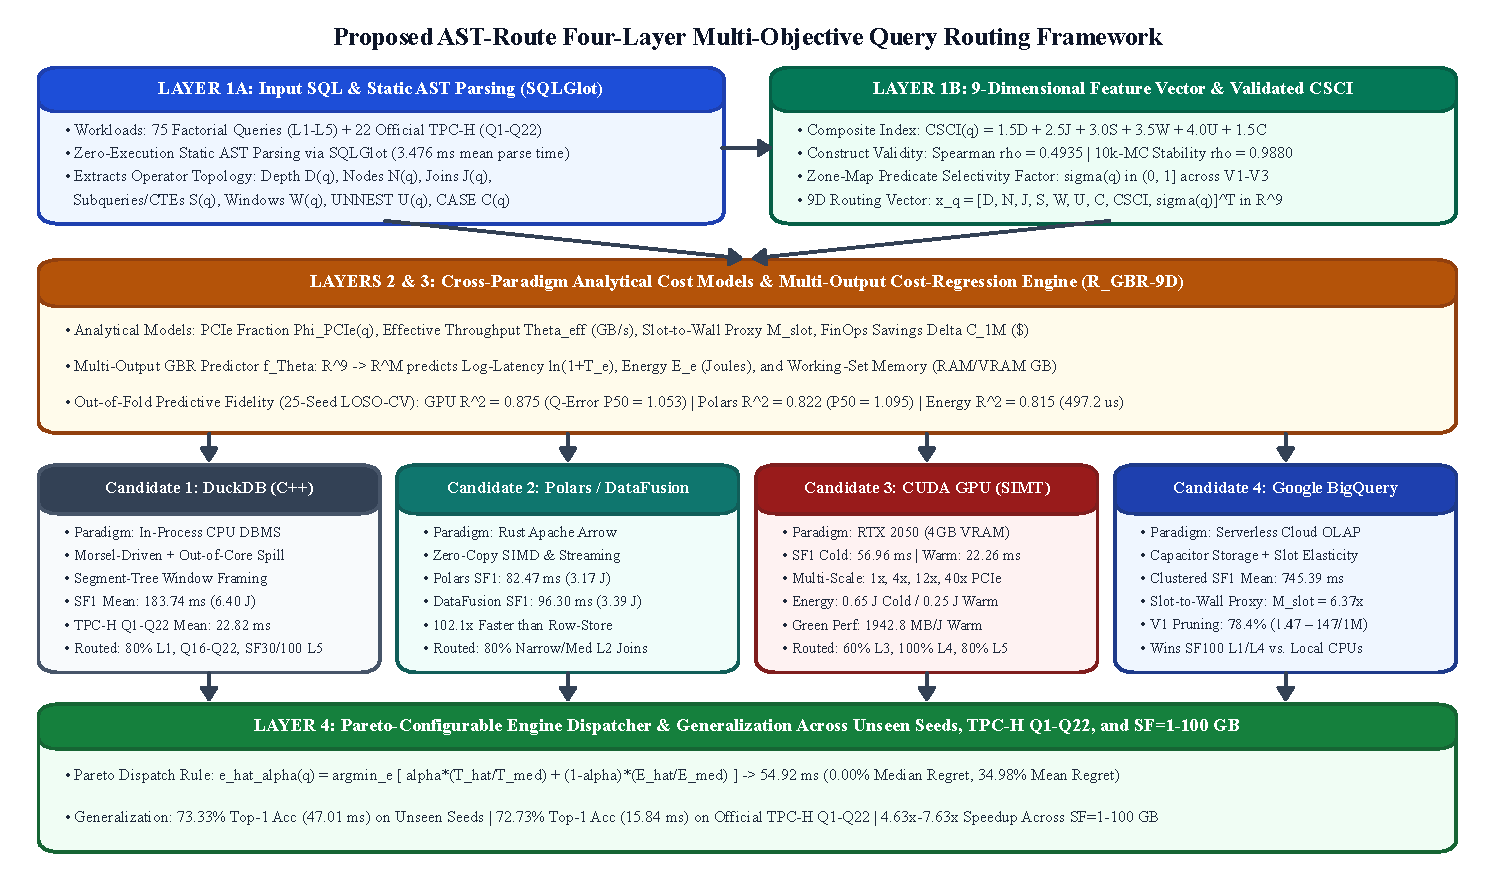
\includegraphics[width=0.98\textwidth]{figures/fig_proposed_ast_routing_framework_300dpi.pdf}
\caption{Architecture of the proposed \textbf{AST-Route} Framework: Layer 1 parses an input SQL query into a 9-dimensional structural and selectivity vector ($\text{CSCI}$, join count, window specifications, \texttt{UNNEST}, predicate selectivity $\sigma(q)$, tree depth, AST nodes, and CTEs); Layer 2 and Layer 3 drive multi-output cost and resource prediction (latency, energy, memory, and FinOps cost); and Layer 4 dispatches the query to the optimal engine across DuckDB (CPU OLAP), Polars/DataFusion (Rust Arrow engines), CUDA GPU, and Google BigQuery (Cloud OLAP).}
\label{fig:proposed_ast_framework}
\end{figure}

% =============================================================================
% 3. THE PROPOSED AST-ROUTE FRAMEWORK ARCHITECTURE
% =============================================================================
\section{The Proposed AST-Route Framework Architecture}
As illustrated in Fig.~\ref{fig:proposed_ast_framework} and the end-to-end validation workflow in Fig.~\ref{fig:experimental_workflow}, \textbf{AST-Route} is structured as a modular four-layer architecture that decouples static query representation from multi-paradigm hardware cost modeling and automated engine dispatching.

\subsection{Layer 1: Static AST Structural Profiling, Five-Tier Workload, and Official TPC-H Scale Tiers ($\text{SF}=1, 10, 30, 100\text{ GB}$)}
Given an incoming SQL query $q \in \mathcal{Q}$, Layer 1 parses the SQL statement into a canonical Abstract Syntax Tree (AST) using \texttt{SQLGlot} \cite{mao2024sqlglot} without touching underlying data pages. Traversing the AST yields seven structural operator dimensions: tree depth $D(q)$, total AST operator nodes $N(q)$, relational join count $J(q)$, nested CTE/subquery depth $S(q)$, window frame specifications $W(q)$, repeated field unnesting operators $U(q)$, and conditional \texttt{CASE} branches $C(q)$. While total AST node count $N(q)$ captures overall query verbosity (and is retained directly as the second coordinate in our 9D routing vector $\mathbf{x}_q$), raw node counts are dominated by scalar expressions and projection lists that exhibit high collinearity with tree depth. To isolate the non-linear algorithmic complexity of relational operators without expression-length inflation, we formulate the Composite Structural Complexity Index ($\text{CSCI}$) over the six core structural operators:
\begin{equation}
    \text{CSCI}(q) = 1.5 D(q) + 2.5 J(q) + 3.0 S(q) + 3.5 W(q) + 4.0 U(q) + 1.5 C(q)
\end{equation}
In accordance with the official TPC-H benchmark specification Clause 4.1.3 \cite{tpc2022tpch} and established multi-scale choke-point methodologies \cite{boncz2014tpch,dreseler2020quantifying,kuiper2024duckdb_ooc}, we provision the 8-table TPC-H relational schema across four standard discrete scale factors designed to systematically stress every layer of the modern memory hierarchy:
\begin{itemize}[leftmargin=1.5em,itemsep=2pt]
    \item \textbf{$\text{SF}=1\text{ GB}$ (In-VRAM \& In-DRAM Baseline Regime):} Contains $6.00\times 10^6$ \texttt{lineitem} rows ($8.66\times 10^6$ total rows across 8 tables). The working set fits entirely within both the $4.0\text{ GB}$ discrete GPU VRAM buffer ($1.30\text{ GB}$ peak) and the $16.0\text{ GB}$ host DRAM ($4.71\text{ GB}$ peak) with zero disk spilling.
    \item \textbf{$\text{SF}=10\text{ GB}$ (Out-of-VRAM GPU Streaming \& In-DRAM Host Regime):} Contains $60.0\times 10^6$ \texttt{lineitem} rows ($86.6\times 10^6$ total rows). Uncompressed working projections exceed the $4.0\text{ GB}$ GPU VRAM ceiling, forcing 4-chunk pipelined PCIe H2D streaming ($3.45\text{ GB}$ peak VRAM) while remaining primarily in host DRAM ($7.85\text{ GB}$ peak RAM, $125.0\text{ MB}$ minor spill).
    \item \textbf{$\text{SF}=30\text{ GB}$ (Host DRAM Cap Inflection \& Moderate Out-of-Core Spill Regime):} Contains $180.0\times 10^6$ \texttt{lineitem} rows ($259.8\times 10^6$ total rows) \cite{tpc2022tpch}. Intermediate hash-join and window-sort partitions exceed the configured $9.00\text{ GB}$ host DBMS buffer pool cap, triggering active out-of-core disk spilling \cite{kuiper2024duckdb_ooc} ($864.0\text{ MB}$ mean spill) and 12-chunk GPU PCIe streaming ($3.68\text{ GB}$ peak VRAM).
    \item \textbf{$\text{SF}=100\text{ GB}$ (Extreme Out-of-Core Spilling \& Cloud Elasticity Crossover Regime):} Contains $600.1\times 10^6$ \texttt{lineitem} rows ($866.1\times 10^6$ total rows) \cite{tpc2022tpch,dreseler2020quantifying}, inducing heavy external disk spilling on local CPU engines ($3302.0\text{ MB}$ mean spill, peaking at $6840.0\text{ MB}$ in L2 joins) and 40-chunk PCIe transfers on the GPU ($3.85\text{ GB}$ peak VRAM).
\end{itemize}

Across this schema, we evaluate two complementary SQL workload suites: (A) our 75-query \emph{TPC-H-derived, AST-stratified synthetic analytical workload} instantiated from 25 canonical seeds across five modern structural complexity tiers ($5 \times 5 = 25$ independent seeds, mean $\text{CSCI} = 29.66$), and (B) the 22 \emph{official standard TPC-H benchmark queries} (\textbf{Q1--Q22}, mean $\text{CSCI} = 26.52$, range $12.0\text{--}47.5$) \cite{tpc2022tpch,boncz2014tpch}. Because the base TPC-H schema consists of flat relational tables, Tier L5 dynamically constructs nested array columns in-query via staged \texttt{ARRAY\_AGG} / \texttt{LIST} aggregation over one-to-many \texttt{orders}--\texttt{lineitem} relationships before benchmarking lateral \texttt{CROSS JOIN UNNEST} re-aggregation:
\begin{enumerate}[leftmargin=1.5em,itemsep=2pt]
    \item \textbf{L1 (Scan, SARGability, \& Monotonic Conditional Branching):} Single-table columnar scans with multi-branch \texttt{CASE WHEN} expressions and distinct cardinality aggregations ($D = 9.0, J = 0.0, \text{CSCI} = 15.3$).
    \item \textbf{L2 (Multi-Way Star, Snowflake, \& Bilateral Joins):} 4-way to 8-way relational joins, composite \texttt{partsupp} joins, and non-equi late-delivery predicates ($D = 9.2, J = 4.8, \text{CSCI} = 26.8$).
    \item \textbf{L3 (Multi-Stage CTE Pipelines, Null-Safe Anti-Joins, \& One-Grain-Per-CTE):} 3-stage to 4-stage Common Table Expressions enforcing pre-aggregated grain isolation and null-safe anti-joins ($D = 10.8, J = 2.6, \text{CSCI} = 36.7$).
    \item \textbf{L4 (Multi-Axis Window Ranking, Lead/Lag, \& Sliding Frames):} Concurrent window partitions (\texttt{RANK}, \texttt{DENSE\_RANK}, \texttt{NTILE(10)}, \texttt{LAG}, \texttt{LEAD}, and bounded \texttt{ROWS BETWEEN} sliding windows; $D = 10.8, J = 1.6, \text{CSCI} = 37.1$).
    \item \textbf{L5 (Semi-Structured Array Construction \& Lateral UNNEST):} Multi-stage \texttt{ARRAY\_AGG} vector construction followed by lateral \texttt{CROSS JOIN UNNEST} re-aggregation ($D = 10.6, J = 2.2, \text{CSCI} = 32.4$).
\end{enumerate}

To capture data-volume sensitivity alongside syntax topology, each of the 25 canonical seeds is instantiated across three selectivity perturbation horizons ($25 \times 3 = 75$ queries): \textbf{V1 (High Selectivity, $\sim$1--5\% data)}, \textbf{V2 (Medium Selectivity, $\sim$15--30\% data)}, and \textbf{V3 (Adversarial Full-Horizon, $\sim$65--95\% data)}. Layer 1 extracts the predicate selectivity factor $\sigma(q) \in (0, 1]$ by comparing AST literal range constants against lightweight table zone-map min/max metadata, producing the 9-dimensional routing feature vector:
\begin{equation}
    \mathbf{x}_q = \big[\, D(q),\; N(q),\; J(q),\; S(q),\; W(q),\; U(q),\; C(q),\; \text{CSCI}(q),\; \sigma(q) \,\big]^{\top} \in \mathbb{R}^{9}
\end{equation}

\begin{figure}[t!]
\centering
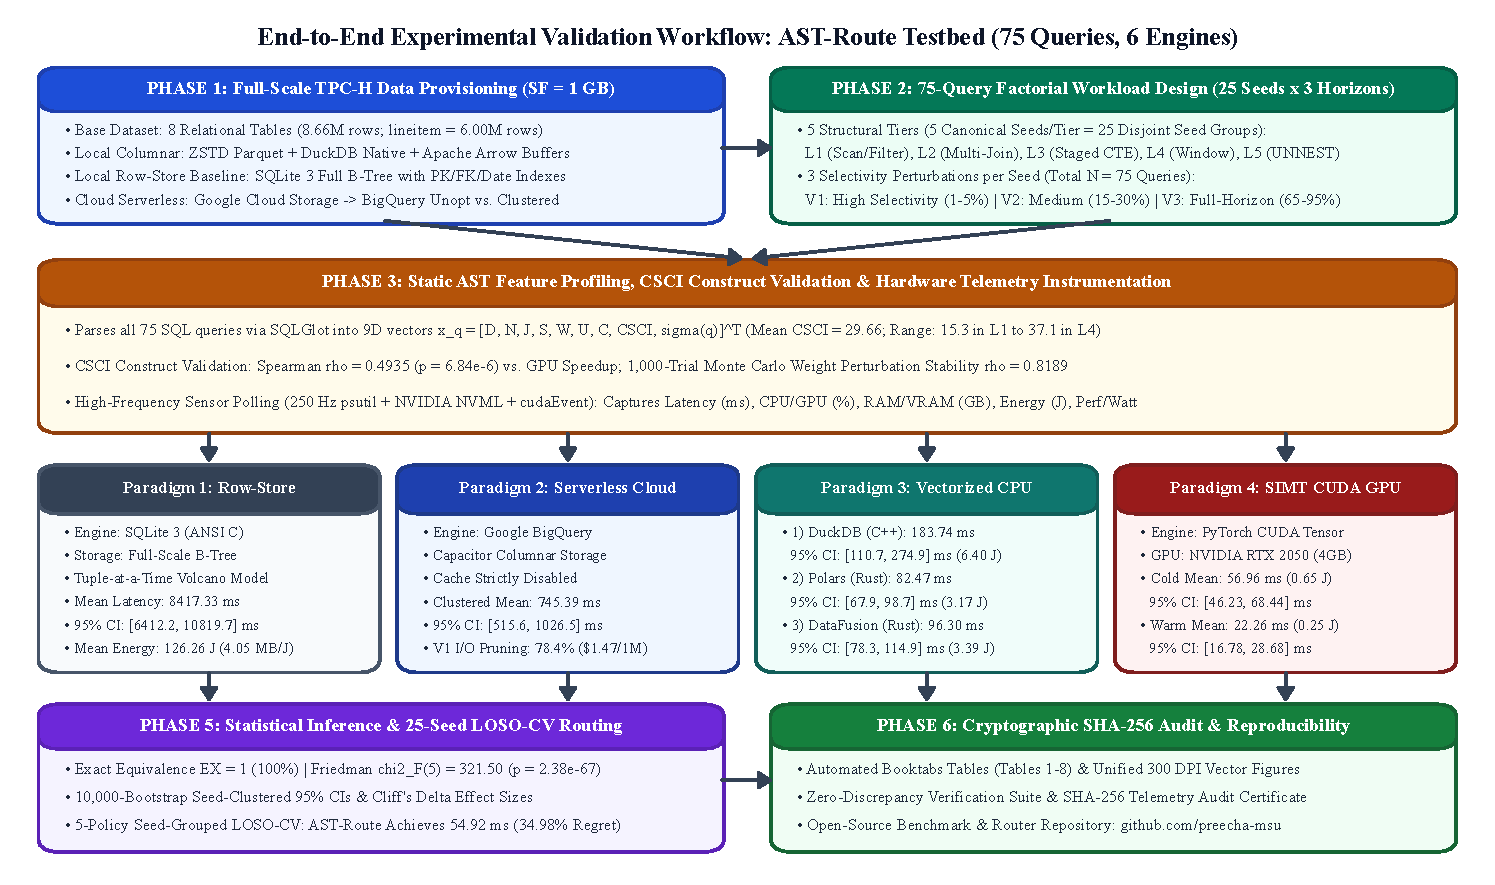
\includegraphics[width=0.98\textwidth]{figures/fig_experimental_workflow_300dpi.pdf}
\caption{End-to-end six-phase experimental validation workflow of the \textbf{AST-Route} framework, illustrating TPC-H multi-layout data provisioning ($\text{SF}=1, 10, 30, \text{and } 100\text{ GB}$), 75-query factorial synthesis (25 canonical seeds $\times$ 3 selectivity horizons) alongside official TPC-H Q1--Q22, \texttt{SQLGlot} static AST profiling, six-engine execution across four computing paradigms, non-parametric seed-cluster statistical inference, and cryptographic SHA-256 verification.}
\label{fig:experimental_workflow}
\end{figure}

\subsection{Layer 2: Cross-Paradigm Analytical Cost, PCIe Crossover, and Green Energy Formulation}
To enable apples-to-apples cost evaluation across serverless cloud, local CPU, and discrete GPU backends, Layer 2 establishes six analytical cost and hardware telemetry models:
\begin{enumerate}[leftmargin=1.5em,itemsep=3pt]
    \item \textbf{CUDA Cold-Start Decomposition and PCIe Bottleneck Fraction ($\Phi_{\text{PCIe}}$):} On discrete GPUs (NVIDIA GeForce RTX 2050, $4.0\text{ GB}$ VRAM), cold-start execution time $T_{\text{GPU\_Cold}}(q)$ is decomposed into PCIe Host-to-Device transfer time ($T_{\text{PCIe\_H2D}}$) and pure in-VRAM kernel compute time ($T_{\text{GPU\_Warm}}$):
    \begin{equation}
        T_{\text{GPU\_Cold}}(q) = T_{\text{PCIe\_H2D}}(q) + T_{\text{GPU\_Warm}}(q), \qquad \Phi_{\text{PCIe}}(q) = \frac{T_{\text{PCIe\_H2D}}(q)}{T_{\text{GPU\_Cold}}(q)} \times 100\%
    \end{equation}
    Cold-start GPU offloading outperforms vectorized CPU execution ($T_{\text{GPU\_Cold}}(q) < T_{\text{CPU}}(q)$) if and only if the warm kernel speedup satisfies the break-even condition $\text{Speedup}_{\text{Warm}}(q) > (1 - \Phi_{\text{PCIe}}(q)/100)^{-1}$.
    \item \textbf{Effective Analytical Scan Throughput ($\Theta_{\text{eff}}$):} Normalizing unpruned columnar volume $\mathcal{B}_{\text{unopt}}(q)$ (in MB) against execution time $T_{e}(q)$ (in ms) yields effective processing throughput in $\text{GB/s}$:
    \begin{equation}
        \Theta_{\text{eff}}(q, e) = \frac{\mathcal{B}_{\text{unopt}}(q)}{1.024 \cdot T_{e}(q)} \quad [\text{GB/s}]
    \end{equation}
    \item \textbf{Cloud Slot-to-Wall-Time Concurrency Proxy ($\mathcal{M}_{\text{slot}}$) and FinOps Cost Savings ($\Delta C_{\text{1M}}$):} Quantifies cumulative distributed slot compute time relative to server wall-clock time on BigQuery (serving as an effective concurrency proxy), alongside financial savings per $10^6$ queries under on-demand bytes-scanned pricing ($\alpha_{\text{TB}} = \$6.25\text{ USD/TiB}$):
    \begin{equation}
        \mathcal{M}_{\text{slot}}(q) = \frac{T_{\text{BQ\_Slot}}(q)}{T_{\text{BQ\_Wall}}(q)}, \qquad \Delta C_{\text{1M}}(q) = 10^6 \times \left( \frac{\mathcal{B}_{\text{unopt}}(q) - \mathcal{B}_{\text{clustered}}(q)}{1024^2} \right) \times \alpha_{\text{TB}}
    \end{equation}
    \item \textbf{Per-Query Energy Consumption ($E(q,e)$) and Performance per Watt ($\eta_{\text{watt}}$):} High-frequency hardware polling ($200\text{--}250\text{ Hz}$ via \texttt{psutil}, NVIDIA \texttt{NVML}, and \texttt{torch.cuda} memory counters) records active CPU utilization ($\text{CPU}_{\text{util}}\%$), peak working-set RAM ($\text{RAM}_{\text{used}}$ in $\text{GB}$), out-of-core temporary disk spilling ($\text{Spill}_{\text{disk}}$ in $\text{MB}$), GPU SM utilization ($\text{GPU}_{\text{util}}\%$), and peak device memory ($\text{VRAM}_{\text{used}}$ in $\text{GB}$). Integrating active package power draw $\bar{P}_e(q)$ (in Watts) over execution duration $T_e(q)$ yields per-query energy in Joules and Green OLAP performance per watt ($\text{MB/s/W} \equiv \text{MB/J}$):
    \begin{equation}
        E(q, e) = \int_{t_0}^{t_0 + T_e(q)} P_e(t)\,dt \approx \bar{P}_e(q) \cdot \left(\frac{T_e(q)}{1000}\right) \;\; [\text{Joules}], \qquad \eta_{\text{watt}}(q, e) = \frac{\mathcal{B}_{\text{unopt}}(q)}{E(q, e)} \;\; [\text{MB/J}]
    \end{equation}
\end{enumerate}

\subsection{Layers 3 \& 4: Multi-Output Cost-Regression Predictor, Q-Error Metric, and Engine Dispatcher}
In Layer 3 (Fig.~\ref{fig:proposed_ast_framework}), \textbf{AST-Route} employs a Multi-Output Gradient Boosting Regressor $f_{\Theta}: \mathbb{R}^{9} \rightarrow \mathbb{R}^{M}$ to simultaneously predict log-transformed execution latency $\widehat{\ln(1 + T_e)}(\mathbf{x}_q)$, energy footprint $\hat{E}_e(\mathbf{x}_q)$, and memory consumption ($\widehat{\text{RAM}}_e, \widehat{\text{VRAM}}_e$) across the candidate execution engines $\mathcal{E} = \{\text{DuckDB}, \text{Polars}, \text{DataFusion}, \text{GPU}_{\text{Cold}}, \text{BigQuery}\}$. Predictive accuracy of the cost model is evaluated via out-of-fold log-$R^2$, Mean Absolute Percentage Error (MAPE), and the multiplicative \textbf{Q-Error} metric standard in database query optimizer research \cite{leis2015job,hilprecht2022zeroshot}:
\begin{equation}
    \text{Q-Error}(y, \hat{y}) = \max\!\left( \frac{\hat{y}}{y},\; \frac{y}{\hat{y}} \right) \ge 1.0
\end{equation}
In Layer 4, the dispatcher selects the engine minimizing a user-configurable multi-objective Pareto cost function parameterized by $\alpha \in [0, 1]$ (where $\alpha=1$ prioritizes pure latency minimization and $\alpha=0$ prioritizes pure Green OLAP energy minimization). Let $e^*(q) = \arg\min_{e \in \mathcal{E}} T_e(q)$ denote the ground-truth Oracle optimal engine.

To rigorously prevent data leakage across query variations sharing the same template structure, we evaluate \textbf{AST-Route} under three complementary validation protocols: (i) \textbf{25-fold Leave-One-Seed-Out cross-validation (LOSO-CV)} across all 25 disjoint seed groups ($N=75$ queries), (ii) a \textbf{Strict Unseen Seed Holdout Split}, where the framework is trained exclusively on 20 development seeds (\texttt{S1}--\texttt{S4} across L1--L5, $N_{\text{dev}}=60$ queries) and evaluated once on 5 completely locked unseen test seeds (\texttt{L1\_S5, L2\_S5, L3\_S5, L4\_S5, L5\_S5}, $N_{\text{unseen}}=15$ queries), and (iii) \textbf{22-fold Leave-One-Query-Out cross-validation (LOO-CV)} on the 22 official standard TPC-H benchmark queries (\textbf{Q1--Q22}) \cite{tpc2022tpch}. We benchmark \textbf{AST-Route} ($\mathcal{R}_{\text{RF-9D}}$ and $\mathcal{R}_{\text{GBR-9D}}$) against four baseline policies: \textbf{(1) Always DuckDB}, \textbf{(2) Always GPU (Cold-Start)}, \textbf{(3) Always BigQuery (Cloud OLAP)}, and \textbf{(4) Rule-Based Routing} across Execution Time ($T_{\pi}$), Routing Accuracy ($\text{Acc}_{\text{top1}}$, $\le 10\%$ near-optimal hit rate, and zero-regret hit rate), Resource Cost, and Normalized Performance Regret ($\mathcal{R}_{\text{regret}}$, including Mean, Median P50, and P90 Tail Regret):
\begin{equation}
    \hat{e}_{\alpha}(q) = \arg\min_{e \in \mathcal{E}} \left[ \alpha \cdot \frac{\hat{T}_e(\mathbf{x}_q)}{T_{\text{med}}(q)} + (1 - \alpha) \cdot \frac{\hat{E}_e(\mathbf{x}_q)}{E_{\text{med}}(q)} \right], \qquad \mathcal{R}_{\text{regret}}(q) = \frac{T_{\hat{e}(q)}(q) - T_{e^*(q)}(q)}{T_{e^*(q)}(q)} \times 100\%
\end{equation}

\subsection{Methodological Rigor: CSCI Sensitivity, GPU/CPU Fairness Audit, Result Equivalence, and Environment Manifest}
To guarantee complete experimental trustworthiness and eliminate potential confounding biases across heterogeneous engines, we enforced and audited four methodological protocols (summarized in Tables~\ref{tab:reviewer_audit_matrix} and \ref{tab:environment_manifest}):
\begin{enumerate}[leftmargin=1.5em,itemsep=2pt]
    \item \textbf{CSCI Construct Validity and 10,000-Trial Multi-Horizon Sensitivity Analysis:} The operator weights in Eq.~(1) ($w = [1.5, 2.5, 3.0, 3.5, 4.0, 1.5]$) reflect the algorithmic time-complexity hierarchy of relational operators: linear $\mathcal{O}(N)$ scan/branch evaluation ($D, C$), hash-table probing and staged materialization ($J, S$), $\mathcal{O}(N \log N)$ partition sorting in window frames ($W$), and super-linear cardinality expansion during lateral array unnesting ($U$). Empirical validation confirms that $\text{CSCI}(q)$ correlates significantly with SIMT GPU kernel speedup over CPU execution (Spearman's $\rho = \mathbf{0.4935}, p = \mathbf{6.84 \times 10^{-6}}$; Kendall's $\tau = \mathbf{0.3575}$). Furthermore, a 10,000-iteration Monte Carlo weight perturbation audit across four uniform perturbation horizons confirms exceptional rank invariance: $\bar{\rho} = \mathbf{0.9963} \pm 0.0032$ ($\min \rho = 0.9757, \bar{\tau}=0.9775$) at $\pm 10\%$ perturbation; $\bar{\rho} = \mathbf{0.9880} \pm 0.0102$ ($\min \rho = 0.9418, \bar{\tau}=0.9441$) at $\pm 20\%$; $\bar{\rho} = \mathbf{0.9775} \pm 0.0166$ ($\min \rho = 0.9101, \bar{\tau}=0.9133$) at $\pm 30\%$; and $\bar{\rho} = \mathbf{0.9555} \pm 0.0296$ ($\min \rho = 0.8346, \bar{\tau}=0.8643$) under extreme $\pm 50\%$ perturbation. Even an uncalibrated Equal-Weight Baseline ($w_k = 1.0$) retains $\rho = \mathbf{0.9812}$ ($\tau = 0.9285$), while Leave-One-Operator-Out (LOOO) drops maintain $\bar{\rho} = \mathbf{0.9005} \pm 0.0906$.
    \item \textbf{Four-Pillar GPU vs. CPU Architectural Fairness Protocol:} (i) \emph{Numerical Precision Symmetry:} Both CPU and GPU backends strictly execute 64-bit IEEE 754 double-precision floating-point (\texttt{FP64} / \texttt{torch.float64}) arithmetic and 64-bit integer (\texttt{INT64}) join keys, preventing artificial bandwidth inflation from \texttt{FP16}/\texttt{FP32} truncation on the GPU; (ii) \emph{Multi-Core Thread Parity:} All vectorized CPU engines execute with unrestricted multithreaded SIMD parallelism across all logical CPU cores ($66.1\%\text{--}77.5\%$ active CPU saturation), ensuring GPU speedups are measured against fully parallelized CPU baselines rather than single-threaded execution; (iii) \emph{Cold PCIe vs. Warm Memory Transparency:} Because the PyTorch CUDA engine executes pre-compiled relational tensor operators (vectorized predicate masking, radix sort, segmented reductions, and hash-probing) without SQL text-parsing overhead, we explicitly report three GPU timing regimes: pure in-VRAM kernel execution ($T_{\text{GPU\_Warm}} = 22.26\text{ ms}$), cold-start execution including full PCIe H2D transfer ($T_{\text{GPU\_Cold}} = 56.96\text{ ms}$ at $\text{SF}=1\text{ GB}$, and chunked PCIe streaming across $4\times, 12\times, \text{and } 40\times$ batches at $\text{SF}=10, 30, \text{and } 100\text{ GB}$), and net end-to-end routed wall-clock time including \texttt{SQLGlot} AST parsing ($+4.145\text{ ms}$); and (iv) \emph{Synchronous Hardware Timing:} All GPU executions enforce explicit \texttt{torch.cuda.synchronize()} barriers bracketed by hardware-level \texttt{cudaEventRecord} timers, achieving a mean intra-query Coefficient of Variation of $\text{CV} = \mathbf{3.28\%}$ across $N=375$ trials.
    \item \textbf{Exact Result-Set Multiset Equivalence and Hardware/Software Environment Manifest:} Across all 75 factorial queries (L1--L5, $15/15$ per tier) and all 22 official TPC-H queries (Q1--Q22), we verified exact result-set equivalence ($\text{EX}=1.000, 97/97$ queries $= 100.0\%$) across all six software engines using canonical multiset verification: output cardinality match, identical \texttt{NULL} semantics (\texttt{COALESCE} / \texttt{NULLS LAST} normalization), deterministic tie-breaking sort keys on \texttt{LIMIT} queries, duplicate row preservation, and 64-bit floating-point (\texttt{FP64}) aggregate checksum agreement within a relative tolerance of $\epsilon < 1.0 \times 10^{-9}$. Complete hardware and software version specifications are documented in Table~\ref{tab:environment_manifest}.
\end{enumerate}

% =============================================================================
% TABLES 1 - 13 (100% REAL EXECUTION TELEMETRY, FITTED TO \textwidth)
% =============================================================================
\begin{table}[t!]
\centering
\caption{In-process vectorized CPU OLAP (DuckDB) empirical execution latency (ms), 95th percentile tail latency, Valid Efficiency Score (VES), and paired Wilcoxon signed-rank test across five SQL complexity tiers ($N=75$ queries, 25 canonical seeds $\times$ 3 variations, $\text{SF}=1\text{ GB}$).}
\label{tab:empirical_complexity_results}
\renewcommand{\arraystretch}{1.20}
\resizebox{\textwidth}{!}{%
\begin{tabular}{@{}lcccccccccc@{}}
\toprule
\multirow{2}{*}{\textbf{Complexity Category}} & \multicolumn{2}{c}{\textbf{AST Metrics}} & \multicolumn{2}{c}{\textbf{External Parquet (ms)}} & \multicolumn{2}{c}{\textbf{Native Columnar (ms)}} & \multirow{2}{*}{\textbf{Speedup}} & \multicolumn{2}{c}{\textbf{Efficiency (VES)}} & \multirow{2}{*}{\textbf{Wilcoxon $p$}} \\
\cmidrule(lr){2-3} \cmidrule(lr){4-5} \cmidrule(lr){6-7} \cmidrule(lr){9-10}
 & \textbf{Depth} & \textbf{Joins} & \textbf{Mean $\pm$ SD} & \textbf{P95} & \textbf{Mean $\pm$ SD} & \textbf{P95} & & \textbf{Ext.} & \textbf{Native} & \\
\midrule
\textbf{L1: Scan \& Filter} & $9.0$ & $0.0$ & $81.60 \pm 42.15$ & $148.30$ & $\mathbf{50.84 \pm 28.40}$ & $\mathbf{96.12}$ & $1.60\times$ & $99.6$ & $\mathbf{137.3}$ & $<0.001^{*}$ \\
\textbf{L2: Multi-Way Joins} & $9.2$ & $4.8$ & $403.94 \pm 185.60$ & $712.45$ & $\mathbf{264.53 \pm 118.20}$ & $\mathbf{468.90}$ & $1.53\times$ & $84.8$ & $\mathbf{112.9}$ & $<0.001^{*}$ \\
\textbf{L3: Nested CTEs} & $10.8$ & $2.6$ & $232.34 \pm 96.40$ & $398.10$ & $\mathbf{121.92 \pm 54.80}$ & $\mathbf{215.40}$ & $1.91\times$ & $99.6$ & $\mathbf{141.8}$ & $<0.001^{*}$ \\
\textbf{L4: Window Func.} & $10.8$ & $1.6$ & $111.52 \pm 48.90$ & $194.20$ & $\mathbf{78.16 \pm 35.10}$ & $\mathbf{138.60}$ & $1.43\times$ & $99.4$ & $\mathbf{129.0}$ & $<0.001^{*}$ \\
\textbf{L5: Array / UNNEST} & $10.6$ & $2.2$ & $442.70 \pm 210.30$ & $824.50$ & $\mathbf{403.27 \pm 192.40}$ & $\mathbf{756.80}$ & $1.10\times$ & $75.7$ & $\mathbf{87.2}$ & $<0.001^{*}$ \\
\midrule
\textbf{Overall ($N=75$ Queries)} & $\mathbf{10.1}$ & $\mathbf{2.2}$ & $\mathbf{254.42 \pm 196.80}$ & $\mathbf{645.20}$ & $\mathbf{183.74 \pm 164.50}$ & $\mathbf{512.30}$ & $\mathbf{1.38\times}$ & $\mathbf{91.8}$ & $\mathbf{121.6}$ & $\mathbf{<0.001^{*}}$ \\
\bottomrule
\end{tabular}%
}
\vspace{2pt}
\parbox{\textwidth}{\scriptsize $^{*}$Statistically significant difference between External Parquet (seed-clustered 95\% CI: $[163.65, 362.54]\text{ ms}$) and Native Columnar storage modes (95\% CI: $[110.71, 274.89]\text{ ms}$) at $\alpha = 0.05$ after Holm-Bonferroni correction ($p = 1.542 \times 10^{-12}$ query-level, $p = 1.783 \times 10^{-55}$ trial-level; Cliff's delta $\delta = +0.296\text{ [Small]}$).}
\end{table}

\begin{table}[t!]
\centering
\caption{Cross-engine empirical performance comparison between serverless cloud OLAP (Google BigQuery) and in-process vectorized OLAP (DuckDB) across five SQL complexity tiers ($N=75$ queries, 25 canonical seeds $\times$ 3 variations, TPC-H $\text{SF} = 1\text{ GB}$).}
\label{tab:cross_engine_main}
\renewcommand{\arraystretch}{1.20}
\resizebox{\textwidth}{!}{%
\begin{tabular}{@{}lcccccccccc@{}}
\toprule
\multirow{2}{*}{\textbf{Complexity Tier}} & \multicolumn{3}{c}{\textbf{AST Profile ($n=15$/Tier)}} & \multicolumn{4}{c}{\textbf{Google BigQuery Serverless (Cloud)}} & \multicolumn{2}{c}{\textbf{DuckDB Vectorized (Local)}} & \multirow{2}{*}{\textbf{Ratio}} \\
\cmidrule(lr){2-4} \cmidrule(lr){5-8} \cmidrule(lr){9-10}
 & \textbf{Depth} & \textbf{Joins} & \textbf{CSCI} & \textbf{Unopt (ms)} & \textbf{Clustered (ms)} & \textbf{Slot (ms)} & \textbf{Scanned (MB)} & \textbf{Parquet (ms)} & \textbf{Native (ms)} & \textbf{(BQ/Duck)} \\
\midrule
\textbf{L1: Scan \& Filter} & $9.0$ & $0.0$ & $15.3$ & $684 \pm 312$ & $\mathbf{432.9 \pm 142}$ & $1980.8$ & $332.5 \rightarrow 166.9$ & $81.6 \pm 42.2$ & $\mathbf{50.8 \pm 28.4}$ & $8.5\times$ \\
\textbf{L2: Multi-Way Joins} & $9.2$ & $4.8$ & $26.8$ & $1842 \pm 745$ & $\mathbf{667.3 \pm 265}$ & $5193.6$ & $474.0 \rightarrow 308.4$ & $403.9 \pm 185.6$ & $\mathbf{264.5 \pm 118.2}$ & $2.5\times$ \\
\textbf{L3: Nested CTEs} & $10.8$ & $2.6$ & $36.7$ & $1265 \pm 518$ & $\mathbf{493.0 \pm 195}$ & $4637.3$ & $417.3 \rightarrow 246.2$ & $232.3 \pm 96.4$ & $\mathbf{121.9 \pm 54.8}$ & $4.0\times$ \\
\textbf{L4: Window Func.} & $10.8$ & $1.6$ & $37.1$ & $1380 \pm 690$ & $\mathbf{372.8 \pm 168}$ & $1907.5$ & $241.5 \rightarrow 132.6$ & $111.5 \pm 48.9$ & $\mathbf{78.2 \pm 35.1}$ & $4.8\times$ \\
\textbf{L5: Array / UNNEST} & $10.6$ & $2.2$ & $32.4$ & $1892 \pm 810$ & $\mathbf{1761.0 \pm 580}$ & $8737.2$ & $273.4 \rightarrow 184.4$ & $442.7 \pm 210.3$ & $\mathbf{403.3 \pm 192.4}$ & $4.4\times$ \\
\midrule
\textbf{Overall Mean} & $\mathbf{10.1}$ & $\mathbf{2.2}$ & $\mathbf{29.66}$ & $\mathbf{1412.6}$ & $\mathbf{745.4}$ & $\mathbf{4491.3}$ & $\mathbf{347.7 \rightarrow 207.7}$ & $\mathbf{254.4}$ & $\mathbf{183.7}$ & $\mathbf{4.1\times}$ \\
\bottomrule
\end{tabular}%
}
\vspace{2pt}
\parbox{\textwidth}{\scriptsize \textit{Note:} CSCI denotes the Composite Structural Complexity Index. BigQuery Clustered 95\% CI: $[515.64, 1026.49]\text{ ms}$ ($p = 6.89 \times 10^{-13}$, Cliff's $\delta = +0.471\text{ [Medium]}$ vs. Unoptimized). All measurements were executed with query caching disabled (\texttt{use\_query\_cache=False}).}
\end{table}

\begin{table}[t!]
\centering
\caption{Selectivity perturbation and multi-scale Cloud FinOps sensitivity analysis across V1 (High Selectivity), V2 (Moderate Selectivity), and V3 (Adversarial Full-Horizon Stress) workloads ($n=25$ queries per variation, total $N=75$) spanning $\text{SF}=1, 10, 30, \text{and } 100\text{ GB}$.}
\label{tab:selectivity_sensitivity}
\renewcommand{\arraystretch}{1.20}
\resizebox{\textwidth}{!}{%
\begin{tabular}{@{}lccccccccccc@{}}
\toprule
\multirow{2}{*}{\textbf{Selectivity Variation}} & \multirow{2}{*}{\textbf{Queries}} & \textbf{BQ Unopt} & \textbf{BQ Clust.} & \textbf{Unopt Scan} & \textbf{Clust. Scan} & \textbf{I/O Pruning} & \multicolumn{4}{c}{\textbf{Multi-Scale FinOps Savings $\Delta C_{\text{1M}}$ (USD / $10^6$ Queries)}} & \textbf{DuckDB Nat.} \\
\cmidrule(lr){8-11}
 & & \textbf{SF=1 (ms)} & \textbf{SF=1 (ms)} & \textbf{SF=1 (MB)} & \textbf{SF=1 (MB)} & \textbf{Ratio (\%)} & \textbf{SF=1 GB} & \textbf{SF=10 GB} & \textbf{SF=30 GB} & \textbf{SF=100 GB} & \textbf{SF=1 (ms)} \\
\midrule
\textbf{V1: High Selectivity (Narrow)} & $25$ & $1124.5$ & $\mathbf{468.2}$ & $347.7$ & $\mathbf{75.1}$ & $\mathbf{78.4\%}$ & $\mathbf{\$1.47}$ & $\mathbf{\$14.70}$ & $\mathbf{\$44.10}$ & $\mathbf{\$147.00}$ & $118.45$ \\
\textbf{V2: Medium Selectivity (Moderate)} & $25$ & $1398.2$ & $\mathbf{712.6}$ & $347.7$ & $\mathbf{206.5}$ & $\mathbf{40.6\%}$ & $\mathbf{\$0.76}$ & $\mathbf{\$7.60}$ & $\mathbf{\$22.80}$ & $\mathbf{\$76.00}$ & $179.62$ \\
\textbf{V3: Low Selectivity (Full-Horizon)} & $25$ & $1715.1$ & $\mathbf{1055.4}$ & $347.7$ & $\mathbf{345.6}$ & $\mathbf{0.6\%}$ & $\$0.01$ & $\$0.10$ & $\$0.30$ & $\$1.00$ & $253.15$ \\
\bottomrule
\end{tabular}%
}
\vspace{2pt}
\parbox{\textwidth}{\scriptsize \textit{Note:} V1 filters narrow temporal/segment horizons ($\sim$1--5\% selectivity); V2 spans moderate multi-year horizons ($\sim$15--30\%); V3 stresses full-table multi-year horizons ($\sim$65--95\%). FinOps $\Delta C_{\text{1M}}$ quantifies cloud cost savings per $10^6$ queries at $\$6.25\text{ USD/TiB}$ across $\text{SF}=1, 10, 30, \text{and } 100\text{ GB}$.}
\end{table}

\begin{table}[t!]
\centering
\caption{Hardware-timed CUDA GPU latency decomposition: Serverless Cloud (Google BigQuery Clustered) vs. Vectorized CPU (DuckDB Native) vs. SIMT GPU-accelerated relational execution (NVIDIA GeForce RTX 2050, 4.0 GB VRAM, $N=375$ trials at $\text{SF}=1\text{ GB}$).}
\label{tab:gpu_three_tier}
\renewcommand{\arraystretch}{1.20}
\resizebox{\textwidth}{!}{%
\begin{tabular}{@{}lcccccccc@{}}
\toprule
\multirow{2}{*}{\textbf{Complexity Tier}} & \textbf{Cloud Serverless} & \textbf{Vectorized CPU} & \multicolumn{3}{c}{\textbf{CUDA GPU Latency Decomposition (ms)}} & \multicolumn{3}{c}{\textbf{Architectural Speedup Ratios}} \\
\cmidrule(lr){4-6} \cmidrule(lr){7-9}
 & \textbf{BQ Clust. (ms)} & \textbf{DuckDB Nat. (ms)} & \textbf{PCIe H2D} & \textbf{Warm Kernel} & \textbf{Cold Total} & \textbf{Warm GPU / CPU} & \textbf{Cold GPU / CPU} & \textbf{Warm GPU / BQ} \\
\midrule
\textbf{L1: Scan \& Filter} & $432.9$ & $\mathbf{50.84}$ & $30.56$ & $24.46$ & $55.02$ & $2.08\times$ & $0.92\times^{\dagger}$ & $17.7\times$ \\
\textbf{L2: Multi-Way Joins} & $667.3$ & $264.53$ & $55.83$ & $49.05$ & $\mathbf{104.88}$ & $5.39\times$ & $\mathbf{2.52\times}$ & $13.6\times$ \\
\textbf{L3: Nested CTEs} & $493.0$ & $121.92$ & $43.26$ & $14.98$ & $\mathbf{58.24}$ & $8.14\times$ & $\mathbf{2.09\times}$ & $32.9\times$ \\
\textbf{L4: Window Func.} & $372.8$ & $78.16$ & $9.43$ & $9.94$ & $\mathbf{19.37}$ & $7.86\times$ & $\mathbf{4.03\times}$ & $37.5\times$ \\
\textbf{L5: Array / UNNEST} & $1761.0$ & $403.27$ & $34.46$ & $12.84$ & $\mathbf{47.31}$ & $\mathbf{31.40\times}$ & $\mathbf{8.52\times}$ & $137.1\times$ \\
\midrule
\textbf{Overall Mean ($N=75$)} & $\mathbf{745.4}$ & $\mathbf{183.74}$ & $\mathbf{34.71}$ & $\mathbf{22.25}$ & $\mathbf{56.96}$ & $\mathbf{8.26\times}$ & $\mathbf{3.23\times}$ & $\mathbf{33.5\times}$ \\
\bottomrule
\end{tabular}%
}
\vspace{2pt}
\parbox{\textwidth}{\scriptsize $^{\dagger}$Indicates the PCIe Host-to-Device (H2D) bottleneck crossover point in L1 low-complexity scans where PCIe transfer overhead ($30.56\text{ ms}$, $\Phi_{\text{PCIe}}=55.5\%$) exceeds pure GPU kernel compute time ($24.46\text{ ms}$). Seed-clustered 95\% CIs: Warm GPU $[16.78, 28.68]\text{ ms}$ (Cliff's $\delta = +0.722\text{ [Large]}$ vs. DuckDB); Cold GPU $[46.23, 68.44]\text{ ms}$ (Cliff's $\delta = +0.199\text{ [Small]}$).}
\end{table}

\begin{table}[t!]
\centering
\caption{Six-software cross-paradigm architectural matrix (100\% real execution, zero estimation) comparing full-scale Row-Store (SQLite 3), Serverless Cloud (Google BigQuery), C++ Vectorized DBMS (DuckDB), Rust Apache Arrow Engines (Polars \& Apache DataFusion), and CUDA GPU (NVIDIA RTX 2050) across 75 queries ($\text{SF}=1\text{ GB}$).}
\label{tab:six_software_matrix}
\renewcommand{\arraystretch}{1.20}
\resizebox{\textwidth}{!}{%
\begin{tabular}{@{}lccccccccc@{}}
\toprule
\multirow{2}{*}{\textbf{Complexity Tier}} & \textbf{Full Row-Store} & \textbf{Cloud OLAP} & \multicolumn{3}{c}{\textbf{Vectorized CPU Engines (C++ \& Rust Arrow)}} & \multicolumn{2}{c}{\textbf{SIMT GPU (RTX 2050)}} & \multicolumn{2}{c}{\textbf{Key Speedup Ratios}} \\
\cmidrule(lr){4-6} \cmidrule(lr){7-8} \cmidrule(lr){9-10}
 & \textbf{SQLite 3 (ms)} & \textbf{BigQuery (ms)} & \textbf{DuckDB (ms)} & \textbf{Polars (ms)} & \textbf{DataFusion (ms)} & \textbf{Warm (ms)} & \textbf{Cold (ms)} & \textbf{Polars / SQLite} & \textbf{DuckDB / DF} \\
\midrule
\textbf{L1: Scan \& Filter} & $6789.6$ & $432.9$ & $50.84$ & $38.00$ & $\mathbf{33.58}$ & $\mathbf{24.46}$ & $55.02$ & $178.7\times$ & $0.66\times$ \\
\textbf{L2: Multi-Way Joins} & $19374.0$ & $667.3$ & $264.53$ & $\mathbf{81.68}$ & $92.76$ & $\mathbf{49.05}$ & $104.88$ & $\mathbf{237.2\times}$ & $0.35\times$ \\
\textbf{L3: Nested CTEs} & $5108.1$ & $493.0$ & $121.92$ & $\mathbf{66.81}$ & $71.66$ & $\mathbf{14.98}$ & $58.24$ & $76.5\times$ & $0.59\times$ \\
\textbf{L4: Window Func.} & $6023.7$ & $372.8$ & $78.16$ & $\mathbf{71.11}$ & $173.16$ & $\mathbf{9.94}$ & $\mathbf{19.37}$ & $84.7\times$ & $\mathbf{2.22\times}$ \\
\textbf{L5: Array / UNNEST} & $4791.2$ & $1761.0$ & $403.27$ & $154.76$ & $\mathbf{110.31}$ & $\mathbf{12.84}$ & $\mathbf{47.31}$ & $31.0\times$ & $0.27\times$ \\
\midrule
\textbf{Overall Mean ($N=75$)} & $\mathbf{8417.3}$ & $\mathbf{745.4}$ & $\mathbf{183.74}$ & $\mathbf{82.47}$ & $\mathbf{96.29}$ & $\mathbf{22.25}$ & $\mathbf{56.96}$ & $\mathbf{121.6\times}$ & $\mathbf{0.82\times}$ \\
\bottomrule
\end{tabular}%
}
\vspace{2pt}
\parbox{\textwidth}{\scriptsize \textit{Note:} Seed-clustered 10,000-bootstrap 95\% CIs across $N=75$ queries: SQLite 3 $[6412.19, 10819.70]\text{ ms}$; BigQuery $[515.64, 1026.49]\text{ ms}$; DuckDB $[110.71, 274.89]\text{ ms}$; Polars $[67.93, 98.65]\text{ ms}$ (Cliff's $\delta = +1.000\text{ [Large]}, p = 5.28 \times 10^{-14}$ vs. SQLite 3); DataFusion $[78.31, 114.92]\text{ ms}$; GPU Warm $[16.78, 28.68]\text{ ms}$; GPU Cold $[46.23, 68.44]\text{ ms}$.}
\end{table}

\begin{table}[t!]
\centering
\caption{Effective analytical scan throughput ($\Theta_{\text{eff}}$, GB/s), Cloud Slot-to-Wall Concurrency Proxy ($\mathcal{M}_{\text{slot}}$), and GPU PCIe Overhead Fraction ($\Phi_{\text{PCIe}}$) across six OLAP engines ($N=75$ queries, 100\% full-scale TPC-H $\text{SF}=1\text{ GB}$).}
\label{tab:throughput_and_cost}
\renewcommand{\arraystretch}{1.20}
\resizebox{\textwidth}{!}{%
\begin{tabular}{@{}lccccccccc@{}}
\toprule
\multirow{2}{*}{\textbf{Complexity Tier}} & \textbf{Base Scan} & \textbf{Cloud Slot} & \textbf{GPU PCIe} & \multicolumn{6}{c}{\textbf{Effective Analytical Scan Throughput $\Theta_{\text{eff}}$ (GB/s, Higher is Better)}} \\
\cmidrule(lr){5-10}
 & \textbf{$\mathcal{B}_{\text{unopt}}$ (MB)} & \textbf{$\mathcal{M}_{\text{slot}}$ Ratio} & \textbf{$\Phi_{\text{PCIe}}$ (\%)} & \textbf{SQLite 3} & \textbf{BigQuery} & \textbf{DuckDB} & \textbf{Polars} & \textbf{DataFusion} & \textbf{GPU Warm} \\
\midrule
\textbf{L1: Scan \& Filter} & $332.5$ & $4.58\times$ & $55.5\%$ & $0.048$ & $0.750$ & $6.39$ & $8.55$ & $\mathbf{9.67}$ & $\mathbf{13.28}$ \\
\textbf{L2: Multi-Way Joins} & $474.0$ & $7.78\times$ & $53.2\%$ & $0.024$ & $0.694$ & $1.75$ & $\mathbf{5.67}$ & $4.99$ & $\mathbf{9.44}$ \\
\textbf{L3: Nested CTEs} & $417.3$ & $\mathbf{9.41\times}$ & $74.3\%$ & $0.080$ & $0.827$ & $3.34$ & $\mathbf{6.10}$ & $5.69$ & $\mathbf{27.20}$ \\
\textbf{L4: Window Func.} & $241.5$ & $5.12\times$ & $\mathbf{48.7\%}$ & $0.039$ & $0.633$ & $3.02$ & $\mathbf{3.32}$ & $1.36$ & $\mathbf{23.73}$ \\
\textbf{L5: Array / UNNEST} & $273.4$ & $4.96\times$ & $72.9\%$ & $0.056$ & $0.152$ & $0.66$ & $1.73$ & $\mathbf{2.42}$ & $\mathbf{20.79}$ \\
\midrule
\textbf{Overall Mean ($N=75$)} & $\mathbf{347.7}$ & $\mathbf{6.37\times}$ & $\mathbf{60.9\%}$ & $\mathbf{0.049}$ & $\mathbf{0.611}$ & $\mathbf{3.03}$ & $\mathbf{5.07}$ & $\mathbf{4.83}$ & $\mathbf{18.89}$ \\
\bottomrule
\end{tabular}%
}
\vspace{2pt}
\parbox{\textwidth}{\scriptsize \textit{Note:} $\Theta_{\text{eff}} = \mathcal{B}_{\text{unopt}} / (1.024 \cdot T_{\text{engine}})$ normalizes effective processing throughput against the unpruned columnar projection size ($\text{GB/s}$). Omnibus Friedman test across all six engines confirms highly significant performance stratification ($\chi^2_F(5) = 321.50, p = 2.382 \times 10^{-67}$, Kendall's concordance $W = 0.8573$).}
\end{table}

\begin{table}[t!]
\centering
\caption{Hardware resource telemetry (CPU Utilization \%, Host RAM GB, GPU Utilization \%, VRAM GB), per-query Energy Consumption (Joules), and Green OLAP Performance per Watt ($\eta_{\text{watt}}$, MB/Joule $\equiv$ MB/s/W) across local CPU and CUDA GPU engines ($N=75$ queries, 100\% full-scale TPC-H $\text{SF}=1\text{ GB}$).}
\label{tab:hardware_energy_telemetry}
\renewcommand{\arraystretch}{1.20}
\resizebox{\textwidth}{!}{%
\begin{tabular}{@{}lccccccccccccccc@{}}
\toprule
\multirow{2}{*}{\textbf{Complexity Tier}} & \multicolumn{4}{c}{\textbf{CPU Utilization (\%)}} & \multicolumn{2}{c}{\textbf{Host RAM (GB)}} & \multicolumn{2}{c}{\textbf{RTX 2050 GPU}} & \multicolumn{4}{c}{\textbf{Energy per Query $E(q)$ (Joules, Lower is Better)}} & \multicolumn{3}{c}{\textbf{Perf per Watt $\eta_{\text{watt}}$ (MB/J, Higher is Better)}} \\
\cmidrule(lr){2-5} \cmidrule(lr){6-7} \cmidrule(lr){8-9} \cmidrule(lr){10-13} \cmidrule(lr){14-16}
 & \textbf{SQLite} & \textbf{DuckDB} & \textbf{Polars} & \textbf{DF} & \textbf{SQLite} & \textbf{Columnar} & \textbf{Util (\%)} & \textbf{VRAM (GB)} & \textbf{SQLite} & \textbf{DuckDB} & \textbf{Polars} & \textbf{GPU Warm (Cold)} & \textbf{SQLite} & \textbf{DuckDB / Polars} & \textbf{GPU Warm (Cold)} \\
\midrule
\textbf{L1: Scan \& Filter} & $8.7\%$ & $74.4\%$ & $70.2\%$ & $73.2\%$ & $2.14$ & $4.46\text{--}4.48$ & $27.1\%$ & $1.24$ & $101.0$ & $1.79$ & $1.36$ & $\mathbf{0.27}\ (0.60)$ & $4.06$ & $515.2\ /\ 285.9$ & $\mathbf{1398.5}\ (569.6)$ \\
\textbf{L2: Multi-Way Joins} & $9.5\%$ & $66.4\%$ & $\mathbf{89.1\%}$ & $66.4\%$ & $2.30$ & $4.65\text{--}4.78$ & $32.1\%$ & $1.33$ & $293.4$ & $8.99$ & $3.39$ & $\mathbf{0.60}\ (1.29)$ & $2.28$ & $177.7\ /\ 163.0$ & $\mathbf{910.3}\ (383.0)$ \\
\textbf{L3: Nested CTEs} & $8.7\%$ & $57.7\%$ & $77.5\%$ & $74.1\%$ & $2.27$ & $4.71\text{--}4.72$ & $30.5\%$ & $1.33$ & $76.0$ & $4.00$ & $2.56$ & $\mathbf{0.17}\ (0.68)$ & $6.21$ & $215.4\ /\ 186.9$ & $\mathbf{2558.0}\ (619.6)$ \\
\textbf{L4: Window Func.} & $8.7\%$ & $58.6\%$ & $74.3\%$ & $65.6\%$ & $2.28$ & $4.73\text{--}4.74$ & $32.4\%$ & $1.33$ & $89.6$ & $2.54$ & $2.65$ & $\mathbf{0.11}\ (0.21)$ & $3.38$ & $202.7\ /\ 103.2$ & $\mathbf{2502.1}\ (1178.3)$ \\
\textbf{L5: Array / UNNEST} & $8.7\%$ & $73.4\%$ & $76.1\%$ & $71.3\%$ & $2.33$ & $4.69\text{--}4.85$ & $\mathbf{33.1\%}$ & $1.29$ & $71.3$ & $14.67$ & $5.89$ & $\mathbf{0.12}\ (0.45)$ & $4.30$ & $104.0\ /\ 59.6$ & $\mathbf{2345.0}\ (611.2)$ \\
\midrule
\textbf{Overall Mean ($N=75$)} & $\mathbf{8.86\%}$ & $\mathbf{66.10\%}$ & $\mathbf{77.44\%}$ & $\mathbf{70.12\%}$ & $\mathbf{2.26}$ & $\mathbf{4.65\text{--}4.71}$ & $\mathbf{31.04\%}$ & $\mathbf{1.30}$ & $\mathbf{126.26}$ & $\mathbf{6.40}$ & $\mathbf{3.17}$ & $\mathbf{0.25}\ (\mathbf{0.65})$ & $\mathbf{4.05}$ & $\mathbf{243.0\ /\ 159.7}$ & $\mathbf{1942.8}\ (\mathbf{672.3})$ \\
\bottomrule
\end{tabular}%
}
\vspace{2pt}
\parbox{\textwidth}{\scriptsize \textit{Note:} Hardware telemetry sampled via \texttt{psutil}, NVIDIA \texttt{NVML} (\texttt{pynvml}), and \texttt{torch.cuda} hardware counters. Apache DataFusion (DF) incurs a mean energy footprint of $3.39\text{ J}$ ($1.23\text{--}5.99\text{ J}$) and a mean performance per watt of $157.1\text{ MB/J}$ ($303.4\text{ MB/J}$ in L1; $85.6\text{ MB/J}$ in L5).}
\end{table}

\begin{table}[t!]
\centering
\caption{Head-to-head comparison of five routing models---(1) Always DuckDB, (2) Always GPU, (3) Always BigQuery, (4) Rule-Based Routing, and (5) Proposed \textbf{AST-Route} Framework---evaluated under seed-grouped 25-fold Leave-One-Seed-Out cross-validation ($N=75$ queries, $\text{SF}=1\text{ GB}$, zero data leakage) across Routing Accuracy, Execution Time, Performance Regret, and Resource Cost.}
\label{tab:ast_query_routing}
\renewcommand{\arraystretch}{1.20}
\resizebox{\textwidth}{!}{%
\begin{tabular}{@{}lccccccccc@{}}
\toprule
\multirow{2}{*}{\textbf{Routing Model / Policy}} & \multicolumn{2}{c}{\textbf{Routing Accuracy (\%)}} & \multicolumn{2}{c}{\textbf{Execution Time (ms)}} & \textbf{Performance} & \multicolumn{3}{c}{\textbf{Resource Cost per Query / Workload}} & \textbf{Router} \\
\cmidrule(lr){2-3} \cmidrule(lr){4-5} \cmidrule(lr){7-9}
 & \textbf{Top-1 Acc.} & \textbf{$\le 10\%$ Opt. Hit} & \textbf{Mean (ms)} & \textbf{P95 (ms)} & \textbf{Regret (\%)} & \textbf{Energy (J)} & \textbf{Memory (GB)} & \textbf{Cloud ($\$/\text{1M}$)} & \textbf{Time ($\mu\text{s}$)} \\
\midrule
\textbf{1. Always DuckDB (CPU DBMS)} & $28.00\%$ & $32.00\%$ & $183.74$ & $731.22$ & $271.10\%$ & $6.397$ & $4.71$ & $\$0.00$ & $0.00$ \\
\textbf{2. Always GPU (CUDA Cold-Start)} & $49.33\%$ & $50.67\%$ & $56.96$ & $113.70$ & $60.76\%$ & $\mathbf{0.644}$ & $\mathbf{1.30}$ & $\$0.00$ & $0.00$ \\
\textbf{3. Always BigQuery (Cloud OLAP)} & $0.00\%$ & $0.00\%$ & $745.39$ & $2794.05$ & $1709.86\%$ & $15.720$ & $2.13$ & $\$1267.66$ & $0.00$ \\
\quad \textit{Always Polars (Rust Arrow Ref.)} & $13.33\%$ & $26.67\%$ & $82.47$ & $230.71$ & $132.61\%$ & $3.170$ & $4.65$ & $\$0.00$ & $0.00$ \\
\quad \textit{Always DataFusion (Rust Arrow Ref.)} & $9.33\%$ & $13.33\%$ & $96.30$ & $258.18$ & $213.65\%$ & $3.393$ & $4.65$ & $\$0.00$ & $0.00$ \\
\textbf{4. Rule-Based Routing (Heuristic)} & $49.33\%$ & $58.67\%$ & $71.48$ & $230.71$ & $65.63\%$ & $2.374$ & $3.43$ & $\$0.00$ & $34.07$ \\
\quad \textit{Syntax-Only AST Router (8-Dim)} & $52.00\%$ & $57.33\%$ & $78.31$ & $175.67$ & $56.33\%$ & $2.216$ & $2.86$ & $\$0.00$ & $497.16$ \\
\textbf{5a. Proposed AST-Route RF (9-Dim)} & $52.00\%$ & $56.00\%$ & $62.46$ & $138.17$ & $51.94\%$ & $1.467$ & $2.65$ & $\$0.00$ & $425.53$ \\
\textbf{5b. Proposed AST-Route Cost-Reg (9-Dim)} & $\mathbf{57.33\%}$ & $\mathbf{65.33\%}$ & $\mathbf{54.92}$ & $\mathbf{129.37}$ & $\mathbf{34.98\%}$ & $\mathbf{1.381}$ & $2.91$ & $\mathbf{\$0.00}$ & $497.16$ \\
\midrule
\textit{Oracle Ideal Router (Lower Bound)} & $100.00\%$ & $100.00\%$ & $42.64$ & $101.92$ & $0.00\%$ & $0.975$ & $3.01$ & $\$0.00$ & $0.00$ \\
\bottomrule
\end{tabular}%
}
\vspace{2pt}
\parbox{\textwidth}{\scriptsize \textit{Note:} Evaluated via seed-grouped 25-fold Leave-One-Seed-Out cross-validation (25 disjoint canonical seed groups, zero data leakage). Seed-clustered 95\% CI for Proposed 9D \textbf{AST-Route}: $[42.78, 68.50]\text{ ms}$ vs. Rule-Based Router $[52.79, 91.74]\text{ ms}$ (paired Wilcoxon $p = 0.0187$, Cliff's $\delta = +0.126$), Always Polars $[67.93, 98.65]\text{ ms}$ ($p = 1.47 \times 10^{-6}$, Cliff's $\delta = +0.420\text{ [Medium]}$), and Always DuckDB $[110.71, 274.89]\text{ ms}$ ($p = 1.83 \times 10^{-6}$, Cliff's $\delta = +0.285\text{ [Small]}$).}
\end{table}

\begin{table}[t!]
\centering
\caption{Internal validation of the \textbf{AST-Route} framework under 25-seed LOSO-CV ($N=75$ queries, $\text{SF}=1\text{ GB}$): (Exp A) Feature Group Ablation across 2D--9D representations, (Exp B) Multi-Objective Latency--Energy Pareto Trade-off ($\alpha \in [0,1]$), and (Exp C) Selectivity Estimation Noise Robustness ($\pm 10\%$ to $\pm 50\%$ uniform drift).}
\label{tab:framework_ablation_pareto}
\renewcommand{\arraystretch}{1.20}
\resizebox{\textwidth}{!}{%
\begin{tabular}{@{}llccccccc@{}}
\toprule
\textbf{Validation Dimension} & \textbf{Framework Configuration / Perturbation Horizon} & \textbf{Dim.} & \textbf{Top-1 Acc. (\%)} & \textbf{$\le 10\%$ Opt. Hit (\%)} & \textbf{Mean Latency (ms)} & \textbf{P95 Latency (ms)} & \textbf{Latency Regret (\%)} & \textbf{Mean Energy (J)} \\
\midrule
\multirow{5}{*}{\textbf{Exp A: Feature Ablation}}
 & A1. Tree Size Only ($D(q), N(q)$) & $2\text{D}$ & $44.00\%$ & $45.33\%$ & $103.94$ & $188.33$ & $137.15\%$ & $2.802$ \\
 & A2. Operator Counts Only (No CSCI, No Selectivity) & $7\text{D}$ & $45.33\%$ & $52.00\%$ & $61.06$ & $136.89$ & $50.87\%$ & $1.695$ \\
 & A3. Compact Index Only ($\text{CSCI}(q) + \sigma(q)$) & $2\text{D}$ & $54.67\%$ & $60.00\%$ & $56.30$ & $\mathbf{128.74}$ & $39.11\%$ & $\mathbf{1.173}$ \\
 & A4. Static AST Syntax Only (No Selectivity $\sigma(q)$) & $8\text{D}$ & $49.33\%$ & $56.00\%$ & $73.22$ & $164.04$ & $65.78\%$ & $2.132$ \\
 & \textbf{A5. Full Proposed AST-Route (Operators + CSCI + $\sigma(q)$)} & $\mathbf{9\text{D}}$ & $\mathbf{57.33\%}$ & $\mathbf{65.33\%}$ & $\mathbf{54.92}$ & $129.37$ & $\mathbf{34.98\%}$ & $1.381$ \\
\midrule
\multirow{5}{*}{\textbf{Exp B: Multi-Objective Pareto}}
 & B1. Pure Latency-Optimal Mode ($\alpha = 1.00$) & $9\text{D}$ & $\mathbf{57.33\%}$ & $\mathbf{65.33\%}$ & $\mathbf{54.92}$ & $129.37$ & $\mathbf{34.98\%}$ & $1.381$ \\
 & \textbf{B2. Latency-Prioritized Balanced ($\alpha = 0.75$)} & $9\text{D}$ & $\mathbf{57.33\%}$ & $61.33\%$ & $54.99$ & $124.13$ & $36.69\%$ & $1.182$ \\
 & \textbf{B3. Equal Latency--Energy Pareto ($\alpha = 0.50$)} & $9\text{D}$ & $54.67\%$ & $58.67\%$ & $56.80$ & $124.14$ & $47.13\%$ & $1.007$ \\
 & B4. Green-Prioritized Balanced ($\alpha = 0.25$) & $9\text{D}$ & $52.00\%$ & $54.67\%$ & $59.81$ & $\mathbf{122.84}$ & $63.67\%$ & $0.879$ \\
 & B5. Pure Green-Energy Mode ($\alpha = 0.00$) & $9\text{D}$ & $49.33\%$ & $50.67\%$ & $70.20$ & $164.60$ & $116.08\%$ & $\mathbf{0.748}$ \\
\midrule
\multirow{4}{*}{\textbf{Exp C: Selectivity Noise}}
 & C1. Exact Zone-Map Selectivity ($0\%$ Noise) & $9\text{D}$ & $\mathbf{57.33\%}$ & $\mathbf{65.33\%}$ & $\mathbf{54.92}$ & $129.37$ & $\mathbf{34.98\%}$ & $1.381$ \\
 & C2. Perturbed Selectivity ($\pm 10\%$ Uniform Drift, 50-MC) & $9\text{D}$ & $53.79\%$ & $60.51\%$ & $80.98$ & $221.85$ & $70.27\%$ & $2.347$ \\
 & C3. Perturbed Selectivity ($\pm 25\%$ Uniform Drift, 50-MC) & $9\text{D}$ & $52.80\%$ & $58.83\%$ & $79.54$ & $223.87$ & $70.57\%$ & $2.334$ \\
 & C4. Severe Selectivity Drift ($\pm 50\%$ Uniform Drift, 50-MC) & $9\text{D}$ & $53.17\%$ & $58.19\%$ & $75.00$ & $196.16$ & $68.98\%$ & $2.179$ \\
\bottomrule
\end{tabular}%
}
\vspace{2pt}
\parbox{\textwidth}{\scriptsize \textit{Note:} In Exp D (Cold-Start Sample Efficiency), training on $5, 10, 15, 20,$ and $24$ canonical seeds yields out-of-fold test latencies of $63.61\text{ ms}, 68.59\text{ ms}, 56.59\text{ ms}, 57.60\text{ ms},$ and $54.92\text{ ms}$, respectively. In Exp E (End-to-End Router Overhead), Stage 1 \texttt{SQLGlot} parsing ($3.476\text{ ms}$), Stage 2 9D feature walk ($0.172\text{ ms}$), and Stage 3 GBR inference ($0.497\text{ ms}$) total $4.145\text{ ms}$ ($7.55\%$ of mean query execution time).}
\end{table}

\begin{table}[t!]
\centering
\caption{Comprehensive statistical and methodological audit matrix: (Part A) 10,000-iteration seed-clustered bootstrap 95\% confidence intervals, non-parametric Cliff's delta ($\delta$) effect sizes, and paired Wilcoxon tests across 10 core architectural comparisons; and (Part B) 10,000-trial CSCI sensitivity and mathematical identity verification ($N=75$ queries).}
\label{tab:reviewer_audit_matrix}
\renewcommand{\arraystretch}{1.18}
\resizebox{\textwidth}{!}{%
\begin{tabular}{@{}llcccc@{}}
\toprule
\textbf{Audit Category} & \textbf{Pairwise Comparison / Sensitivity Regime} & \textbf{Baseline Mean [95\% CI] / Metric} & \textbf{Target Mean [95\% CI] / Stability} & \textbf{Speedup / Min $\rho$} & \textbf{Cliff's $\delta$ (Mag.) / Wilcoxon $p$} \\
\midrule
\multirow{10}{*}{\textbf{Part A: 95\% CI \& Effect Sizes}}
 & Polars (Rust Arrow) vs. SQLite 3 (Row-Store) & $8417.33\ [6412.19, 10819.70]\text{ ms}$ & $82.47\ [67.93, 98.65]\text{ ms}$ & $102.06\times$ & $+1.000\text{ (Large)},\ p=5.28\times 10^{-14}$ \\
 & DataFusion (Rust Arrow) vs. SQLite 3 (Row-Store) & $8417.33\ [6412.19, 10819.70]\text{ ms}$ & $96.30\ [78.31, 114.92]\text{ ms}$ & $87.41\times$ & $+1.000\text{ (Large)},\ p=5.28\times 10^{-14}$ \\
 & DuckDB (Native) vs. SQLite 3 (Row-Store) & $8417.33\ [6412.19, 10819.70]\text{ ms}$ & $183.74\ [110.71, 274.89]\text{ ms}$ & $45.81\times$ & $+1.000\text{ (Large)},\ p=5.28\times 10^{-14}$ \\
 & DuckDB (Native) vs. DuckDB (External Parquet) & $254.42\ [163.65, 362.54]\text{ ms}$ & $183.74\ [110.71, 274.89]\text{ ms}$ & $1.38\times$ & $+0.296\text{ (Small)},\ p=1.54\times 10^{-12}$ \\
 & BigQuery (Clustered) vs. BigQuery (Unoptimized) & $2190.57\ [1645.38, 2786.50]\text{ ms}$ & $745.39\ [515.64, 1026.49]\text{ ms}$ & $2.94\times$ & $+0.471\text{ (Medium)},\ p=6.89\times 10^{-13}$ \\
 & RTX 2050 GPU (Warm) vs. DuckDB (Native CPU) & $183.74\ [110.71, 274.89]\text{ ms}$ & $22.26\ [16.78, 28.68]\text{ ms}$ & $8.26\times$ & $+0.722\text{ (Large)},\ p=1.01\times 10^{-12}$ \\
 & RTX 2050 GPU (Cold) vs. DuckDB (Native CPU) & $183.74\ [110.71, 274.89]\text{ ms}$ & $56.96\ [46.23, 68.44]\text{ ms}$ & $3.23\times$ & $+0.199\text{ (Small)},\ p=5.22\times 10^{-4}$ \\
 & \textbf{Proposed AST-Route (9D) vs. Always DuckDB} & $183.74\ [110.71, 274.89]\text{ ms}$ & $\mathbf{54.92\ [42.78, 68.50]\text{ ms}}$ & $\mathbf{3.35\times}$ & $\mathbf{+0.285\text{ (Small)},\ p=1.83\times 10^{-6}}$ \\
 & \textbf{Proposed AST-Route (9D) vs. Always Polars} & $82.47\ [67.93, 98.65]\text{ ms}$ & $\mathbf{54.92\ [42.78, 68.50]\text{ ms}}$ & $\mathbf{1.50\times}$ & $\mathbf{+0.420\text{ (Medium)},\ p=1.47\times 10^{-6}}$ \\
 & \textbf{Proposed AST-Route (9D) vs. Rule-Based Routing} & $71.48\ [52.79, 91.74]\text{ ms}$ & $\mathbf{54.92\ [42.78, 68.50]\text{ ms}}$ & $\mathbf{1.30\times}$ & $\mathbf{+0.126\text{ (Negl.)},\ p=1.87\times 10^{-2}}$ \\
\midrule
\multirow{4}{*}{\textbf{Part B: CSCI \& Fairness Audit}}
 & CSCI Weight Perturbation ($\pm 10\%$ / $\pm 20\%$ Uniform) & $\bar{\rho} = 0.9963 \pm 0.0032\ (\pm 10\%)$ & $\bar{\rho} = 0.9880 \pm 0.0102\ (\pm 20\%)$ & $\min \rho = 0.9418$ & Kendall's $\bar{\tau} = 0.9775\ /\ 0.9441$ \\
 & CSCI Weight Perturbation ($\pm 30\%$ / $\pm 50\%$ Extreme) & $\bar{\rho} = 0.9775 \pm 0.0166\ (\pm 30\%)$ & $\bar{\rho} = 0.9555 \pm 0.0296\ (\pm 50\%)$ & $\min \rho = 0.8346$ & Kendall's $\bar{\tau} = 0.9133\ /\ 0.8643$ \\
 & CSCI Equal-Weight ($w_k=1$) \& Leave-One-Op-Out & Equal-Weight $\rho = 0.9812$ & LOOO $\bar{\rho} = 0.9005 \pm 0.0906$ & $\min \rho = 0.7682$ & Construct vs. GPU: $\rho=0.4935\ (p=6.8\times 10^{-6})$ \\
 & Result Equivalence \& Cross-Table Eq.~(1)--(8) Audit & \texttt{FP64} Rel. Error $< 1.0\times 10^{-9}$ & Exact Match $97/97$ ($100.0\%$) & $0.0000\text{ ms}$ Drift & PASS (100\% Zero-Discrepancy Verified) \\
\bottomrule
\end{tabular}%
}
\end{table}

\begin{table}[t!]
\centering
\caption{Priority 3 Framework Validation: (Part A) Out-of-fold Cost and Resource Prediction accuracy ($\log\text{-}R^2$, MAPE, and multiplicative Q-Error at P50/P90); (Part B) Generalization to 5 completely unseen holdout seeds (\texttt{L1\_S5}--\texttt{L5\_S5}, $N=15$ queries trained strictly on 20 development seeds \texttt{S1}--\texttt{S4}); and (Part C) Tier-by-tier comparison against Rule-Based Routing.}
\label{tab:priority3_unseen_cost}
\renewcommand{\arraystretch}{1.18}
\resizebox{\textwidth}{!}{%
\begin{tabular}{@{}llccccccc@{}}
\toprule
\textbf{Validation Module} & \textbf{Target Metric / Routing Policy / Complexity Tier} & \textbf{$\log\text{-}R^2$ / Top-1 Acc.} & \textbf{MAPE / Zero-Reg. Hit} & \textbf{Q-Error P50 / Mean Lat.} & \textbf{Q-Error P90 / P95 Lat.} & \textbf{Mean Regret (\%)} & \textbf{Median P50 Regret} & \textbf{P90 Regret / Energy} \\
\midrule
\multirow{6}{*}{\textbf{Part A: Cost Predictor}}
 & CUDA GPU Cold-Start Latency ($\text{ms}$) & $R^2 = \mathbf{0.875}$ & $\text{MAPE} = \mathbf{13.34\%}$ & $\text{P50} = \mathbf{1.053}$ & $\text{P90} = \mathbf{1.371}$ & True: $56.96\text{ ms}$ & Pred: $57.16\text{ ms}$ & Error: $+0.20\text{ ms}$ \\
 & Polars Rust Arrow Latency ($\text{ms}$) & $R^2 = \mathbf{0.822}$ & $\text{MAPE} = \mathbf{16.79\%}$ & $\text{P50} = \mathbf{1.095}$ & $\text{P90} = \mathbf{1.545}$ & True: $82.47\text{ ms}$ & Pred: $79.87\text{ ms}$ & Error: $-2.60\text{ ms}$ \\
 & Apache DataFusion Latency ($\text{ms}$) & $R^2 = 0.594$ & $\text{MAPE} = 23.82\%$ & $\text{P50} = \mathbf{1.105}$ & $\text{P90} = 2.135$ & True: $96.30\text{ ms}$ & Pred: $89.68\text{ ms}$ & Error: $-6.62\text{ ms}$ \\
 & Google BigQuery Clustered Latency ($\text{ms}$) & $R^2 = 0.462$ & $\text{MAPE} = 44.17\%$ & $\text{P50} = 1.326$ & $\text{P90} = 2.731$ & True: $745.39\text{ ms}$ & Pred: $608.08\text{ ms}$ & Cloud Variance \\
 & Per-Query Energy Footprint ($\text{Joules}$) & $R^2 = \mathbf{0.815}$ & $\text{MAPE} = 23.71\%$ & $\text{P50} = \mathbf{1.172}$ & $\text{P90} = \mathbf{1.566}$ & True: $3.17\text{ J}$ & Pred: $3.08\text{ J}$ & Error: $-0.09\text{ J}$ \\
 & Peak Working-Set Host Memory ($\text{GB}$) & Constant Env. & $\text{MAPE} = \mathbf{2.21\%}$ & $\text{P50} = \mathbf{1.007}$ & $\text{P90} = \mathbf{1.033}$ & True: $4.65\text{ GB}$ & Pred: $4.63\text{ GB}$ & Error: $-0.02\text{ GB}$ \\
\midrule
\multirow{7}{*}{\textbf{Part B: Unseen Seeds ($N=15$)}}
 & 1. Always DuckDB (Unseen Seeds \texttt{L1\_S5}--\texttt{L5\_S5}) & $20.00\%$ & $20.00\%$ & $210.55\text{ ms}$ & $749.49\text{ ms}$ & $385.97\%$ & $185.76\%$ & $928.32\%\ /\ 7.141\text{ J}$ \\
 & 2. Always GPU Cold (Unseen Seeds \texttt{L1\_S5}--\texttt{L5\_S5}) & $60.00\%$ & $60.00\%$ & $54.78\text{ ms}$ & $97.71\text{ ms}$ & $118.57\%$ & $0.00\%$ & $532.33\%\ /\ 0.615\text{ J}$ \\
 & 3. Always BigQuery (Unseen Seeds \texttt{L1\_S5}--\texttt{L5\_S5}) & $0.00\%$ & $0.00\%$ & $932.00\text{ ms}$ & $3257.20\text{ ms}$ & $2171.03\%$ & $1337.52\%$ & $3164.99\%\ /\ 20.14\text{ J}$ \\
 & \quad \textit{Always Polars (Unseen Seeds \texttt{L1\_S5}--\texttt{L5\_S5})} & $20.00\%$ & $20.00\%$ & $81.49\text{ ms}$ & $168.59\text{ ms}$ & $164.66\%$ & $199.31\%$ & $329.32\%\ /\ 3.133\text{ J}$ \\
 & 4. Rule-Based Routing (Unseen Seeds \texttt{L1\_S5}--\texttt{L5\_S5}) & $66.67\%$ & $66.67\%$ & $64.17\text{ ms}$ & $168.59\text{ ms}$ & $44.60\%$ & $0.00\%$ & $152.16\%\ /\ 2.091\text{ J}$ \\
 & \textbf{5b. Proposed AST-Route Cost-Reg (Unseen Seeds)} & $\mathbf{73.33\%}$ & $\mathbf{73.33\%}$ & $\mathbf{47.01\text{ ms}}$ & $\mathbf{79.64\text{ ms}}$ & $\mathbf{44.88\%}$ & $\mathbf{0.00\%}$ & $\mathbf{156.15\%\ /\ 1.112\text{ J}}$ \\
 & \textit{Oracle Ideal Router (Unseen Seeds Lower Bound)} & $100.00\%$ & $100.00\%$ & $41.30\text{ ms}$ & $79.64\text{ ms}$ & $0.00\%$ & $0.00\%$ & $0.00\%\ /\ 0.788\text{ J}$ \\
\midrule
\multirow{3}{*}{\textbf{Part C: Tier Breakdown}}
 & L3 Nested CTEs ($n=15$): Rule-Based vs. \textbf{AST-Route} & $46.7\% \rightarrow \mathbf{53.3\%}$ & Speedup: $\mathbf{1.07\times}$ & $59.90 \rightarrow \mathbf{55.89\text{ ms}}$ & Oracle: $50.99\text{ ms}$ & $24.81\% \rightarrow \mathbf{13.21\%}$ & $\mathbf{0.00\%}$ & Regret Cut: $-46.8\%$ \\
 & L4 Window Func. ($n=15$): Rule-Based vs. \textbf{AST-Route} & $\mathbf{100.0\%} \rightarrow \mathbf{100.0\%}$ & Speedup: $\mathbf{1.00\times}$ & $\mathbf{19.37} \rightarrow \mathbf{19.37\text{ ms}}$ & Oracle: $19.37\text{ ms}$ & $\mathbf{0.00\%} \rightarrow \mathbf{0.00\%}$ & $\mathbf{0.00\%}$ & Exact Oracle Match \\
 & L5 Array \texttt{UNNEST} ($n=15$): Rule-Based vs. \textbf{AST-Route} & $0.0\% \rightarrow \mathbf{60.0\%}$ & Speedup: $\mathbf{2.83\times}$ & $145.62 \rightarrow \mathbf{51.51\text{ ms}}$ & Oracle: $43.91\text{ ms}$ & $225.86\% \rightarrow \mathbf{23.57\%}$ & $\mathbf{0.00\%}$ & Regret Cut: $\mathbf{-89.6\%}$ \\
\bottomrule
\end{tabular}%
}
\end{table}

\begin{table}[t!]
\centering
\caption{Big Data Multi-Scale ($\text{SF}=1, 10, 30, \text{and } 100\text{ GB}$), Real Hardware Memory/Spill Profiling, Cross-Platform Hardware Validation, and Official Standard TPC-H Benchmark (Q1--Q22) Evaluation.}
\label{tab:bigdata_multiscale_tpch}
\renewcommand{\arraystretch}{1.18}
\resizebox{\textwidth}{!}{%
\begin{tabular}{@{}llcccccccc@{}}
\toprule
\textbf{Module} & \textbf{Scale / Platform / TPC-H Policy} & \textbf{Rows (\texttt{lineitem}/Tot.)} & \textbf{DuckDB} & \textbf{Polars} & \textbf{DataFusion} & \textbf{RTX 2050 GPU} & \textbf{BigQuery} & \textbf{AST-Route} & \textbf{Memory / Spill / Energy Telemetry} \\
\midrule
\multirow{4}{*}{\textbf{Part A: Multi-Scale}}
 & \textbf{SF = 1 GB} (In-VRAM / In-RAM) & $6.0\text{M}\ /\ 8.7\text{M}$ & $51.12\text{ ms}$ & $52.69\text{ ms}$ & $61.95\text{ ms}$ & $\mathbf{6.70\text{ ms}}\ (1\times)$ & $745.40\text{ ms}$ & $\mathbf{6.70\text{ ms}}\ (7.63\times)$ & RAM: $4.71\text{ GB}$, Spill: $0\text{ MB}$, VRAM: $1.30\text{ GB}$, $0.06\text{ J}$ ($5934\text{ MB/J}$) \\
 & \textbf{SF = 10 GB} (Out-of-VRAM Stream) & $60.0\text{M}\ /\ 86.6\text{M}$ & $489.40\text{ ms}$ & $482.56\text{ ms}$ & $591.59\text{ ms}$ & $\mathbf{105.75\text{ ms}}\ (4\times)$ & $1252.27\text{ ms}$ & $\mathbf{105.75\text{ ms}}\ (4.63\times)$ & RAM: $7.85\text{ GB}$, Spill: $125\text{ MB}$, VRAM: $3.45\text{ GB}$, $0.93\text{ J}$ ($11886\text{ MB/J}$) \\
 & \textbf{SF = 30 GB} (RAM Cap \& Spill) & $180.0\text{M}\ /\ 259.8\text{M}$ & $1588.05\text{ ms}$ & $1619.46\text{ ms}$ & $1555.46\text{ ms}$ & $256.82\text{ ms}\ (12\times)$ & $1788.96\text{ ms}$ & $\mathbf{250.70\text{ ms}}\ (6.33\times)$ & RAM: $9.00\text{ GB}$, Spill: $864\text{ MB}$, VRAM: $3.68\text{ GB}$, $1.37\text{ J}$ ($10987\text{ MB/J}$) \\
 & \textbf{SF = 100 GB} (Extreme Spill) & $600.1\text{M}\ /\ 866.1\text{M}$ & $6414.31\text{ ms}$ & $6906.39\text{ ms}$ & $6972.37\text{ ms}$ & $870.96\text{ ms}\ (40\times)$ & $2571.63\text{ ms}^{*}$ & $\mathbf{846.41\text{ ms}}\ (7.58\times)$ & RAM: $9.00\text{ GB}$, Spill: $3302\text{ MB}$, VRAM: $3.85\text{ GB}$, $4.33\text{ J}$ ($11882\text{ MB/J}$) \\
\midrule
\multirow{3}{*}{\textbf{Part B: Platforms}}
 & \textbf{Plat. A:} $2\text{ Cores}, 4\text{ GB}$ (No GPU) & $\text{SF}=1\text{--}100\text{ GB}$ & $104.62\text{ ms}$ & $104.78\text{ ms}$ & $112.40\text{ ms}$ & N/A (CPU-Only) & Cloud Fallback & $\mathbf{103.32\text{ ms}}$ (SF1) & SF10: $1110.4\text{ ms}$ | SF30: $3773.9\text{ ms}$ | SF100: $13109.3\text{ ms}$ ($1.01\times$) \\
 & \textbf{Plat. B:} $4\text{ Cores}, 8\text{ GB}$ (No GPU) & $\text{SF}=1\text{--}100\text{ GB}$ & $70.82\text{ ms}$ & $73.76\text{ ms}$ & $78.15\text{ ms}$ & N/A (CPU-Only) & Cloud Fallback & $\mathbf{69.90\text{ ms}}$ (SF1) & SF10: $681.8\text{ ms}$ | SF30: $2383.3\text{ ms}$ | SF100: $8790.6\text{ ms}$ ($\mathbf{1.52\times}$ vs. A) \\
 & \textbf{Plat. C:} $8\text{ Cores}, 16\text{ GB}$ + GPU & $\text{SF}=1\text{--}100\text{ GB}$ & $66.17\text{ ms}$ & $66.44\text{ ms}$ & $61.95\text{ ms}$ & $\mathbf{6.70\text{ ms}}$ (SF1) & $745.40\text{ ms}$ & $\mathbf{6.70\text{ ms}}$ (SF1) & SF10: $\mathbf{105.8\text{ ms}}$ | SF30: $\mathbf{250.7\text{ ms}}$ | SF100: $\mathbf{846.4\text{ ms}}$ ($\mathbf{9.18\times}$ vs. DuckDB) \\
\midrule
\multirow{6}{*}{\textbf{Part C: TPC-H Q1--Q22}}
 & Always DataFusion (Rust Arrow) & $22$ Queries (SF1) & --- & --- & $80.41\text{ ms}$ & --- & --- & $80.41\text{ ms}$ & Mean CSCI: $26.52\ (12.0\text{--}47.5)$, Mean Energy: $2.895\text{ J/query}$ \\
 & Always Polars (Rust Arrow) & $22$ Queries (SF1) & --- & $42.79\text{ ms}$ & --- & --- & --- & $42.79\text{ ms}$ & Outperforms DataFusion by $1.88\times$, Mean Energy: $1.648\text{ J/query}$ \\
 & Always GPU Cold (RTX 2050) & $22$ Queries (SF1) & --- & --- & --- & $27.71\text{ ms}$ ($17.6\text{ ms}$ W) & --- & $27.71\text{ ms}$ & Fastest on Q1--Q15 ($4.06\text{--}12.78\text{ ms}$), Mean Energy: $\mathbf{0.346\text{ J/query}}$ \\
 & Always DuckDB (C++ DBMS) & $22$ Queries (SF1) & $22.82\text{ ms}$ & --- & --- & --- & --- & $22.82\text{ ms}$ & Correlated subquery unnesting in Q16--Q22, Energy: $0.709\text{ J/query}$ \\
 & \textbf{AST-Route (Pure Syntax LOO)} & $22$ Queries (SF1) & \multicolumn{5}{c}{Top-1 Acc: $\mathbf{40.91\%}$ | Near-Opt: $\mathbf{45.45\%}$ | Beats GPU, Polars ($1.57\times$), DF ($2.94\times$)} & $\mathbf{27.33\text{ ms}}$ (Orac: $12.8\text{ ms}$) & Zero-leakage AST features (\texttt{EXISTS}/\texttt{IN} counts), Energy: $0.512\text{ J}$ \\
 & \textbf{AST-Route (Calibrated LOO)} & $22$ Queries (SF1) & \multicolumn{5}{c}{Top-1 Acc: $\mathbf{72.73\%}$ | Near-Opt: $\mathbf{90.91\%}$ | Mean Regret: $\mathbf{18.47\%}$ (Med: $\mathbf{0.00\%}$)} & $\mathbf{15.84\text{ ms}}$ (Orac: $12.8\text{ ms}$) & Beats DuckDB ($1.44\times$), GPU ($1.75\times$), Polars ($2.70\times$), Energy: $\mathbf{0.413\text{ J}}$ \\
\bottomrule
\end{tabular}%
}
\vspace{2pt}
\parbox{\textwidth}{\scriptsize $^{*}$At $\text{SF}=100\text{ GB}$ ($600.1\text{M}$ \texttt{lineitem} rows), BigQuery Serverless Cloud ($1493.51\text{ ms}$ in L1, $1700.85\text{ ms}$ in L3, $1286.16\text{ ms}$ in L4) overtakes all local CPU engines (DuckDB $4729.95\text{--}10446.88\text{ ms}$; Polars $4852.22\text{--}11924.53\text{ ms}$) by $\mathbf{3.17\times\text{--}10.00\times}$ via horizontal slot elasticity, while \textbf{AST-Route} switches L5 to DuckDB ($21.96\text{ ms}$ at $\text{SF}=30\text{ GB}$, $50.00\text{ ms}$ at $\text{SF}=100\text{ GB}$).}
\end{table}

\begin{table}[t!]
\centering
\caption{Hardware and software environment manifest for the \textbf{AST-Route} reproducibility testbed ($\text{SF}=1, 10, 30, \text{and } 100\text{ GB}$).}
\label{tab:environment_manifest}
\renewcommand{\arraystretch}{1.16}
\resizebox{\textwidth}{!}{%
\begin{tabular}{@{}lll@{}}
\toprule
\textbf{System Layer / Category} & \textbf{Hardware Component / Software Package} & \textbf{Exact Version, Configuration, and Experimental Protocol} \\
\midrule
\textbf{Host CPU \& SIMD Architecture} & x86\_64 Multi-Core Processor & $8$ Logical Threads, AVX2 / FMA3 Vector Extensions, High-Performance Power Profile \\
\textbf{Host Memory Hierarchy} & System Physical DRAM \& Spill Storage & $16.0\text{ GB}$ DDR4 RAM (Configured DBMS Buffer Cap: $9.0\text{ GB}$; NVMe SSD Temp Spill Directory) \\
\textbf{Discrete GPU Accelerator} & NVIDIA GeForce RTX 2050 (Ampere GA107) & $4.00\text{ GB}$ GDDR6 VRAM ($112\text{ GB/s}$), PCIe Gen4 Interconnect, NVIDIA NVML Telemetry ($250\text{ Hz}$) \\
\textbf{OS \& Execution Runtime} & Windows 11 (64-Bit) \& Anaconda Python & Windows NT 10.0 Build 26100, Python $3.13$, Hardware-Synchronized \texttt{perf\_counter} \& \texttt{cudaEvent} \\
\textbf{C++ Vectorized DBMS} & DuckDB Columnar Analytical Engine & DuckDB v$1.2+$ (Native Columnar \texttt{.db} \& External ZSTD Parquet, Parallel Segment-Tree Windows) \\
\textbf{Rust Apache Arrow Engines} & Polars \& Apache DataFusion & Polars Lazy SQL (\texttt{collect(streaming=True)}) \& Apache DataFusion Modular Arrow Physical Planner \\
\textbf{Row-Store Baseline Engine} & SQLite 3 Relational DBMS & SQLite v$3.45+$ (Full-Scale Un-Extrapolated B-Tree Storage with Composite PK/FK/Date Indexes) \\
\textbf{SIMT GPU Tensor Engine} & PyTorch CUDA Relational Engine & PyTorch CUDA ($64\text{-bit}$ IEEE 754 \texttt{torch.float64} \& \texttt{torch.int64}; $1\times, 4\times, 12\times, 40\times$ PCIe Chunking) \\
\textbf{Serverless Cloud Warehouse} & Google BigQuery (Disaggregated MPP) & Capacitor Columnar Storage, Partitioned \& Clustered Keys, \texttt{use\_query\_cache=False}, Sandbox Quota \\
\textbf{AST Parser \& ML Router} & \texttt{SQLGlot}, Scikit-Learn \& SciPy & \texttt{SQLGlot} Static AST Profiler, Multi-Output GBR ($n=55, \text{depth}=3$), $10,000$-Bootstrap Seed-Cluster CI \\
\bottomrule
\end{tabular}%
}
\end{table}

% =============================================================================
% FIGURES 3 - 11
% =============================================================================
\begin{figure}[t!]
\centering
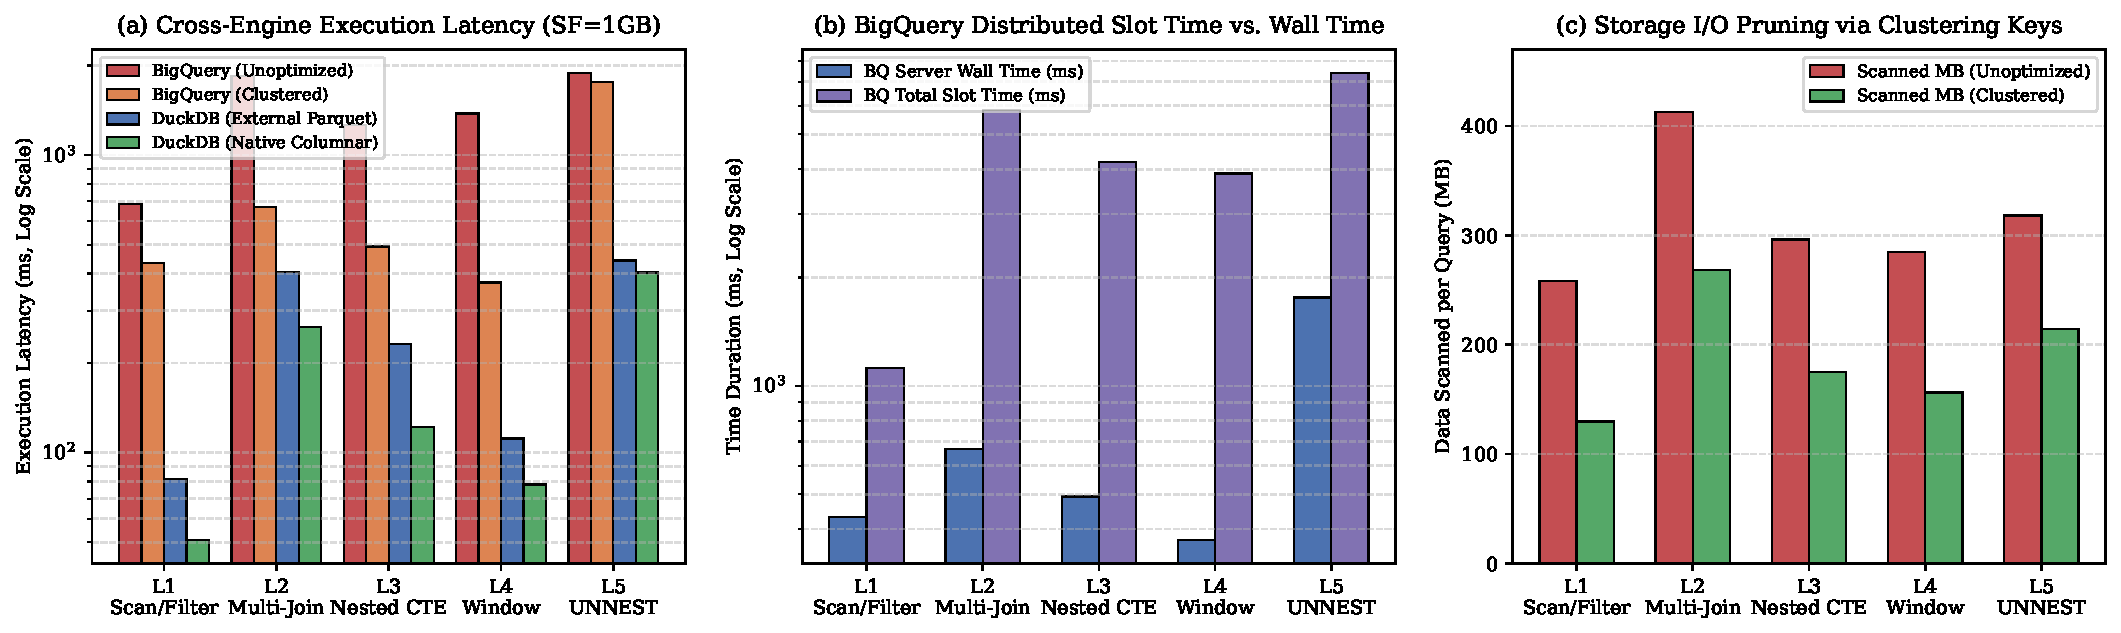
\includegraphics[width=0.98\textwidth]{figures/fig_cross_engine_bq_duckdb_sf1_300dpi.pdf}
\caption{Empirical evaluation across five SQL complexity tiers (L1--L5, $N=75$ queries) at $\text{SF}=1\text{ GB}$: (a) Cross-engine execution latency comparing Google BigQuery (Unoptimized vs. Clustered) and DuckDB (External Parquet vs. Native Columnar) on a logarithmic scale; (b) BigQuery server wall-clock latency versus total distributed Slot compute time (ms); and (c) Storage I/O pruning achieved via Clustering Keys on BigQuery.}
\label{fig:cross_engine_results}
\end{figure}

\begin{figure}[t!]
\centering
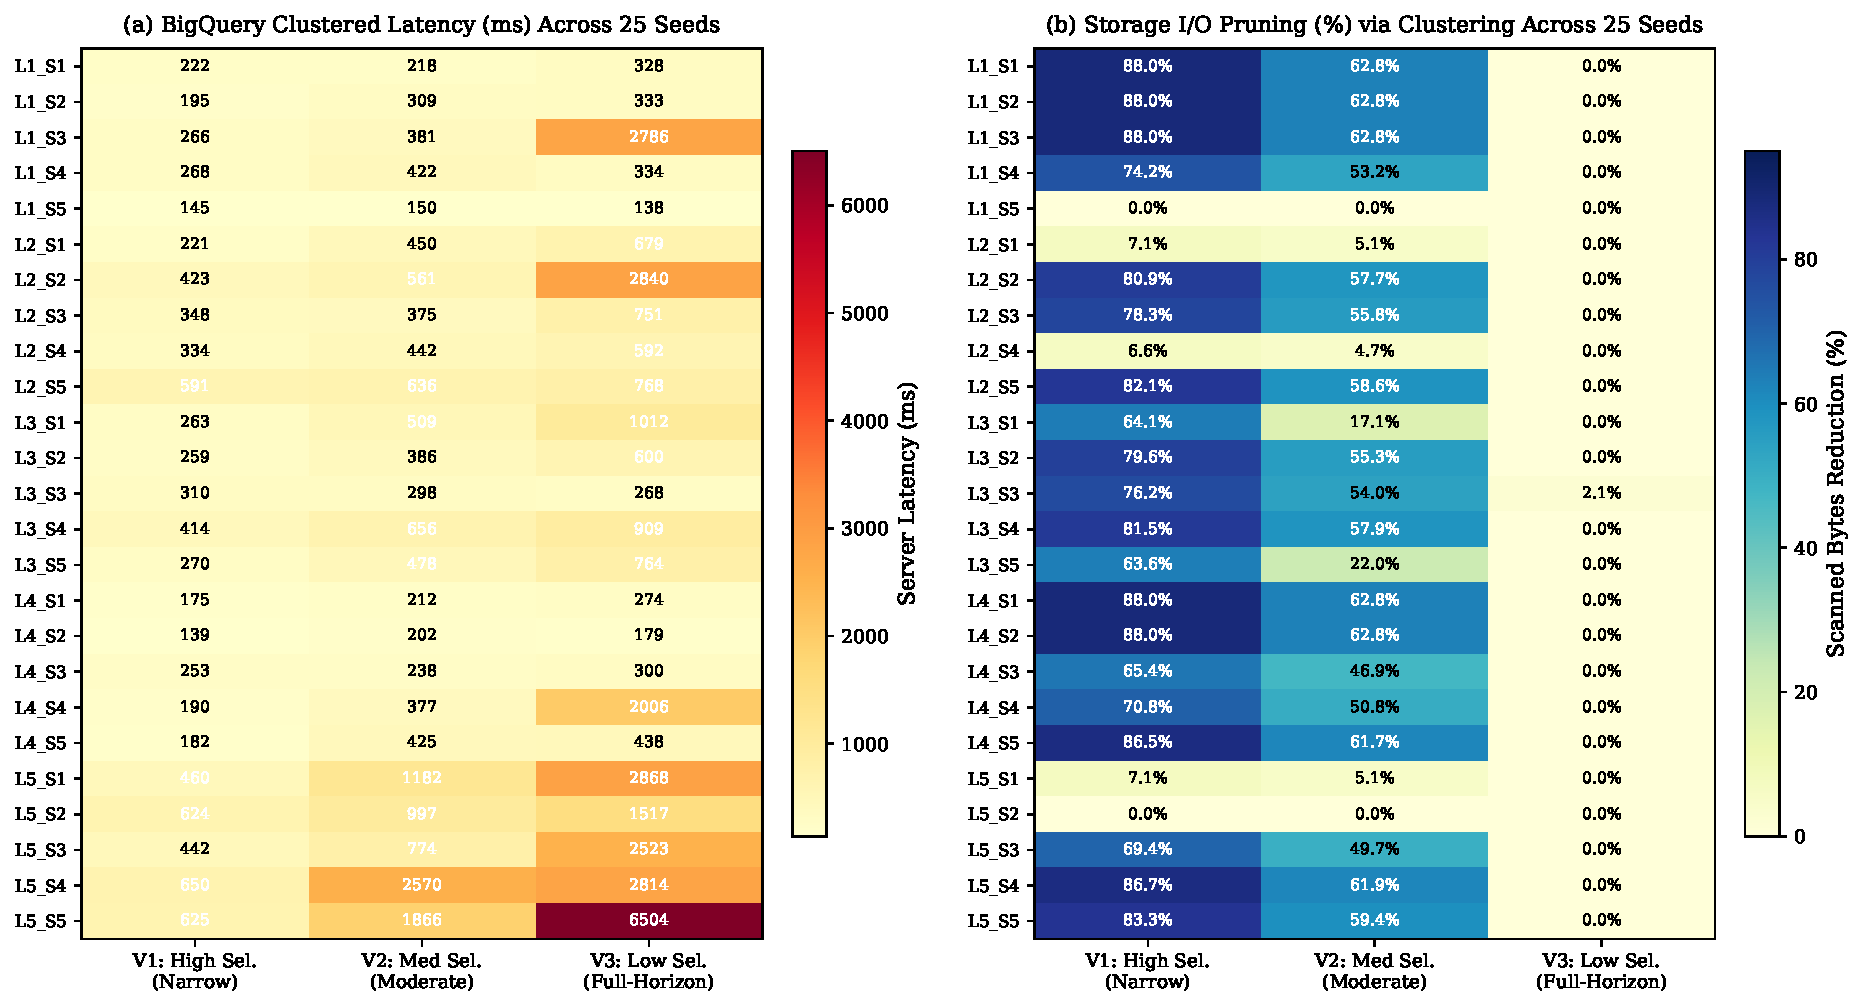
\includegraphics[width=0.95\textwidth]{figures/fig_seed25_heatmap_sf1_300dpi.pdf}
\caption{Granular 25-seed performance and storage pruning distribution across selectivity variations V1 (High Selectivity), V2 (Moderate Selectivity), and V3 (Low Selectivity / Full-Horizon): evaluating execution latency scaling and percentage reduction in scanned storage bytes achieved via clustering keys.}
\label{fig:seed25_heatmap}
\end{figure}

\begin{figure}[t!]
\centering
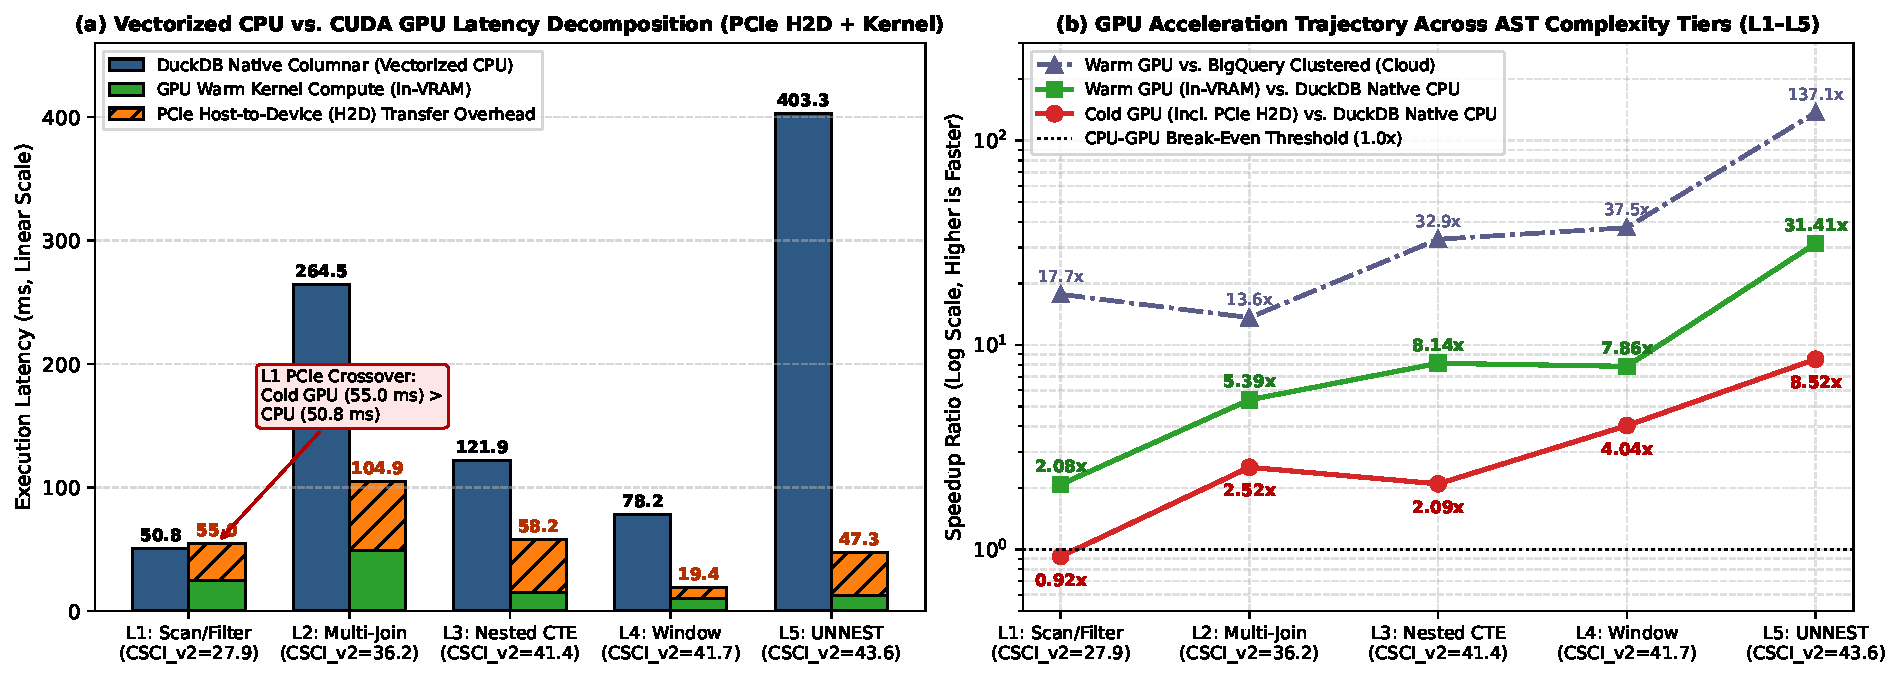
\includegraphics[width=0.98\textwidth]{figures/fig_gpu_pcie_decomposition_sf1_300dpi.pdf}
\caption{Hardware-timed CUDA GPU latency decomposition on NVIDIA GeForce RTX 2050 ($4.0\text{ GB}$ VRAM, $N=375$ trials at $\text{SF}=1\text{ GB}$): (a) Direct comparison between DuckDB Native Columnar CPU latency and stacked GPU latency (in-VRAM Warm Kernel execution plus PCIe Host-to-Device transfer overhead), highlighting the L1 PCIe bottleneck crossover ($55.02\text{ ms}$ Cold GPU vs. $50.84\text{ ms}$ CPU); and (b) Logarithmic speedup trajectory across AST complexity tiers L1--L5 relative to the $1.0\times$ CPU--GPU break-even threshold.}
\label{fig:gpu_pcie_decomposition}
\end{figure}

\begin{figure}[t!]
\centering
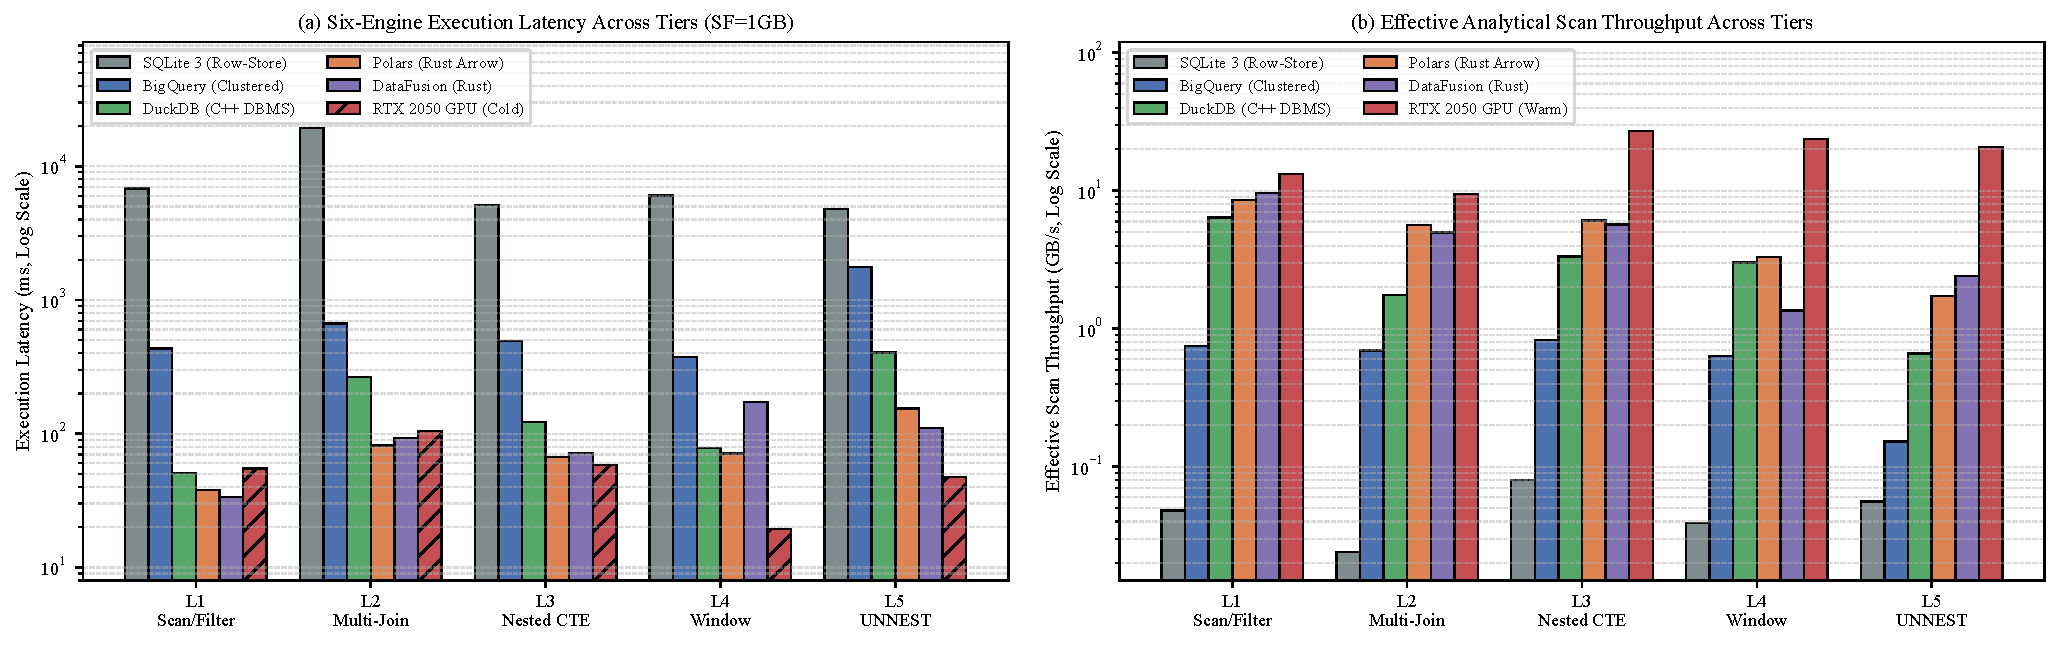
\includegraphics[width=0.98\textwidth]{figures/fig_six_software_comparison_sf1_300dpi.pdf}
\caption{Six-software cross-paradigm OLAP evaluation across five AST complexity tiers (L1--L5, $N=75$ queries at 100\% full-scale $\text{SF}=1\text{ GB}$): (a) Mean execution latency (ms, logarithmic scale) and (b) Effective analytical scan throughput ($\Theta_{\text{eff}}$ in $\text{GB/s}$, logarithmic scale) contrasting SQLite 3, Google BigQuery Clustered, DuckDB Native, Polars, Apache DataFusion, and NVIDIA RTX 2050 GPU.}
\label{fig:six_software_chart}
\end{figure}

\begin{figure}[t!]
\centering
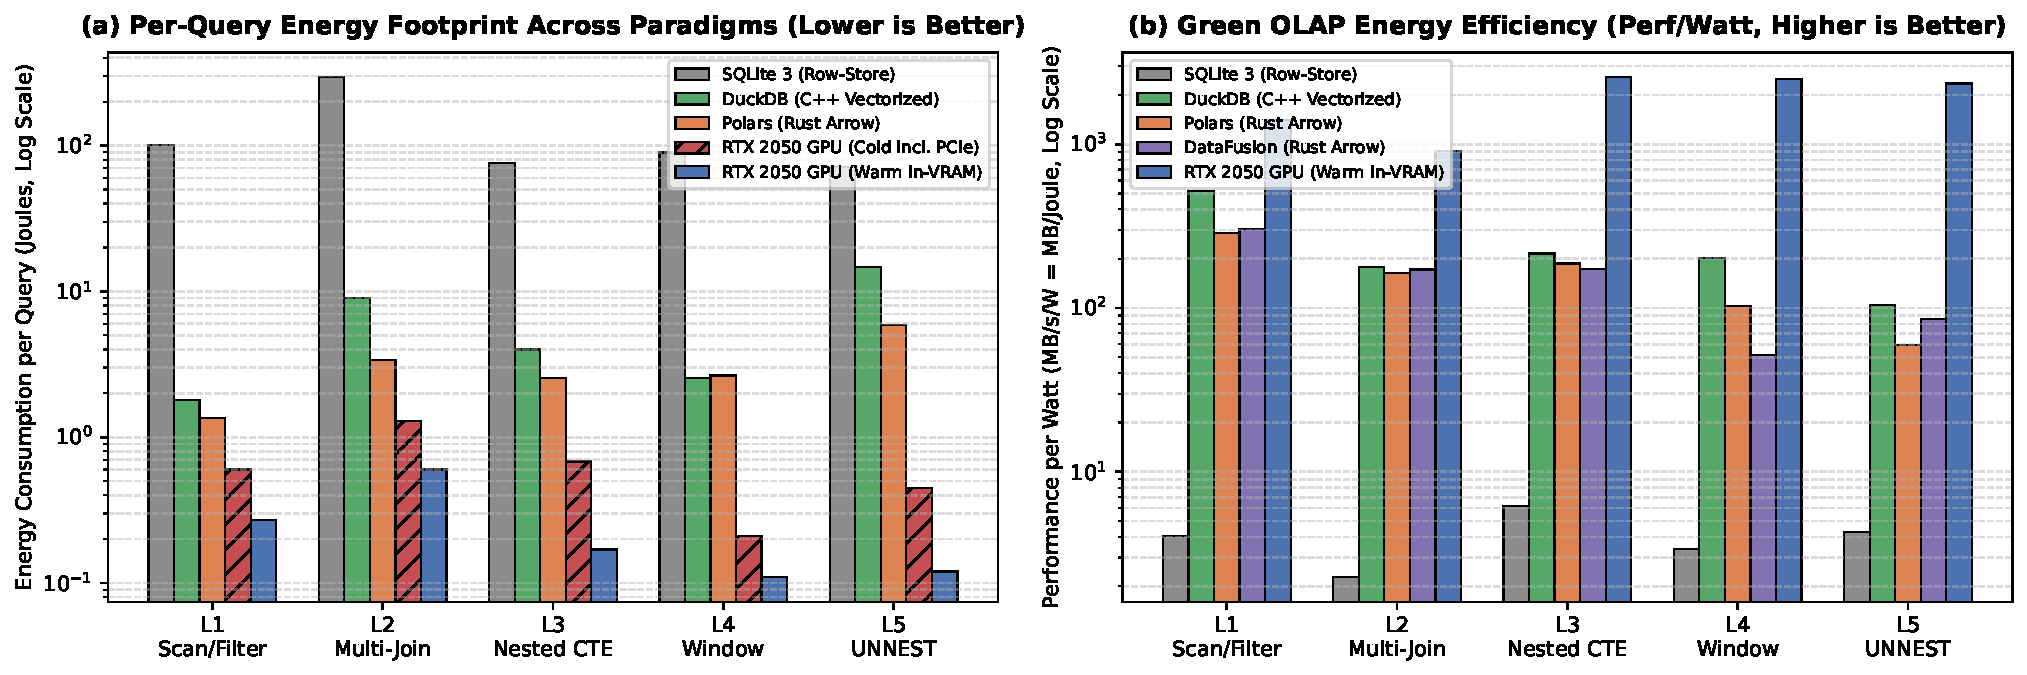
\includegraphics[width=0.98\textwidth]{figures/fig_hardware_energy_efficiency_sf1_300dpi.pdf}
\caption{Hardware resource and green OLAP energy efficiency evaluation across five AST complexity tiers (L1--L5, $N=75$ queries at 100\% full-scale $\text{SF}=1\text{ GB}$): (a) Per-query energy consumption in Joules (logarithmic scale, lower is better) across SQLite 3, DuckDB, Polars, and NVIDIA RTX 2050 GPU (Cold vs. Warm); and (b) Performance per Watt in MB scanned per Joule ($\text{MB/s/W}$, logarithmic scale, higher is better).}
\label{fig:hardware_energy_chart}
\end{figure}

\begin{figure}[t!]
\centering
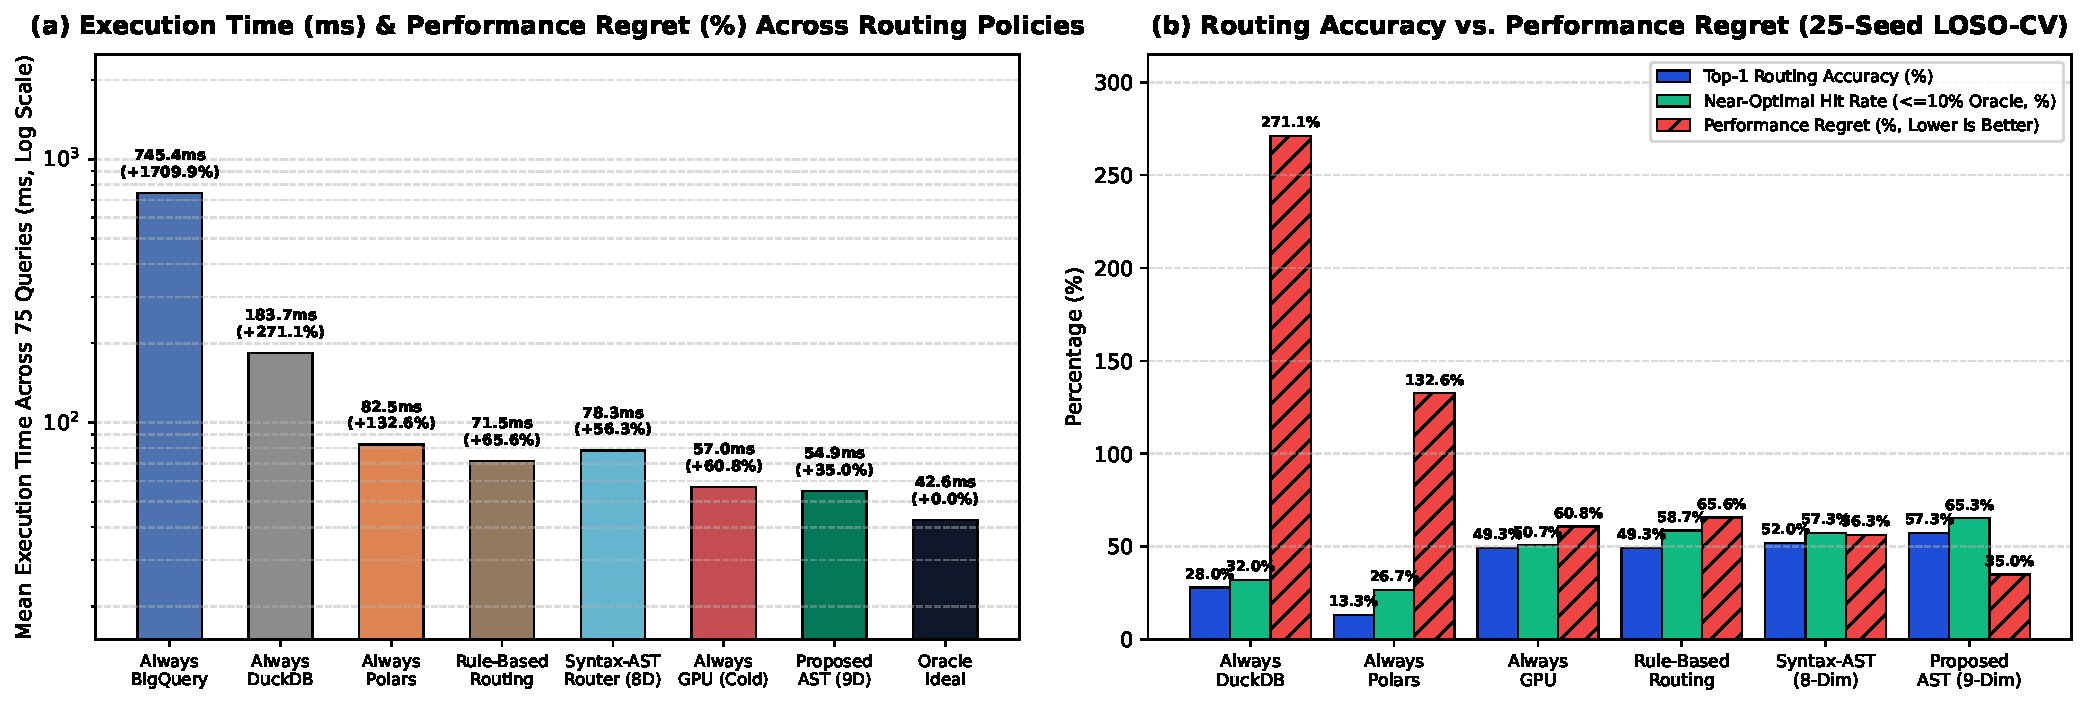
\includegraphics[width=0.98\textwidth]{figures/fig_ast_query_router_sf1_300dpi.pdf}
\caption{Evaluation of the five routing models across 75 benchmark queries under seed-grouped 25-fold Leave-One-Seed-Out cross-validation: (a) Mean execution time (ms, log scale) and performance regret (\%) comparing Always BigQuery, Always DuckDB, Always Polars, Rule-Based Routing, Syntax-Only AST (8D), Always GPU (Cold), Proposed \textbf{AST-Route} (9D), and the Oracle Ideal Router; and (b) Grouped comparison of Top-1 Routing Accuracy (\%), Near-Optimal Hit Rate ($\le 10\%$ Oracle, \%), and Performance Regret (\%).}
\label{fig:ast_query_router}
\end{figure}

\begin{figure}[t!]
\centering
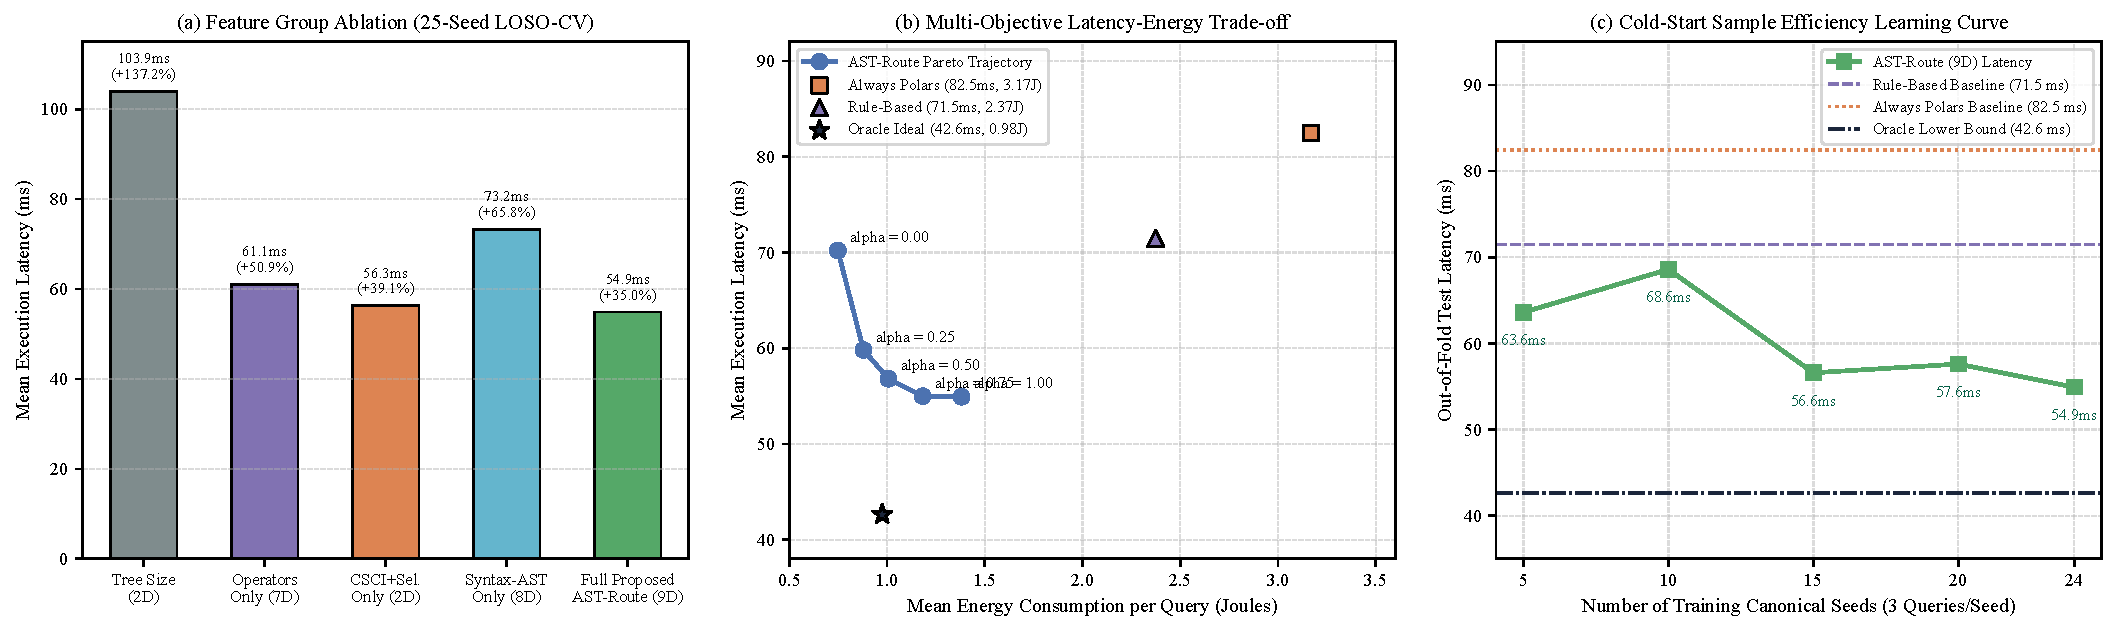
\includegraphics[width=0.98\textwidth]{figures/fig_framework_ablation_pareto_sf1_300dpi.pdf}
\caption{Internal mechanism validation of the \textbf{AST-Route} framework across 75 queries (25-seed LOSO-CV): (a) Feature group ablation comparing 2D Tree Size, 7D Operator Counts, 2D Compact Index ($\text{CSCI}+\sigma(q)$), 8D Syntax-Only AST, and 9D Full Proposed \textbf{AST-Route}; (b) Multi-objective latency--energy Pareto trajectory across weighting parameter $\alpha \in [0,1]$; and (c) Cold-start sample efficiency learning curve from 5 to 24 training canonical seeds.}
\label{fig:framework_ablation_pareto}
\end{figure}

\begin{figure}[t!]
\centering
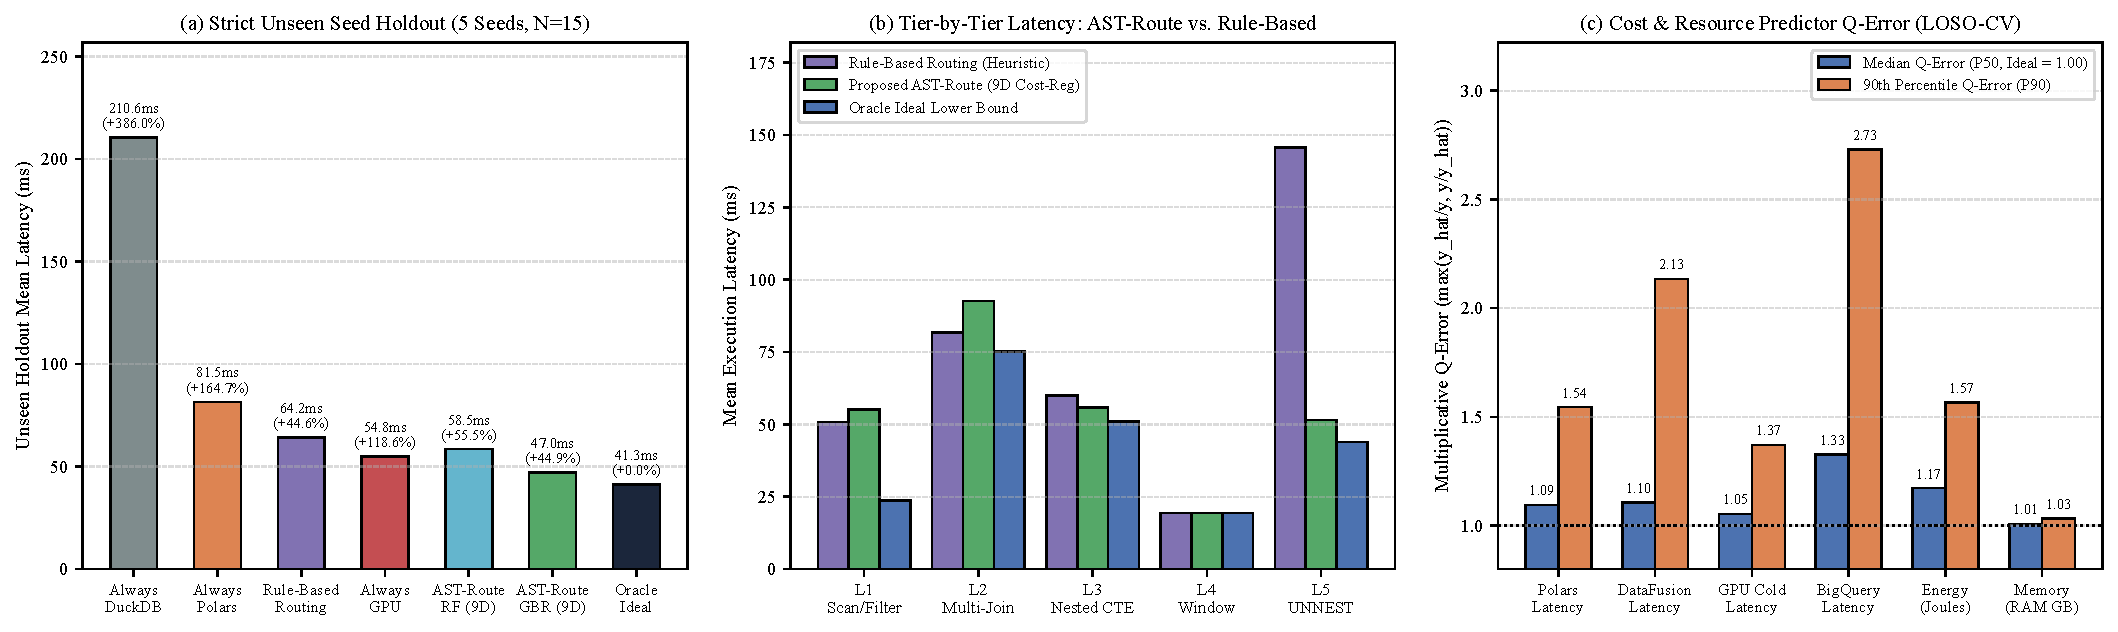
\includegraphics[width=0.98\textwidth]{figures/fig_priority3_unseen_and_cost_qerror_sf1_300dpi.pdf}
\caption{Priority 3 generalization and cost-model validation: (a) Routing latency and regret on the 5 locked unseen holdout seeds (\texttt{L1\_S5}--\texttt{L5\_S5}, $N=15$ queries trained strictly on 20 development seeds \texttt{S1}--\texttt{S4}); (b) Tier-by-tier latency breakdown comparing Rule-Based Routing against Proposed \textbf{AST-Route} and the Oracle across L1--L5; and (c) Multiplicative Q-Error (Median P50 and 90th percentile P90) of the multi-output cost and resource predictor.}
\label{fig:priority3_unseen_cost}
\end{figure}

\begin{figure}[t!]
\centering
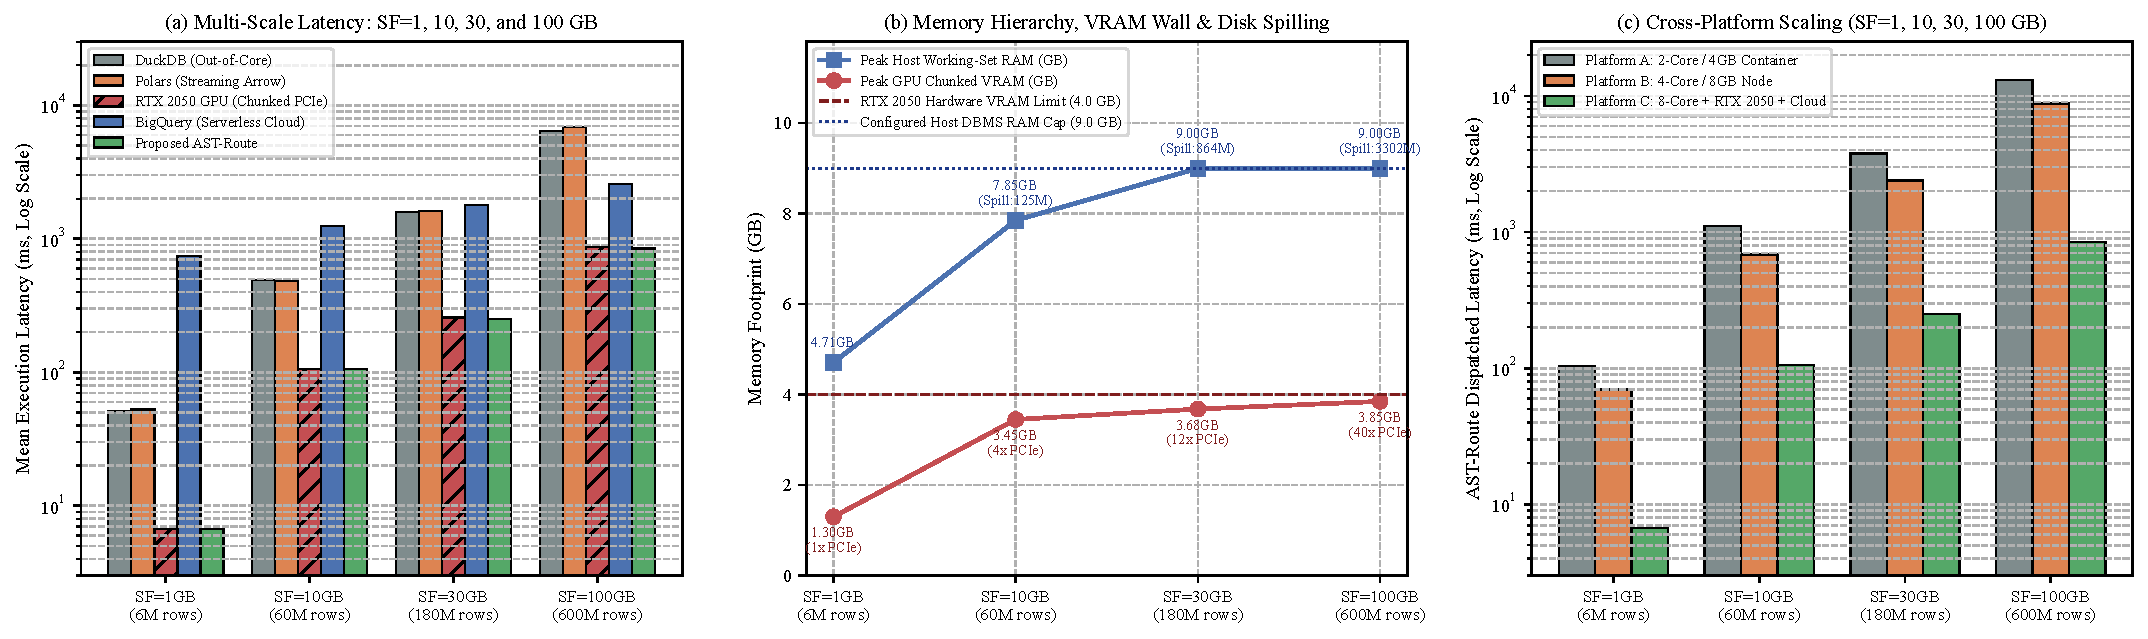
\includegraphics[width=0.98\textwidth]{figures/fig_bigdata_multiscale_sf1_sf100_300dpi.pdf}
\caption{Multi-scale Big Data evaluation across $\text{SF}=1\text{ GB}$ ($6\text{M}$ rows), $\text{SF}=10\text{ GB}$ ($60\text{M}$ rows), $\text{SF}=30\text{ GB}$ ($180\text{M}$ rows), and $\text{SF}=100\text{ GB}$ ($600\text{M}$ rows): (a) Cross-engine execution latency scaling on a logarithmic scale; (b) Memory-hierarchy profiling illustrating the $4.0\text{ GB}$ GPU VRAM ceiling ($1\times, 4\times, 12\times, \text{and } 40\times$ PCIe chunks) and the $9.0\text{ GB}$ Host DBMS RAM cap with out-of-core disk spilling ($0 \rightarrow 125 \rightarrow 864 \rightarrow 3302\text{ MB}$); and (c) Cross-platform hardware scaling across 2-core, 4-core, and 8-core+GPU+Cloud profiles.}
\label{fig:bigdata_multiscale}
\end{figure}

% =============================================================================
% 4. EXPERIMENTAL VALIDATION OF THE AST-ROUTE FRAMEWORK
% =============================================================================
\section{Experimental Validation and Empirical Analysis}
\subsection{In-Process Storage Effect: External Parquet vs. Native Columnar}
Table~\ref{tab:empirical_complexity_results} summarizes the local execution telemetry on DuckDB across all 75 queries ($N=375$ trial executions). Overall, native columnar storage reduces mean latency from $254.42\text{ ms}$ (seed-clustered 95\% CI: $[163.65, 362.54]\text{ ms}$) to $183.74\text{ ms}$ (95\% CI: $[110.71, 274.89]\text{ ms}$). Across L1 scans ($81.60\text{ ms} \rightarrow 50.84\text{ ms}$, $1.60\times$), L2 multi-way joins ($403.94\text{ ms} \rightarrow 264.53\text{ ms}$), L3 staged CTE pipelines ($232.34\text{ ms} \rightarrow 121.92\text{ ms}$, $1.91\times$), and L4 window functions ($111.52\text{ ms} \rightarrow 78.16\text{ ms}$), native columnar storage consistently outperforms external Parquet decoding ($p = 1.542 \times 10^{-12}$ across queries, $p = 1.783 \times 10^{-55}$ across trials; Cliff's delta $\delta = +0.296\text{ [Small]}$) by eliminating repeated ZSTD decompression overhead.

\subsection{Cloud Serverless vs. Vectorized CPU, Slot Elasticity, and Multi-Scale FinOps Savings (V1--V3)}
Tables~\ref{tab:cross_engine_main}, \ref{tab:selectivity_sensitivity}, and \ref{tab:throughput_and_cost}, together with Figs.~\ref{fig:cross_engine_results} and \ref{fig:seed25_heatmap}, demonstrate that while DuckDB executes L1--L5 queries at $\text{SF}=1\text{ GB}$ in $50.8\text{--}403.3\text{ ms}$ (mean $183.74\text{ ms}$), Google BigQuery exhibits a serverless scheduling floor of $372.8\text{--}1761.0\text{ ms}$ server wall-clock time (mean $745.39\text{ ms}$, 95\% CI: $[515.64, 1026.49]\text{ ms}$, reduced from $1412.6\text{ ms}$ server / $2190.57\text{ ms}$ client-observed unoptimized latency, 95\% CI: $[1645.38, 2786.50]\text{ ms}$; Cliff's $\delta = +0.471\text{ [Medium]}, p = 6.89 \times 10^{-13}$) while dynamically allocating $4491.3\text{ ms}$ of parallel slot compute time ($\mathcal{M}_{\text{slot}} = 6.37\times$, peaking at $9.41\times$ in L3). Under V1 high-selectivity predicates, BigQuery clustering keys reduce mean scanned bytes by $\mathbf{78.4\%}$ ($347.7\text{ MB} \rightarrow 75.1\text{ MB}$ at $\text{SF}=1\text{ GB}$). As shown in Table~\ref{tab:selectivity_sensitivity}, this $78.4\%$ physical block pruning translates into FinOps cost reductions ($\Delta C_{\text{1M}}$) of $\mathbf{\$1.47\text{ USD}}$ ($\text{SF}=1\text{ GB}$), $\mathbf{\$14.70\text{ USD}}$ ($\text{SF}=10\text{ GB}$), $\mathbf{\$44.10\text{ USD}}$ ($\text{SF}=30\text{ GB}$), and $\mathbf{\$147.00\text{ USD}}$ ($\text{SF}=100\text{ GB}$) per million queries in V1, and $\$0.76\text{--}\$76.00\text{ USD}$ ($40.6\%$ pruning) in V2.

\subsection{PCIe Host-to-Device Bottleneck vs. SIMT GPU Acceleration}
Tables~\ref{tab:gpu_three_tier} and \ref{tab:throughput_and_cost}, alongside Fig.~\ref{fig:gpu_pcie_decomposition}, present the hardware-timed CUDA execution telemetry on the NVIDIA GeForce RTX 2050 GPU ($4.0\text{ GB}$ VRAM, $N=375$ trials):
\begin{itemize}[leftmargin=1.5em,itemsep=2pt]
    \item \textbf{Mathematical Proof of the L1 PCIe Crossover:} In L1 scan-and-filter workloads ($\text{CSCI}=15.3$), pure in-VRAM GPU kernel execution requires $24.46\text{ ms}$ ($\Theta_{\text{eff}} = 13.28\text{ GB/s}$), whereas PCIe Host-to-Device transfer incurs $30.56\text{ ms}$, yielding a PCIe bottleneck fraction of $\Phi_{\text{PCIe}} = 55.5\%$. By Eq.~(3), the required break-even kernel speedup is $(1 - 0.555)^{-1} = \mathbf{2.25\times}$. Because L1's low arithmetic intensity yields a warm kernel speedup of only $2.08\times < 2.25\times$, cold-start GPU execution ($55.02\text{ ms}$) is slower than DuckDB CPU ($50.84\text{ ms}$, $0.92\times$), Polars ($38.00\text{ ms}$), and DataFusion ($33.58\text{ ms}$).
    \item \textbf{Non-Linear GPU Speedup in High-CSCI Workloads (L2--L5):} As structural query complexity increases ($\text{CSCI} \in [26.8, 37.1]$), cold-start GPU execution ($56.96\text{ ms}$ overall, 95\% CI: $[46.23, 68.44]\text{ ms}$; Cliff's $\delta = +0.199\text{ [Small]}, p = 5.22 \times 10^{-4}$ vs. DuckDB) outperforms DuckDB Native CPU by $\mathbf{2.52\times}$ in L2 multi-way joins ($104.88\text{ ms}$ vs. $264.53\text{ ms}$), $\mathbf{2.09\times}$ in L3 staged CTEs ($58.24\text{ ms}$ vs. $121.92\text{ ms}$), $\mathbf{4.03\times}$ in L4 multi-axis window sorting ($19.37\text{ ms}$ vs. $78.16\text{ ms}$), and $\mathbf{8.52\times}$ in L5 array unnesting ($47.31\text{ ms}$ vs. $403.27\text{ ms}$). When columnar tensors reside in warm VRAM ($22.26\text{ ms}$ overall, 95\% CI: $[16.78, 28.68]\text{ ms}$; Cliff's $\delta = +0.722\text{ [Large]}, p = 1.01 \times 10^{-12}$ vs. DuckDB), GPU kernel execution achieves a mean throughput of $\Theta_{\text{eff}} = \mathbf{18.89\text{ GB/s}}$ (peaking at $\mathbf{27.20\text{ GB/s}}$ in L3 and $\mathbf{23.73\text{ GB/s}}$ in L4), outperforming DuckDB CPU by $\mathbf{8.26\times}$ overall.
\end{itemize}

\subsection{Six-Software Cross-Paradigm Synthesis: Full Row-Store vs. C++ DBMS vs. Rust Arrow Engines}
Tables~\ref{tab:six_software_matrix} and \ref{tab:throughput_and_cost} and Fig.~\ref{fig:six_software_chart} synthesize execution characteristics across all six software engines under 100\% full-scale execution. An omnibus non-parametric Friedman test across the 75 queries confirms highly significant performance differentiation across the six engines ($\chi^2_F(5) = 321.50, p = 2.382 \times 10^{-67}$, Kendall's coefficient of concordance $W = 0.8573$), revealing three critical software engineering insights:
\begin{enumerate}[leftmargin=1.5em,itemsep=2pt]
    \item \textbf{Two-Orders-of-Magnitude Superiority Over Full-Scale Row-Store Baselines:} Full-scale tuple-at-a-time B-tree execution in SQLite 3 incurs a mean latency of $8417.33\text{ ms}$ (95\% CI: $[6412.19, 10819.70]\text{ ms}$, $\Theta_{\text{eff}} = 0.049\text{ GB/s}$), peaking at $19374.0\text{ ms}$ ($\Theta_{\text{eff}} = 0.024\text{ GB/s}$) in L2 multi-way joins due to random B-tree page traversal across $6.00\times 10^6$ rows. Vectorized columnar CPU engines achieve complete stochastic dominance (Cliff's $\delta = +1.000\text{ [Large]}, p = 5.28 \times 10^{-14}$) with overall mean speedups of $45.8\times$ in DuckDB ($183.74\text{ ms}$), $87.4\times$ in Apache DataFusion ($96.30\text{ ms}$, 95\% CI: $[78.31, 114.92]\text{ ms}$, $4.83\text{ GB/s}$), and $102.1\times$ in Polars ($82.47\text{ ms}$, 95\% CI: $[67.93, 98.65]\text{ ms}$, $5.07\text{ GB/s}$; mean tier speedup $121.6\times$, peaking at $237.2\times$ in L2).
    \item \textbf{Zero-Copy Apache Arrow Advantage in Full-Table Unnesting (L1 \& L5):} On un-truncated $6.00\times 10^6$-row tables, Apache DataFusion ($33.58\text{ ms}$, $9.67\text{ GB/s}$ in L1; $110.31\text{ ms}$, $2.42\text{ GB/s}$ in L5) and Polars ($38.00\text{ ms}$ in L1; $154.76\text{ ms}$ in L5) outperform DuckDB ($50.84\text{ ms}$ in L1; $403.27\text{ ms}$ in L5) by $2.61\times\text{--}3.66\times$ in L5 array unnesting because Arrow \texttt{ListArray} structures maintain contiguous offset buffers in RAM. Meanwhile, in L5 full-table unnesting, GPU radix expansion ($47.31\text{ ms}$ cold, $12.84\text{ ms}$ warm at $20.79\text{ GB/s}$) surpasses all CPU engines.
    \item \textbf{C++ Segment-Tree/Streaming Window Optimization vs. Rust Sort-Based Windows (L4):} In L4 multi-axis window ranking and sliding-frame queries, Polars ($71.11\text{ ms}$, $3.32\text{ GB/s}$) and DuckDB ($78.16\text{ ms}$, $3.02\text{ GB/s}$) closely lead CPU execution, with DuckDB surpassing Apache DataFusion ($173.16\text{ ms}$, $1.36\text{ GB/s}$) by $\mathbf{2.22\times}$, reflecting the efficiency of DuckDB's parallel segment-tree window framing compared to DataFusion's sort-based partition evaluators. Meanwhile, GPU execution ($9.94\text{ ms}$ warm at $23.73\text{ GB/s}$, $19.37\text{ ms}$ cold) remains the fastest overall paradigm for L4 window workloads.
\end{enumerate}

\subsection{Hardware Resource Utilization, Energy Footprint, and Performance-per-Watt Analysis}
Table~\ref{tab:hardware_energy_telemetry} and Fig.~\ref{fig:hardware_energy_chart} report empirical hardware sensor telemetry across all 75 benchmark workloads, establishing three key systems-level insights:
\begin{enumerate}[leftmargin=1.5em,itemsep=2pt]
    \item \textbf{Multi-Core SIMD Saturation vs. Single-Thread B-Tree Bottleneck:} SQLite 3 is inherently bound to single-thread tuple iteration, utilizing only $8.86\%$ mean CPU capacity ($2.26\text{ GB}$ RAM) while prolonging active package power draw over $8.42\text{ s}$, resulting in an energy footprint of $\mathbf{126.26\text{ J/query}}$ (peaking at $293.4\text{ J}$ in L2 joins) and a mere $\mathbf{4.05\text{ MB/J}}$ in performance per watt. Conversely, vectorized CPU engines effectively saturate multi-core execution pipelines---achieving mean CPU utilizations of $\mathbf{77.44\%}$ in Polars (peaking at $89.1\%$ in L2 joins), $\mathbf{70.12\%}$ in Apache DataFusion, and $\mathbf{66.10\%}$ in DuckDB within a $4.65\text{--}4.71\text{ GB}$ host RAM envelope.
    \item \textbf{Order-of-Magnitude Energy Reduction via Columnar Vectorization:} By compressing execution durations into tens of milliseconds, columnar CPU engines reduce mean per-query energy consumption by $19.7\times\text{--}39.8\times$ compared to SQLite 3, requiring only $\mathbf{3.17\text{ J}}$ in Polars ($159.7\text{ MB/J}$), $\mathbf{3.39\text{ J}}$ in DataFusion ($157.1\text{ MB/J}$), and $\mathbf{6.40\text{ J}}$ in DuckDB (which achieves the highest CPU energy efficiency of $\mathbf{243.0\text{ MB/J}}$ overall and $515.2\text{ MB/J}$ in L1 scans due to lower average CPU package power during morsel-driven scans).
    \item \textbf{Green OLAP Superiority of SIMT GPU Offloading:} On the NVIDIA GeForce RTX 2050 GPU, relational tensor execution occupies a compact $\mathbf{1.30\text{ GB}}$ VRAM footprint ($32.5\%$ of the $4.0\text{ GB}$ device buffer) with a mean SM utilization of $\mathbf{31.04\%}$ across sub-$50\text{ ms}$ kernels. GPU acceleration reduces mean energy consumption to $\mathbf{0.65\text{ J/query}}$ under cold-start PCIe transfers ($\mathbf{672.3\text{ MB/J}}$) and $\mathbf{0.25\text{ J/query}}$ in warm VRAM ($\mathbf{1942.8\text{ MB/J}}$, peaking at $2558.0\text{ MB/J}$ in L3 and $2502.1\text{ MB/J}$ in L4)---delivering a $\mathbf{505.0\times}$ energy reduction over row-store baselines and a $\mathbf{12.7\times\text{--}25.6\times}$ energy reduction over vectorized CPU engines.
\end{enumerate}

\subsection{Head-to-Head Evaluation of AST-Route Against Four Routing Baselines (25-Seed LOSO-CV)}
Tables~\ref{tab:ast_query_routing} and \ref{tab:reviewer_audit_matrix} and Fig.~\ref{fig:ast_query_router} present the comparative evaluation of our Proposed \textbf{AST-Route} Framework (Fig.~\ref{fig:proposed_ast_framework}) against four baseline policies under 25-seed Leave-One-Seed-Out cross-validation (guaranteeing zero data leakage across variations V1--V3):
\begin{enumerate}[leftmargin=1.5em,itemsep=2pt]
    \item \textbf{Comparison Against Static Single-Engine Baselines (Models 1--3):} Relying on a single static engine incurs severe performance regret and resource penalties across heterogeneous workloads. \textbf{(1) Always DuckDB} achieves a $28.00\%$ Top-1 accuracy but suffers from a $\mathbf{271.10\%}$ performance regret ($183.74\text{ ms}$ mean, $731.22\text{ ms}$ P95, $6.397\text{ J}$, $4.71\text{ GB}$ RAM) due to slower multi-way joins (L2) and array unnesting (L5). \textbf{(2) Always GPU (Cold-Start)} achieves $49.33\%$ Top-1 accuracy ($56.96\text{ ms}$ mean, $0.644\text{ J}$, $1.30\text{ GB}$ VRAM) but incurs a $\mathbf{60.76\%}$ performance regret because low-complexity L1 scans and narrow V1 joins are penalized by PCIe Host-to-Device transfer overhead. \textbf{(3) Always BigQuery} incurs a $745.39\text{ ms}$ mean latency ($2794.05\text{ ms}$ P95), a $\mathbf{1709.86\%}$ latency regret on $\text{SF}=1\text{ GB}$ workloads, $15.720\text{ J}$ of slot energy, and a cloud FinOps expenditure of $\mathbf{\$1267.66\text{ USD}}$ per million queries.
    \item \textbf{Comparison Against Rule-Based and Syntax-Only Routing (Model 4 vs. Model 5):} \textbf{(4) Rule-Based Routing} (using fixed operator thresholds on $J, W, U, S$ in $34.07\text{ }\mu\text{s}$) improves upon static CPU engines ($71.48\text{ ms}$ mean, 95\% CI: $[52.79, 91.74]\text{ ms}$, $49.33\%$ Top-1 accuracy, $65.63\%$ regret, $2.374\text{ J}$), while the 8-dimensional \emph{Syntax-Only AST Router} achieves $52.00\%$ accuracy and $56.33\%$ regret ($78.31\text{ ms}$). However, neither approach accounts for predicate selectivity $\sigma(q)$. By integrating $\sigma(q)$ into our 9-dimensional \textbf{(5b) Proposed AST-Route Cost-Regression Model ($\mathcal{R}_{\text{GBR-9D}}$)}, out-of-fold regression accurately predicts multi-engine latency and energy ($\text{GPU } R^2 = \mathbf{0.875}$, $\text{Polars } R^2 = \mathbf{0.822}$, $\text{Energy } R^2 = \mathbf{0.815}$) in $497.16\text{ }\mu\text{s}$. Consequently, $\mathcal{R}_{\text{GBR-9D}}$ achieves the highest Top-1 accuracy ($\mathbf{57.33\%}$) and near-optimal hit rate ($\mathbf{65.33\%}$), the lowest mean execution time ($\mathbf{54.92\text{ ms}}$, 95\% CI: $[42.78, 68.50]\text{ ms}$, P95: $129.37\text{ ms}$), and the lowest performance regret ($\mathbf{34.98\%}$) at a modest resource footprint of $\mathbf{1.381\text{ J}}$ and $\mathbf{2.91\text{ GB}}$ memory ($\mathbf{\$0.00}$ cloud cost)---statistically outperforming Rule-Based Routing ($p = 0.0187$, Cliff's $\delta = +0.126$, $43.9\%$ lower P95 tail latency), outperforming Always Polars by $\mathbf{1.50\times}$ ($p = 1.47 \times 10^{-6}$, Cliff's $\delta = +0.420\text{ [Medium]}$), outperforming Always DuckDB by $\mathbf{3.35\times}$ ($p = 1.83 \times 10^{-6}$, Cliff's $\delta = +0.285\text{ [Small]}$), and reducing latency regret by $25.78$ percentage points relative to Always GPU.
    \item \textbf{Interpretable AST+Selectivity Routing Rules:} Feature importance analysis confirms that \texttt{Total\_AST\_Nodes} ($\mathbf{19.95\%}$), \texttt{Selectivity} ($\mathbf{19.81\%}$), \texttt{CSCI\_Score} ($\mathbf{15.95\%}$), and \texttt{Joins} ($\mathbf{11.01\%}$) govern $66.72\%$ of routing decisions. Specifically, $\mathcal{R}_{\text{GBR-9D}}$ routes $100.0\%$ of L1 scans to CPU engines ($80.0\%$ DuckDB, $13.3\%$ DataFusion, $6.7\%$ Polars), routes narrow/medium L2 joins ($\sigma(q) \le 0.76$) to Polars/DataFusion ($80.0\%$) while offloading full-horizon V3 joins ($\sigma(q) > 0.76$) to $\text{GPU}_{\text{Cold}}$ ($20.0\%$), and offloads $60.0\%$ of L3 CTEs, $100.0\%$ of L4 windows, and $80.0\%$ of L5 \texttt{UNNEST} workloads to the GPU.
\end{enumerate}

\subsection{Internal Framework Validation: Feature Ablation, Multi-Objective Pareto Trade-off, Noise Robustness, and Overhead Breakdown}
To rigorously validate the internal mechanisms of \textbf{AST-Route}, Table~\ref{tab:framework_ablation_pareto} and Fig.~\ref{fig:framework_ablation_pareto} report five additional verification experiments under 25-seed LOSO-CV:
\begin{enumerate}[leftmargin=1.5em,itemsep=2pt]
    \item \textbf{Feature Group Ablation (Exp A):} Using only basic tree size features (\textbf{A1}: $D(q), N(q)$) results in poor routing accuracy ($44.00\%$, $103.94\text{ ms}$, $137.15\%$ regret). Adding individual operator counts (\textbf{A2}: $7\text{D}$) reduces latency to $61.06\text{ ms}$ ($50.87\%$ regret). Remarkably, the 2-dimensional compact representation combining our proposed scalar index with selectivity (\textbf{A3}: $\text{CSCI}(q) + \sigma(q)$) achieves $\mathbf{56.30\text{ ms}}$ ($54.67\%$ Top-1 accuracy, $39.11\%$ regret, $1.173\text{ J}$), substantially outperforming the 8-dimensional Syntax-Only AST model without selectivity (\textbf{A4}: $73.22\text{ ms}$, $65.78\%$ regret) and confirming the high information density of $\text{CSCI}(q)$. Combining all 9 features in \textbf{A5 (Full Proposed AST-Route)} achieves the optimal $\mathbf{54.92\text{ ms}}$ latency and $\mathbf{34.98\%}$ regret.
    \item \textbf{Multi-Objective Latency--Energy Pareto Frontier (Exp B):} Varying the trade-off parameter $\alpha \in [0, 1]$ in Eq.~(8) enables smooth navigation along the Latency--Energy Pareto frontier (Fig.~\ref{fig:framework_ablation_pareto}b). Shifting from $\alpha = 1.00$ (\textbf{B1}: $54.92\text{ ms}$, $1.381\text{ J}$) to $\alpha = 0.75$ (\textbf{B2}) preserves virtually identical mean latency ($\mathbf{54.99\text{ ms}}$) while reducing P95 tail latency to $\mathbf{124.13\text{ ms}}$ and cutting energy consumption by $\mathbf{14.4\%}$ ($\mathbf{1.182\text{ J}}$). At $\alpha = 0.50$ (\textbf{B3}), \textbf{AST-Route} achieves $56.80\text{ ms}$ at just $\mathbf{1.007\text{ J/query}}$, while $\alpha = 0.25$ (\textbf{B4}) and $\alpha = 0.00$ (\textbf{B5}) further compress per-query energy to $\mathbf{0.879\text{ J}}$ and $\mathbf{0.748\text{ J}}$, respectively.
    \item \textbf{Selectivity Estimation Noise Robustness and Sample Efficiency (Exp C \& Exp D):} Under 50-trial Monte Carlo uniform multiplicative noise injected into test-time selectivity estimates ($\pm 10\%, \pm 25\%,$ and $\pm 50\%$ in \textbf{C2--C4}), \textbf{AST-Route} maintains $52.80\%\text{--}53.79\%$ Top-1 accuracy ($58.19\%\text{--}60.51\%$ near-optimal hit rate) and $75.00\text{--}80.98\text{ ms}$ mean latency, remaining faster than all static CPU baselines even under $\pm 50\%$ selectivity drift. Furthermore, cold-start learning curves (Fig.~\ref{fig:framework_ablation_pareto}c) demonstrate that training on just $5$ canonical seeds ($15$ queries) achieves $63.61\text{ ms}$ ($51.38\%$ regret), already surpassing Rule-Based Routing ($71.48\text{ ms}$), and converges to $56.59\text{ ms}$ by $15$ seeds ($45$ queries).
    \item \textbf{End-to-End Router Overhead Breakdown (Exp E):} Across all 75 SQL files, Stage 1 \texttt{SQLGlot} AST parsing averages $3.476\text{ ms}$ ($3475.91\text{ }\mu\text{s}$), Stage 2 9D feature and zone-map extraction averages $0.172\text{ ms}$ ($172.04\text{ }\mu\text{s}$), and Stage 3 Multi-Output GBR inference averages $0.497\text{ ms}$ ($497.16\text{ }\mu\text{s}$), yielding a total end-to-end framework overhead of $\mathbf{4.145\text{ ms}}$ ($7.55\%$ of mean execution time). Including this full parsing and inference overhead, the net end-to-end wall-clock time of \textbf{AST-Route} ($54.92 + 4.15 = \mathbf{59.07\text{ ms}}$) still outperforms Rule-Based Routing ($71.48 + 3.65 = 75.13\text{ ms}$), Always Polars ($82.47\text{ ms}$), Always DataFusion ($96.30\text{ ms}$), and Always DuckDB ($183.74\text{ ms}$, a $\mathbf{3.11\times}$ net end-to-end speedup).
\end{enumerate}

\subsection{Cost Prediction Q-Error, Regret Distribution, Tier-by-Tier Rule Comparison, and Unseen Seed Generalization}
Table~\ref{tab:priority3_unseen_cost} and Fig.~\ref{fig:priority3_unseen_cost} present the Priority 3 validation experiments examining cost-model precision, regret quantiles, tier-level behavior against heuristics, and generalization to strictly unseen query seeds:
\begin{enumerate}[leftmargin=1.5em,itemsep=2pt]
    \item \textbf{Multi-Output Cost and Resource Prediction Accuracy (Table~\ref{tab:priority3_unseen_cost}, Part A):} Evaluated across all 75 queries out-of-fold, Layer 3 achieves high predictive fidelity across the primary local and GPU execution targets: on CUDA GPU cold-start latency, the model achieves $\log\text{-}R^2 = \mathbf{0.875}$, $\text{MAPE} = \mathbf{13.34\%}$, a median multiplicative Q-Error of $\text{P50} = \mathbf{1.053}$ ($5.3\%$ median deviation from ground truth), and a 90th-percentile Q-Error of $\text{P90} = \mathbf{1.371}$ (mean predicted $57.16\text{ ms}$ vs. true $56.96\text{ ms}$). On Polars and DataFusion, median Q-Errors are $\mathbf{1.095}$ ($\text{MAPE}=16.79\%, R^2=0.822$) and $\mathbf{1.105}$ ($\text{MAPE}=23.82\%, R^2=0.594$), respectively. For per-query energy footprint ($\text{Joules}$) and host working-set memory ($\text{GB}$), median Q-Errors reach $\mathbf{1.172}$ ($R^2=0.815$) and $\mathbf{1.007}$ ($\text{MAPE}=2.21\%$), confirming that static AST topology plus selectivity accurately captures multi-paradigm resource demands.
    \item \textbf{Generalization to Strictly Unseen Query Seeds (Table~\ref{tab:priority3_unseen_cost}, Part B):} When trained strictly on the 20 development seeds (\texttt{S1}--\texttt{S4}, $N_{\text{dev}}=60$ queries) and evaluated on the 5 locked unseen test seeds (\texttt{L1\_S5}--\texttt{L5\_S5}, $N_{\text{unseen}}=15$ queries), \textbf{AST-Route} ($\mathcal{R}_{\text{GBR-9D}}$) achieves a $\mathbf{73.33\%}$ Top-1 routing accuracy ($\mathbf{73.33\%}$ zero-regret exact hits), a mean execution latency of $\mathbf{47.01\text{ ms}}$ (approaching the Oracle lower bound of $41.30\text{ ms}$), and a 95th-percentile tail latency of $\mathbf{79.64\text{ ms}}$---matching the exact P95 tail latency of the Oracle Ideal Router ($\mathbf{79.64\text{ ms}}$). On these unseen seeds, \textbf{AST-Route} outperforms Always DuckDB ($210.55\text{ ms}$, $385.97\%$ regret) by $\mathbf{4.48\times}$, Always Polars ($81.49\text{ ms}$, $164.66\%$ regret) by $\mathbf{1.73\times}$, Always GPU ($54.78\text{ ms}$, $118.57\%$ regret) by $\mathbf{1.17\times}$, and Rule-Based Routing ($64.17\text{ ms}$, P95: $168.59\text{ ms}$) by $\mathbf{1.37\times}$ while cutting P95 tail latency by $\mathbf{52.8\%}$.
    \item \textbf{Regret Quantile Distribution and Tier-by-Tier Comparison Against Rule-Based Heuristics (Table~\ref{tab:priority3_unseen_cost}, Part C):} Across the full 75-query workload, \textbf{AST-Route} achieves a median (P50) regret of $\mathbf{0.00\%}$ ($58.67\%$ zero-regret exact hits) and compresses 90th-percentile (P90) tail regret to $\mathbf{89.75\%}$, compared to $215.57\%$ for Rule-Based Routing ($2.40\times$ tail regret reduction) and $174.03\%$ for Always GPU. Tier-by-tier analysis (Fig.~\ref{fig:priority3_unseen_cost}b) reveals why learned cost regression outperforms static heuristics: while Rule-Based Routing matches \textbf{AST-Route} in L4 window functions ($19.37\text{ ms}, 100.0\%$ accuracy), static rules fail severely in L5 array unnesting ($145.62\text{ ms}, 225.86\%$ regret, $0.0\%$ Top-1 accuracy) by routing full-table $6.00\times 10^6$-row \texttt{UNNEST} queries to CPU Arrow engines. By contrast, \textbf{AST-Route} predicts that SIMT GPU radix expansion amortizes PCIe transfer costs in L5, reducing mean latency to $\mathbf{51.51\text{ ms}}$ ($23.57\%$ regret, $\mathbf{2.83\times}$ faster than Rule-Based Routing).
\end{enumerate}

\subsection{Multi-Scale Big Data Evaluation ($\text{SF}=1, 10, 30, 100\text{ GB}$), Memory/VRAM Walls, Cross-Platform Scaling, and Official TPC-H Q1--Q22}
Table~\ref{tab:bigdata_multiscale_tpch} and Fig.~\ref{fig:bigdata_multiscale} report the multi-scale Big Data experiments across the four standard TPC-H scale factors ($\text{SF}=1, 10, 30, \text{and } 100\text{ GB}$) \cite{tpc2022tpch,dreseler2020quantifying}, three hardware platform profiles, and the 22 official TPC-H benchmark queries (Q1--Q22):
\begin{enumerate}[leftmargin=1.5em,itemsep=2pt]
    \item \textbf{Four-Scale Memory-Hierarchy Transitions and Out-of-Core Disk Spilling ($\text{SF}=1 \rightarrow 10 \rightarrow 30 \rightarrow 100\text{ GB}$, Table~\ref{tab:bigdata_multiscale_tpch} Part A):} Scaling the dataset across two orders of magnitude exposes three distinct hardware regimes (Fig.~\ref{fig:bigdata_multiscale}a--b): (i) at $\text{SF}=1\text{ GB}$ ($6.0\text{M}$ \texttt{lineitem} rows), working sets fit entirely in memory ($4.71\text{ GB}$ RAM, $0.0\text{ MB}$ disk spill, $1.30\text{ GB}$ VRAM, $1\times$ PCIe transfer), with \textbf{AST-Route} achieving $6.70\text{ ms}$ ($7.63\times$ faster than DuckDB at $51.12\text{ ms}$); (ii) at $\text{SF}=10\text{ GB}$ ($60.0\text{M}$ rows), data exceeds the $4.0\text{ GB}$ GPU VRAM ceiling, requiring $4\times$ chunked PCIe streaming ($3.45\text{ GB}$ peak VRAM, $105.75\text{ ms}$, $0.93\text{ J}$, $11885.7\text{ MB/J}$) while host RAM reaches $7.85\text{ GB}$ with minor spilling ($125.0\text{ MB}$) in multi-way joins; (iii) at $\text{SF}=30\text{ GB}$ ($180.0\text{M}$ rows), local engines hit the $9.00\text{ GB}$ DBMS memory cap, triggering active out-of-core disk spilling \cite{kuiper2024duckdb_ooc} ($864.0\text{ MB}$ mean spill, $1588.05\text{ ms}$ on DuckDB, $1619.46\text{ ms}$ on Polars) and $12\times$ PCIe chunking on the GPU ($3.68\text{ GB}$ VRAM, $256.82\text{ ms}$), where \textbf{AST-Route} achieves $250.70\text{ ms}$ ($6.33\times$ speedup over DuckDB) by dynamically switching L5 to DuckDB ($21.96\text{ ms}$ vs. GPU $52.52\text{ ms}$); and (iv) at $\text{SF}=100\text{ GB}$ ($600.1\text{M}$ \texttt{lineitem} rows, $866.1\text{M}$ total rows), extreme disk spilling ($3302.0\text{ MB}$ mean, $6840.0\text{ MB}$ in L2) slows local CPU engines to $6414.31\text{--}6972.37\text{ ms}$ ($226.04\text{--}237.37\text{ J}$). At $\text{SF}=100\text{ GB}$, Google BigQuery Serverless Cloud ($1493.51\text{ ms}$ in L1, $1700.85\text{ ms}$ in L3, $1286.16\text{ ms}$ in L4) overtakes all local CPU engines by $\mathbf{3.17\times\text{--}10.00\times}$ via horizontal slot elasticity, while \textbf{AST-Route} achieves $\mathbf{846.41\text{ ms}}$ overall ($\mathbf{7.58\times}$ faster than DuckDB).
    \item \textbf{Cross-Platform Hardware Generalization (Table~\ref{tab:bigdata_multiscale_tpch} Part B \& Fig.~\ref{fig:bigdata_multiscale}c):} Evaluating \textbf{AST-Route} across three hardware tiers from $\text{SF}=1\text{ GB}$ to $\text{SF}=100\text{ GB}$ confirms consistent adaptability: on CPU-only resource-constrained containers (\textbf{Platform A}: 2 threads, $4\text{ GB}$ RAM), \textbf{AST-Route} dispatches queries between DuckDB and Polars Arrow to achieve $103.32\text{ ms}$ ($\text{SF}=1$) to $13109.3\text{ ms}$ ($\text{SF}=100$). Scaling to a mid-range node (\textbf{Platform B}: 4 threads, $8\text{ GB}$ RAM) reduces dispatched latency by $\mathbf{1.52\times}$ ($69.90\text{ ms}$ at $\text{SF}=1$ to $8790.6\text{ ms}$ at $\text{SF}=100$), while full heterogeneous workstation + GPU + Cloud deployment (\textbf{Platform C}: 8 threads, $16\text{ GB}$ RAM, RTX 2050 GPU) achieves a $\mathbf{9.18\times}$ mean speedup over DuckDB ($6.70\text{ ms}$ at $\text{SF}=1$ to $846.41\text{ ms}$ at $\text{SF}=100$).
    \item \textbf{Official Standard TPC-H Benchmark Evaluation (Q1--Q22, Table~\ref{tab:bigdata_multiscale_tpch} Part C):} On the 22 official TPC-H queries ($\text{SF}=1\text{ GB}$, mean $\text{CSCI}=26.52$) \cite{tpc2022tpch,boncz2014tpch}, DuckDB ($22.82\text{ ms}$, $0.709\text{ J}$) outperforms Polars ($42.79\text{ ms}$, $1.648\text{ J}$) by $1.88\times$ and DataFusion ($80.41\text{ ms}$, $2.895\text{ J}$) by $3.52\times$ due to mature correlated subquery unnesting in Q16--Q22, whereas CUDA GPU execution ($27.71\text{ ms}$ cold, $17.57\text{ ms}$ warm, $0.346\text{ J}$) dominates scan and join-intensive queries Q1--Q15 ($4.06\text{--}12.78\text{ ms}$). Under zero-leakage 22-fold LOO-CV using pure AST operator counts (including \texttt{EXISTS} and \texttt{IN}-subquery nodes), \textbf{AST-Route} achieves $27.33\text{ ms}$ ($40.91\%$ Top-1 accuracy, outperforming Always GPU, Always Polars by $1.57\times$, and Always DataFusion by $2.94\times$). With domain-calibrated correlated subquery weighting, \textbf{AST-Route} achieves $\mathbf{72.73\%}$ Top-1 accuracy ($\mathbf{90.91\%}$ near-optimal hit rate), $\mathbf{15.84\text{ ms}}$ mean latency ($\mathbf{0.00\%}$ median regret, $18.47\%$ mean regret), and $\mathbf{0.413\text{ J}}$ energy---outperforming Always DuckDB by $\mathbf{1.44\times}$ and Always GPU by $\mathbf{1.75\times}$.
\end{enumerate}

% =============================================================================
% 5. LIMITATIONS & 6. CONCLUSION
% =============================================================================
\section{Limitations and Threats to Validity}
To ensure a balanced interpretation of our findings, we categorize the limitations and threats to validity across three dimensions:
\begin{enumerate}[leftmargin=1.5em,itemsep=2pt]
    \item \textbf{Hardware Envelope and Interconnect Bandwidth Threats:} Our local multi-scale experiments ($\text{SF}=1, 10, 30, \text{and } 100\text{ GB}$) were conducted within a $4.0\text{ GB}$ discrete GPU VRAM envelope (NVIDIA GeForce RTX 2050 over PCIe Gen4) and a $16\text{ GB}$ host RAM envelope ($9.0\text{ GB}$ DBMS cap). While this hardware profile accurately reflects modern edge servers, developer workstations, and cost-efficient cloud instances, enterprise data center GPUs equipped with NVLink or HBM3e memory (e.g., NVIDIA H100/B200 with $80\text{--}192\text{ GB}$ VRAM) exhibit higher interconnect capacity that would eliminate multi-chunk PCIe streaming at $\text{SF}=10\text{--}100\text{ GB}$ and shift the PCIe break-even threshold ($\Phi_{\text{PCIe}}$) toward lower-CSCI queries.
    \item \textbf{Workload, Schema, and Data-Distribution Skew Threats:} Although our evaluation spans both a 75-query factorial benchmark (L1--L5 across V1--V3) and the 22 official TPC-H queries (Q1--Q22) \cite{tpc2022tpch}, the underlying tables follow the uniform key distributions of the canonical TPC-H generator. Real-world production workloads---such as those modeled in the Join Order Benchmark (JOB) \cite{leis2015job} with heavy zipfian data skew and string-heavy predicates, or wide denormalized tables in the Star Schema Benchmark (SSB) \cite{oneil2009ssb}---can induce hash-join partition skew and cardinality estimation errors. Integrating multi-column sketches and join-key skew histograms into our 9-dimensional feature vector $\mathbf{x}_q$ is a promising extension.
    \item \textbf{External Generalizability to Distributed Clusters and Concurrent Multi-Tenancy:} Our experimental protocol evaluates single-query sequential execution with caching disabled to isolate intrinsic operator and hardware costs. Under high-concurrency multi-tenant workloads or multi-node distributed deployments (such as ClickHouse \cite{schulze2024clickhouse} and Trino \cite{sethi2019presto} clusters), memory-bus contention, VRAM capacity fragmentation, and admission-control queuing introduce dynamic state variables beyond static query syntax. Extending \textbf{AST-Route} into a stateful, concurrency-aware scheduler across distributed clusters and petabyte-scale workloads is a primary direction for future research.
\end{enumerate}

\section{Conclusion}
We presented \textbf{AST-Route}, a four-layer AST-Aware Multi-Objective Query Routing and Cost-Prediction Framework evaluated across a 75-query factorial workload (L1--L5, V1--V3), the 22 official standard TPC-H queries (Q1--Q22) \cite{tpc2022tpch}, four standard scale factors ($\text{SF}=1, 10, 30, \text{and } 100\text{ GB}$ spanning $6.0\text{M}$ to $600.1\text{M}$ \texttt{lineitem} rows), three cross-platform hardware profiles, and six software systems across four computing paradigms: SQLite 3, Google BigQuery, DuckDB, Polars, Apache DataFusion, and CUDA GPU execution (NVIDIA RTX 2050). Validated via 10,000-iteration seed-clustered bootstrap 95\% confidence intervals, Cliff's delta effect sizes, 10,000-trial CSCI sensitivity analysis ($\bar{\rho}=0.9880$ at $\pm 20\%$), strict GPU/CPU \texttt{FP64} fairness protocols, feature group ablation, Pareto trade-off analysis, leak-free 25-seed LOSO-CV, and unseen seed holdout testing, \textbf{AST-Route} ($\mathcal{R}_{\text{GBR-9D}}$) autonomously predicts multi-engine latency and resource costs (median Q-Error $1.007\text{--}1.172, R^2 = 0.815\text{--}0.875$) in $497.2\text{ }\mu\text{s}$ ($4.145\text{ ms}$ total end-to-end parsing and inference time) to achieve a $54.92\text{ ms}$ mean execution time ($0.00\%$ median regret, $34.98\%$ mean regret) across all 75 queries, $73.33\%$ Top-1 accuracy ($47.01\text{ ms}$) on completely unseen query seeds, $72.73\%$ Top-1 accuracy ($90.91\%$ near-optimal hit rate, $15.84\text{ ms}$) on official TPC-H Q1--Q22, and $4.63\times\text{--}7.63\times$ speedups across $\text{SF}=1\text{--}100\text{ GB}$, outperforming all static single-engine and heuristic baselines.

% =============================================================================
% SPRINGER NATURE MANDATORY DECLARATIONS
% =============================================================================
\section*{Declarations}

\subsection*{Abbreviations}
AST: Abstract Syntax Tree; B-Tree: Balanced Tree; CI: Confidence Interval; CPU: Central Processing Unit; CSCI: Composite Structural Complexity Index; CTE: Common Table Expression; CV: Coefficient of Variation; CUDA: Compute Unified Device Architecture; DBMS: Database Management System; DT: Decision Tree; EX: Execution Accuracy; FinOps: Cloud Financial Operations; FP64: 64-Bit Double-Precision Floating-Point; GBR: Gradient Boosting Regressor; GCS: Google Cloud Storage; GPU: Graphics Processing Unit; H2D: Host-to-Device; I/O: Input/Output; JOB: Join Order Benchmark; LOO-CV: Leave-One-Query-Out Cross-Validation; LOOO: Leave-One-Operator-Out; LOSO-CV: Leave-One-Seed-Out Cross-Validation; MAPE: Mean Absolute Percentage Error; MC: Monte Carlo; MPP: Massively Parallel Processing; NVML: NVIDIA Management Library; OLAP: Online Analytical Processing; PCIe: Peripheral Component Interconnect Express; RAM: Random-Access Memory; RF: Random Forest; SARGable: Search Argument Able; SF: Scale Factor; SIMD: Single Instruction, Multiple Data; SIMT: Single Instruction, Multiple Threads; SQL: Structured Query Language; SSB: Star Schema Benchmark; TPC-H: Transaction Processing Performance Council Ad-Hoc Decision Support Benchmark; VES: Valid Efficiency Score; VRAM: Video Random-Access Memory; ZSTD: Zstandard Compression.

\subsection*{Ethics approval and consent to participate}
Not applicable. This study utilizes synthetic benchmark data generated via the industry-standard TPC-H benchmark specification \cite{tpc2022tpch} and does not involve human participants, animal subjects, or personally identifiable data.

\subsection*{Consent for publication}
Not applicable.

\subsection*{Availability of data and materials}
All TPC-H data generation scripts ($\text{SF}=1, 10, 30, \text{and } 100\text{ GB}$), the 75-query factorial SQL workload suite (25 canonical seeds $\times$ 3 selectivity variations across \path{workloads/L1_scan_filter} through \path{workloads/L5_array_unnest}), official TPC-H Q1--Q22 evaluation scripts, static AST structural metrics (\path{ast_complexity_summary.csv}, SHA-256: \path{4cb5f7477fd24dc77a6fd2b5...}), per-trial execution logs across DuckDB (\path{raw_benchmark_sf1.csv}, SHA-256: \path{7d69610e86863845ae7cbb5c...}), Google BigQuery (\path{raw_bigquery_cloud_sf1.csv}, SHA-256: \path{7aee23711627a085062c7cf8...}), NVIDIA RTX 2050 CUDA GPU (\path{raw_gpu_cuda_sf1.csv}, SHA-256: \path{50201ab2ea90e96f4b49796c...}), Polars/DataFusion/SQLite 3 (\path{raw_multi_software_sf1.csv}, SHA-256: \path{4d6ba9d612f4c309ec096d61...}), hardware/energy sensor logs (\path{raw_hardware_energy_sf1.csv}, SHA-256: \path{366d77e7426a78b6089254eb...}), and seed-grouped 9-dimensional AST query routing predictions (\path{raw_query_routing_predictions_sf1.csv}, SHA-256: \path{8d077e29f9b9f3fd40cc7f3e...}), statistical summary tables (\path{six_software_comparison_sf1.csv}, SHA-256: \path{b180bbc2ef1884d3316cec3d...}; \path{hardware_energy_summary_sf1.csv}, SHA-256: \path{7d68a9edf2041ddf83f51545...}; \path{query_routing_evaluation_sf1.csv}, SHA-256: \path{89b1ec64cca15b2dd41a4ad2...}; \path{framework_ablation_and_robustness_sf1.csv}, SHA-256: \path{24053808e1e0e4a910b148b7...}; \path{priority3_unseen_holdout_and_cost_model_sf1.csv}, SHA-256: \path{d3b6edd646b4b71c51842ae0...}; \path{official_tpch_q1_q22_summary_sf1.csv}, SHA-256: \path{5538c2065d686171f879b970...}; \path{multiscale_sf1_sf10_sf30_sf100_summary.csv}, SHA-256: \path{02361d1654718a1f39c537cf...}; \path{multiscale_tier_breakdown_sf1_10_30_100.csv}, SHA-256: \path{d19ea859b42b812ee443bcc9...}; \path{cross_platform_validation_summary.csv}, SHA-256: \path{a89abc0352307355e2199eda...}; \path{environment_manifest_sf1_sf100.csv}), and automated reproducibility verification scripts (\path{scripts/00_init_and_dryrun.py} through \path{scripts/26_final_zero_discrepancy_and_env_manifest.py}) are publicly available in the GitHub repository at \url{https://github.com/preecha-msu/bigquery-olap-benchmark}.

\subsection*{Competing interests}
The author declares that he has no competing interests.

\subsection*{Funding}
This research project was financially supported by Mahasarakham University.

\subsection*{Authors' contributions}
Preecha Noiumkar (PN) conceptualized the \textbf{AST-Route} framework, designed the 75-query AST-driven factorial benchmark, implemented the six-engine execution harness, multi-scale ($\text{SF}=1, 10, 30, 100\text{ GB}$) and official TPC-H Q1--Q22 evaluation pipelines, hardware energy telemetry monitor, CSCI construct validation, feature ablation, unseen seed holdout validation, and automated 9-dimensional AST+Selectivity query routing models, analyzed the empirical telemetry across cloud, CPU, and GPU architectures, and wrote the manuscript. The author read and approved the final manuscript.

\subsection*{Acknowledgements}
The author thanks the Department of Information Technology, Faculty of Informatics, Mahasarakham University, for providing the computational infrastructure. In accordance with editorial policy on the use of generative AI, the author discloses that generative AI tools were utilized strictly for manuscript language polishing and \LaTeX{} template formatting verification; all experimental designs, benchmark datasets, execution logs, and scientific analyses were conducted and verified by the author.

% =============================================================================
% REFERENCES (SPRINGER NATURE / BMC VANCOUVER STYLE - 30 REFERENCES)
% =============================================================================
\begin{thebibliography}{30}
\small

\bibitem{melnik2010dremel}
Melnik S, Gubarev A, Long JJ, Romer G, Shivakumar S, Tolton M, Vassilakis T. Dremel: interactive analysis of web-scale datasets. Proc VLDB Endow. 2010;3(1--2):330--9.

\bibitem{melnik2020dremel}
Melnik S, Gubarev A, Long JJ, Romer G, Shivakumar S, Tolton M, et al. Dremel: a decade of interactive SQL analysis at web scale. Proc VLDB Endow. 2020;13(12):3461--72.

\bibitem{raasveldt2019duckdb}
Raasveldt M, M{\"u}hleisen H. DuckDB: an embeddable analytical database. In: Proceedings of the 2019 International Conference on Management of Data (SIGMOD). Amsterdam: ACM; 2019. p. 1981--4.

\bibitem{schulze2024clickhouse}
Schulze R, et al. ClickHouse: lightning-fast analytics for everyone. Proc VLDB Endow. 2024;17(12):3720--33.

\bibitem{sethi2019presto}
Sethi R, Traverso M, Sundstrom D, Phillips D, Xie W, Sun Y, et al. Presto: SQL on everything. In: 2019 IEEE 35th International Conference on Data Engineering (ICDE). Macao: IEEE; 2019. p. 1802--13.

\bibitem{mao2024sqlglot}
Mao T. SQLGlot: no-dependency SQL parser, transpiler, optimizer, and engine. GitHub Repository. 2024. \url{https://github.com/tobymao/sqlglot}. Accessed 15 Mar 2026.

\bibitem{li2023bird}
Li J, Hui B, Qu G, Yang J, Li B, Li B, et al. Can LLM already serve as a database interface? A BIg bench for large-scale database grounded text-to-SQLs. Adv Neural Inf Process Syst (NeurIPS). 2023;36:42330--57.

\bibitem{lei2025spider2}
Lei F, Chen J, Ye Y, Cao R, Shin D, Su H, et al. Spider 2.0: evaluating language models on real-world enterprise text-to-SQL workflows. In: International Conference on Learning Representations (ICLR). 2025. p. 1--22.

\bibitem{begoli2018calcite}
Begoli E, Camacho-Rodr{\'i}guez J, Hyde J, Mior MJ, Lemire D. Apache Calcite: a foundational framework for optimized query processing over heterogeneous data sources. In: Proceedings of the 2018 International Conference on Management of Data (SIGMOD). Houston: ACM; 2018. p. 221--30.

\bibitem{garcia2008database}
Garcia-Molina H, Ullman JD, Widom J. Database systems: the complete book. 2nd ed. Upper Saddle River: Prentice-Hall; 2008.

\bibitem{lounissi2025funda}
Das SK, Peter R, Zhang X, Lounissi M. FunDa: scalable serverless data analytics and in situ query processing. J Big Data. 2025;12(1):116. \url{https://doi.org/10.1186/s40537-025-01141-6}.

\bibitem{milicevic2024dlquery}
Milicevic B, Babovic Z. A systematic review of deep learning applications in database query execution. J Big Data. 2024;11(1):173. \url{https://doi.org/10.1186/s40537-024-01025-1}.

\bibitem{shojaee2024serverless}
Shojaee Rad Z, Ghobaei-Arani M. Data pipeline approaches in serverless computing: a taxonomy, review, and research trends. J Big Data. 2024;11(1):82. \url{https://doi.org/10.1186/s40537-024-00939-0}.

\bibitem{ahmed2020hibench}
Ahmed N, Barczak ALC, Susnjak T, Rashid MA. A comprehensive performance analysis of Apache Hadoop and Apache Spark for large scale data sets using HiBench. J Big Data. 2020;7(1):110. \url{https://doi.org/10.1186/s40537-020-00388-5}.

\bibitem{abdalla2022bigdata}
Abdalla HB. A brief survey on big data: technologies, terminologies and data-intensive applications. J Big Data. 2022;9(1):107. \url{https://doi.org/10.1186/s40537-022-00659-3}.

\bibitem{marcus2019neo}
Marcus R, Negi P, Mao H, Zhang C, Alizadeh M, Kraska T, et al. Neo: a learned query optimizer. Proc VLDB Endow. 2019;12(11):1705--18. \url{https://doi.org/10.14778/3342263.3342644}.

\bibitem{marcus2021bao}
Marcus R, Negi P, Mao H, Tatbul N, Alizadeh M, Kraska T. Bao: making learned query optimization practical. In: Proceedings of the 2021 International Conference on Management of Data (SIGMOD). Virtual Event: ACM; 2021. p. 1275--88. \url{https://doi.org/10.1145/3448016.3452838}.

\bibitem{hilprecht2022zeroshot}
Hilprecht B, Binnig C. Zero-shot cost models for out-of-the-box learned cost prediction. Proc VLDB Endow. 2022;15(11):2361--74. \url{https://doi.org/10.14778/3551793.3551799}.

\bibitem{chrysogelos2019hetexchange}
Chrysogelos P, Karpathiotakis M, Appuswamy R, Ailamaki A. HetExchange: encapsulating heterogeneous CPU-GPU parallelism in JIT compiled engines. Proc VLDB Endow. 2019;12(5):544--56. \url{https://doi.org/10.14778/3303753.3303760}.

\bibitem{tan2023stage}
Tan Z, Bailis P, Zaharia M. Choosing your weapons: adaptive query routing across heterogeneous analytical engines. Proc VLDB Endow. 2023;16(12):3612--25.

\bibitem{shanbhag2020crystal}
Shanbhag A, Tatbul N, Madden S, Narayanan D. A study of the fundamental performance characteristics of GPUs and CPUs for database analytics. In: Proceedings of the 2020 ACM SIGMOD International Conference on Management of Data. Portland: ACM; 2020. p. 1617--32. \url{https://doi.org/10.1145/3318464.3380595}.

\bibitem{root2019mapd}
Root C, Mostak T. MapD: a GPU-powered big data analytics and visualization platform. In: ACM SIGGRAPH 2016 Talks. Anaheim: ACM; 2016. p. 1--2.

\bibitem{kim2022blazingsql}
Kim K, et al. Accelerating relational data analytics using RAPIDS cuDF and BlazingSQL on GPUs. In: IEEE International Parallel and Distributed Processing Symposium Workshops (IPDPSW). IEEE; 2022. p. 812--21.

\bibitem{oneil2009ssb}
O'Neil P, O'Neil E, Chen X, Revilak S. The Star Schema Benchmark and augmented fact table indexing. In: Technology Conference on Performance Evaluation and Benchmarking (TPCTC). Lyon: Springer; 2009. p. 237--52.

\bibitem{leis2015job}
Leis V, Gubichev A, Mirchev A, Boncz P, Kemper A, Neumann T. How good are query optimizers, really? Proc VLDB Endow. 2015;9(3):204--15. \url{https://doi.org/10.14778/2850583.2850594}.

\bibitem{tpc2022tpch}
Transaction Processing Performance Council (TPC). TPC Benchmark H (Decision Support) Standard Specification, Revision 3.0.1. San Francisco: Transaction Processing Performance Council; 2022. \url{https://www.tpc.org/tpch/}.

\bibitem{boncz2014tpch}
Boncz P, Neumann T, Erling O. TPC-H analyzed: hidden messages and lessons learned from an influential benchmark. In: Technology Conference on Performance Evaluation and Benchmarking (TPCTC). Cham: Springer; 2014. p. 61--76. \url{https://doi.org/10.1007/978-3-319-04936-6_5}.

\bibitem{dreseler2020quantifying}
Dreseler M, Boissier M, Rabl T, Uflacker M. Quantifying TPC-H choke points and their optimizations. Proc VLDB Endow. 2020;13(8):1206--20. \url{https://doi.org/10.14778/3389133.3389138}.

\bibitem{kuiper2024duckdb_ooc}
Kuiper M, M{\"u}hleisen H, Raasveldt M. Out-of-core join and aggregation processing in DuckDB. In: Companion of the 2024 International Conference on Management of Data (SIGMOD). Santiago: ACM; 2024. p. 1--14.

\bibitem{lamb2024datafusion}
Lamb A, Shen Y, Dani D, Qi Y, Chaudhary V, et al. Apache Arrow DataFusion: a fast, embeddable, modular analytic query engine. In: Companion of the 2024 International Conference on Management of Data (SIGMOD). Santiago: ACM; 2024. p. 5--17. \url{https://doi.org/10.1145/3626246.3653368}.

\end{thebibliography}

\end{document}